%% IEEE SaTML 2027 submission -- SUBMISSION DRAFT (rewrite of main.tex).
%%
%% Structure follows ../docs/satml_2027_restructure_outline.md, which replaced the earlier
%% two-equal-surfaces plan with ONE causal chain carried end to end by the body:
%%   bounded evidence -> finite horizon -> grouping restores it -> grouped hypothesis is
%%   attacker-influenceable -> symmetric padding impossibility -> per-alert replay and transfer evidence.
%% Three contributions, not "C1 / bridge / C2", and ONE attack in the body.  Round 22 (novelty
%% positioning, docs/40_r22_positioning.md) recast them as (1) a deployment-level feasibility law,
%% (2) a cross-arity security impossibility, (3) an operational cost-and-mitigation boundary, with the
%% feasibility--resolution exchange folded into (1).  Prior art is still credited AT each theorem
%% (the mock reviewers' demand), but each passage now opens with what the result adds, never with
%% what it does not: a contribution note that opens by conceding what is not new hands a reviewer
%% the first line of a novelty rejection.  t65 forbids those openers by string.  Round 23
%% (docs/41_r23_claim_scope.md) fixed the horizon-aware false-discovery statement (the 0.62 arm has one
%% false discovery; Table I counts TRUE detections, so its column now says so), stopped calling the
%% primary/secondary windows "guarantee-bearing", made every set total an upper bound in the caption
%% that shows it, moved Sec. V-E to costs -> replay -> scope -> ordering, compressed the abstract and the
%% Theorem 3 note, and wrote the LLM disclosure.  The ADDIS
%% controller-state result is a deliberate appendix EXTENSION (app:state): it is a second mechanism
%% with a second threat model, its real-stream arm sits on a known-invalid window, and giving it
%% equal weight made the paper look broader but less convincing.
%% Every number is the one main.tex carried, sourced from ../docs/04_EXPERIMENTS_AND_FINDINGS.md and
%% the generated tables in tables/ (built from ../src/lib/out/ by make_appendix_tables.py).
%% Nothing may be strengthened without a new experiment.
%%
%% MANDATED BY THE CFP -- do not change the class line.  "Using a different template, or
%% modifying font size, margins, or spacing to fit more content, is grounds for desk
%% rejection."
\documentclass[conference]{IEEEtran}

%% PAGE BUDGET.  12 pages of BODY TEXT.  References, appendices, and the Open Science /
%% Ethical Considerations / LLM sections do NOT count.  Reviewers are NOT required to read
%% appendices, so every theorem, proof idea, primary result and limitation THE MAIN ARGUMENT USES
%% stays in the body.  The one deliberate exception is the ADDIS controller-state extension, which
%% the restructure demoted to app:state and which the body therefore never relies on: Sec. III-D and
%% Sec. VII-C point at it, and nothing in Secs. I-VI, the abstract or the conclusion is conditional
%% on it.  Do not promote it back without re-reading the outline's reasoning.
\newcommand{\satmlanon}{1}

\usepackage{amsmath,amssymb,amsthm}
\usepackage{booktabs}
\usepackage{array}
\usepackage{placeins}

\usepackage{graphicx}
\graphicspath{{figures/}}
\usepackage{microtype}
\usepackage[hidelinks]{hyperref}
\usepackage{cleveref}

%% Separate counters, so the body reads Theorem 1--4, Lemma 1, Corollary 1, Definition 1.
\newtheorem{theorem}{Theorem}
\newtheorem{proposition}{Proposition}
\newtheorem{lemma}{Lemma}
\newtheorem{corollary}{Corollary}
\newtheorem{definition}{Definition}
\newtheorem{assumption}{Assumption}

\crefname{assumption}{Assumption}{Assumptions}\Crefname{assumption}{Assumption}{Assumptions}
\crefname{lemma}{Lemma}{Lemmas}\Crefname{lemma}{Lemma}{Lemmas}
\crefname{theorem}{Theorem}{Theorems}\Crefname{theorem}{Theorem}{Theorems}
\crefname{proposition}{Proposition}{Propositions}\Crefname{proposition}{Proposition}{Propositions}
\crefname{corollary}{Corollary}{Corollaries}\Crefname{corollary}{Corollary}{Corollaries}
\crefname{definition}{Definition}{Definitions}\Crefname{definition}{Definition}{Definitions}
%% Appendix sections AND subsections are aliased to cref type "appendix" once the appendix starts
%% (see the \crefalias pair there); the name must be set here, in the preamble, or cleveref keeps its
%% lowercase default.  Without the subsection alias an appendix subsection renders "section F-C"
%% instead of "Appendix F-C".
\crefname{appendix}{Appendix}{Appendices}\Crefname{appendix}{Appendix}{Appendices}
%% IEEE style capitalises "Section" and "Table" when they carry a number, and abbreviates figures
%% to "Fig."; cleveref's defaults are lowercase "section"/"table"/"fig.", which read as typos in an
%% IEEE paper.  Body sections and subsections alike.
\crefname{section}{Section}{Sections}\Crefname{section}{Section}{Sections}
\crefname{subsection}{Section}{Sections}\Crefname{subsection}{Section}{Sections}
\crefname{table}{Table}{Tables}\Crefname{table}{Table}{Tables}
\crefname{figure}{Fig.}{Figs.}\Crefname{figure}{Fig.}{Figs.}

%% Notation, defined once so it cannot drift between sections (shared with appendix_proofs.tex
%% and tables/*.tex).
\newcommand{\Cal}{\mathcal{C}}
\newcommand{\nCal}{\lvert\Cal\rvert}
\newcommand{\ceil}{M}
\newcommand{\alphat}{\alpha_t}
\newcommand{\Ev}{\mathrm{Ev}}
\newcommand{\FDP}{\mathrm{FDP}}
\newcommand{\FDR}{\mathrm{FDR}}
%% The marker for gamma_t = 1/T.  It used to render "[oracle]", which collided with the paper's OTHER
%% use of that word -- an ORACLE ATTACK COST, which knows the realised evidence and the live controller
%% level.  gamma_t = 1/T knows only the horizon, which is a far weaker thing to know, so it is now
%% marked "[horizon-aware]".  Reserve "oracle" for exact r* sizing; four generated tables and the
%% procedure table use this macro, so redefining it here relabels all of them at once.
\newcommand{\oracle}{\textsc{[horizon-aware]}}

%% Float landing (R12-2).  These are PAGINATION-INDEPENDENT: they forbid a class of ugly break rather
%% than hand-placing one float, so they survive the page refit that moves every break.
%%   brokenpenalty  -- never break a page/column right after a hyphenated line.  This is the rule that
%%                     produced "unin-|terrupted" split across Table II in an earlier compile.
%%   club/widow     -- never strand the first or last line of a paragraph alone across a break.
%%   displaywidow   -- never break just before the line that precedes a display.
%% Float / break landing (R12-2).  PAGINATION-INDEPENDENT: these forbid a CLASS of ugly break rather
%% than hand-placing one float, so they survive the page refit that moves every break.
%%   brokenpenalty -- discourage a column/page break right after a hyphenated line.  5000 is chosen
%%     over 10000 by measurement: both reach zero hyphen-split breaks, but 10000 also adds a
%%     badness-10000 stretched page in the BODY (p.6 at the time of writing), which is the worse trade.
%%   \hyphenation -- words that must never be split across a break.  Each reflow strands a DIFFERENT
%%     word ("secondary win-|dow", then "Posi-|tion", then "the re-|cent"), so this is a standing list
%%     rather than a fix for whichever one broke last; it costs no overfull line and does not change
%%     the badness count.  proto/t68_layout.py checks the rendered PDF, so the next offender after the
%%     page refit shows up as a gate failure and gets appended here.
\brokenpenalty=5000
%% \hyphenation governs where TeX MAY insert a hyphen; it cannot stop a break after an
%% EXPLICIT one. A reflow split "\statefree{}" across a column. Document-wide
%% \exhyphenpenalty=10000 fixes the class but costs six overfull lines, so the compound
%% is made unbreakable instead -- free, and it survives the next reflow.
\newcommand{\statefree}{state\nobreakdash-free}
\hyphenation{window windows position positions calibration deployment detection detections
              secondary canonical recent procedure procedures hypothesis hypotheses evidence
              feasibility aggregation controllers controller unperturbed conditional horizon
              uninterrupted membership characterise}

\begin{document}

\title{When Statistical Trust Layers Go Silent:\\Feasibility and Padding Evasion in ML Intrusion Detection}

\ifnum\satmlanon=1
  \author{\IEEEauthorblockN{Anonymous Submission}}
\else
  \author{\IEEEauthorblockN{TODO}\IEEEauthorblockA{TODO}}
\fi

\maketitle

\begin{abstract}
A \emph{statistical trust layer} composes conformal evidence, security grouping and an online
false-discovery-rate controller. Every module can meet its own guarantee while the composition cannot
alert at all. For two families of arrival-time controllers, bounded conformal evidence turns level
decay into an absorbing discovery horizon: past a point calculable before deployment, no detector
output can produce a discovery on a rejection-free run. Sizing calibration against that boundary is a
deployment law:
even under the most favourable budget allocation, cold-start feasibility for LOND/e-LOND at $k=1$
needs $20$ calibration units per tested hypothesis, and allocations blind to the horizon need more. The repair is to test fewer
hypotheses by grouping flows into episodes, and where the grouping key is attacker-influenceable that
opens an attack surface: an attacker already chooses the fields deciding which flows share a
hypothesis. Under unbounded membership, no symmetric e-merging family can both attain an alert and
survive enough zero-evidence additions, so the exposure is class-wide, not an artefact of one
aggregation choice. Such additions are ordinary traffic: on AIT-LDSv2.0, where attacked hosts also
serve real users, per-alert benign-to-victim replay suppresses 78 of 79 flow-only true detections under the
canonical order. On LSPR23 a joint controller-state rerun shows why per-alert pricing misleads:
silencing early alerts holds later levels near their cold-start values, putting the greedy oracle joint
cost about two orders of magnitude below the per-alert sum. Validity, feasibility, alert semantics and
adversarial robustness are distinct properties of the composed system.
\end{abstract}

%% =======================================================================================
\section{Introduction}\label{sec:intro}

A network intrusion detector converts traffic into anomaly scores, but a security operations centre
(SOC) acts on an alert queue and needs to know how much of that queue is false. Ranking metrics such as the areas under the ROC and precision--recall curves (AUROC, AUPRC) and
recall at a threshold do not answer that question, and
the gap is widest at the low base rates of operational intrusion detection, where a strong classifier
still yields an alert stream dominated by false positives~\cite{axelsson1999baserate,axelsson2000baserate}.

Online multiple testing offers a principled interface: at time $t$ a procedure tests one hypothesis,
decides immediately whether to reject it, and updates its future testing levels, controlling an online
false-discovery criterion~\cite{javanmard2015lond,ramdas2017lordpp,xu2024elond}. Conformal calibration
turns a detector score into distribution-free evidence when calibration and null test scores are
exchangeable~\cite{vovk2005alrw,bates2023outliers}, and valid e-values permit false-discovery-rate (FDR)
control under the arbitrary dependence network traffic exhibits~\cite{vovk2021evalues,wang2022evaluebh}. Together they suggest a
modular \emph{statistical trust layer}: detector $\to$ conformal evidence $\to$ security grouping $\to$
online controller $\to$ alert (\cref{fig:system}), each module with a formal role and valid under its
own stated assumptions. Pipelines that compose these parts already
exist~\cite{rebjock2021online,farzaneh2025coad,wang2025multilayer,caliburn2026,gao2026boundary}; they
motivate individual components of the system we study but do not analyse the
horizon--grouping--padding chain (\cref{sec:related}).

Module-level validity does not establish system-level viability: deterministic conformal evidence is
bounded by the finite calibration set, while an online procedure spends a finite error budget across a
long stream and generally offers smaller levels as it progresses, so a formally valid controller can
reach a point where even the largest evidence the detector could produce is insufficient for rejection. In security, where one deployment contains millions of predictions and the
first attack may arrive late, this is structural silence, not a small-power effect, so the first question
for a deployment is whether the composed alert layer can still fire at the intended horizon, and what
the repair costs.

The repair is to test fewer hypotheses: a SOC already aggregates flows into host-, service- or
time-based episodes, and coarsening the alerting unit reduces the horizon the controller must survive.
With the calibration corpus fixed, sufficient coarsening is the operational feasibility repair
we study for the covered uninterrupted controllers, and it makes hypothesis membership partly
attacker-influenceable: the fields that decide which flows share one tested
hypothesis --- endpoints, services and time --- are fields an attacker already chooses.

We identify an emergent failure mode of statistical trust layers that is absent from the guarantee of
any component in isolation. For two arrival-time controller families, bounded evidence and
arrival-time spending jointly impose a calculable finite discovery horizon on every sufficiently long
rejection-free run; when the coarsened grouping key is attacker-co-occupiable, the repair above
exposes membership to padding, and under unbounded membership
\cref{thm:padding} makes that vulnerability class-wide within alert-capable symmetric e-merging. We
formalise this chain from repair to attack and determine which of its properties can be recovered by
changing spending, aggregation or admission control. Our contributions follow that chain
(\cref{tab:knownnew}).

\emph{A deployment-level feasibility law (\cref{sec:feasibility}).} We characterise two families of
arrival-time controllers, covering LOND, e-LOND, e-LORD and LORD++ (levels based on the number, and on
the recency, of discoveries), for which bounded evidence yields a
finite discovery horizon, and show that under the spending sequences these procedures use the
infeasible state beyond it is absorbing. The max-min calibration-to-horizon requirement that follows is
a deployment criterion for the covered controllers under uninterrupted operation, evaluable from
$\nCal$, $k$ and $T$ alone before a detector is chosen or a stream is seen; \cref{sec:granularity} shows that episode grouping buys feasibility at exactly that
exchange rate, and prices the alert resolution it spends.

\emph{A cross-arity security impossibility (\cref{sec:attack}).} E-merging theory analyses each rule at a
fixed arity; in our threat model the adversary can increase the arity of its own hypothesis. We
formalise padding robustness under such additions and prove that every symmetric e-merging family
capable of issuing an alert fails it, with a tight cost bound for the arithmetic mean.

\emph{An operational cost and mitigation boundary (\cref{sec:attack,sec:fixes}).} We evaluate
padding under horizon-free spending and under the max-min horizon-aware spending that knows the
stream length, and show that allocation moves the
per-alert suppression cost by two orders of magnitude without removing the vulnerability; a joint
controller-state rerun shows that the horizon-aware price is earned by the controller's own
detections, so that suppressing early detections in the evaluated windows keeps the joint cost far
below the per-alert sum. On LSPR23, the Locked Shields Partner Run 2023 exercise, per-alert real-flow
replay matches the zero-evidence closed form exactly, and a fixed multiple of the attacker's own
episode size removes the need for live controller state; for horizon-uniform e-LOND,
\cref{cor:dilution} identifies the feasibility ratio as the universally sufficient state-free dilution
threshold under a no-other-cold-start-rejection condition. On AIT-LDSv2.0, benign-to-victim replay
measures transfer where pad flows may themselves fire, at every organisation and under both detectors.
The mitigation that measurably reduces exposure acts on membership outside the symmetric merger, at a
benign-traffic cost, and only where the cap is tight.

\begin{table}[!t]
\centering
\caption{What was known, and what this paper adds.}
\label{tab:knownnew}
\footnotesize
\setlength{\tabcolsep}{4pt}
\begin{tabular}{@{}>{\raggedright\arraybackslash}p{3.85cm}>{\raggedright\arraybackslash}p{4.35cm}@{}}
\toprule
Previously known & New here \\
\midrule
Finite conformal resolution~\cite{vovk2005alrw,hennhofer2026resolution,huo2024realtime}; alpha-death
and low power under small levels~\cite{foster2008alpha,ramdas2017lordpp} & An absorbing discovery
horizon for two arrival-time controller families (\cref{thm:family1,thm:family2}) and an ex-ante
calibration-to-horizon sizing law (\cref{cor:budget}) \\[2pt]
Fixed-arity characterisation of symmetric e-merging rules~\cite{vovk2021evalues} & Cross-arity padding
robustness (\cref{def:padding}) and a class-wide impossibility (\cref{thm:padding}) \\[2pt]
Batching can recover online-testing power~\cite{zrnic2020batching} & Sufficient grouping restores
cold-start feasibility at the exchange rate~\eqref{eq:exchange} and makes membership
attacker-influenceable for co-occupiable keys (\cref{sec:granularity,sec:attack}) \\
\bottomrule
\end{tabular}
\end{table}

Bounded evidence and decaying levels are individually familiar; their composition is not a matter of
degree. Once evidence cannot exceed $\ceil$, decay produces a calculable step past which no admissible
detector output can produce a discovery, and under the spending sequences these procedures use that
state is absorbing rather than merely improbable. Maximising the horizon over those sequences turns this
into an ex-ante deployment criterion in $\nCal$, $k$ and $T$, attained rather than merely bounded
(\cref{cor:budget}). The question is not how much power a controller loses to small levels, but whether
a deployment can alert at its intended horizon at all, and what calibration or grouping it would take
if not.

\begin{table}[!t]
\centering
\caption{What each result depends on. ``valid $e$'': the evidence must be a valid e-value; A1 is
\cref{assump:groupval}, which only the nominal $\FDR$ reading needs (\cref{sec:dependency}); ``labels /
ownership'': dataset labels enter, including as the oracle for which episodes the attacker owns; FDP is
the realised false-discovery proportion. \Cref{tab:scope} adds the windows.}
\label{tab:deps}
\footnotesize
\setlength{\tabcolsep}{4pt}
\begin{tabular}{@{}lccc@{}}
\toprule
Result & valid $e$ & A1 & labels / ownership \\
\midrule
Finite horizon, exchange rate (\S\ref{sec:feasibility}) & no & no & no \\
Grouping buys feasibility (\S\ref{sec:granularity}) & no & no & no \\
Padding impossibility (\cref{thm:padding}) & no & no & no \\
Suppression and $r^{\star}_t$ of a specified alert (\S\ref{sec:attack}) & no & no & no \\
Aggregates over $\mathcal D$, incl.\ $\sum_{t\in\mathcal D} r^{\star}_t$ (\S\ref{sec:attack}) & no & no & yes \\
Joint rerun $J_{\mathrm{seq}}$, whole-window multiplier (\S\ref{sec:attack}) & no & no & yes \\
Replay suppression counts, recall, FDP (\S\ref{sec:attack}) & no & no & yes \\
Nominal e-LOND $\FDR$ reading of the runs & yes & yes & no \\
\bottomrule
\end{tabular}
\end{table}

We evaluate 16,353,511 flows from LSPR23~\cite{lspr23}. Position 0.55 in the chronological
stream is the primary analysis window and 0.62 a designated secondary window. The 0.85 position has a
benign tail that clearly violates marginal e-validity and is used only as a labelled \emph{stress
window} for mechanism and cost measurement. AIT-LDSv2.0, the Austrian Institute of
Technology (AIT) log data set, version 2.0, supplies a benign-inclusive transfer test on a second dataset. Full windows, seeds, orders and validity diagnostics are in the
appendices; \cref{fig:system} maps the chain onto the sections.

\begin{figure*}[t]
\centering
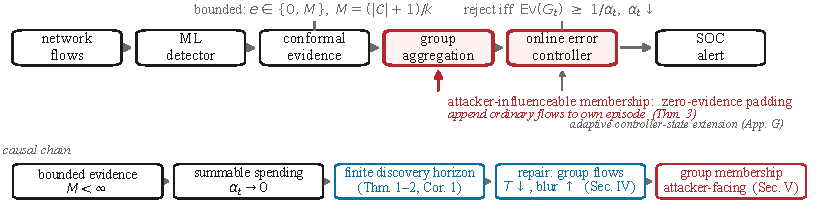
\includegraphics[width=0.72\textwidth]{fig1_chain.pdf}
\caption{The statistical trust layer and the causal chain this paper follows. Evidence entering the
controller is bounded by $\ceil=(\nCal+1)/k$; against a level that decays along a rejection-free run
this yields a finite discovery horizon for two arrival-time controller families (\cref{sec:feasibility}).
Grouping repairs feasibility by reducing $T$ (\cref{sec:granularity}) and, when the grouping key is one
the attacker can co-occupy, makes the composition of each tested hypothesis attacker-facing, which
zero-evidence padding exploits (\cref{sec:attack}). Padding leaves the malicious flows and their detector scores unchanged and only appends ordinary flows
to the same tested hypothesis; exact minimum sizing is oracle, and the state-free implementation instead
over-provisions using only the attacker's own episode size.}
\label{fig:system}
\end{figure*}

%% =======================================================================================
\section{Statistical Trust Layer and Evaluation Model}\label{sec:model}

\subsection{Bounded evidence and online decisions}\label{sec:controllers}

Flows $x_1,x_2,\ldots$ arrive in timestamp order and a detector $f$ produces scores $s_i=f(x_i)$. A
benign calibration set $\Cal$, disjoint from training and preceding deployment, converts each score into
threshold conformal evidence. Let $K_i=1+\#\{c\in\Cal:s_c\ge s_i\}$ be the rank of $s_i$ from the top of
the calibration scores (ties count against the test flow). For a rank depth $1\le k\le\nCal+1$, the
flow e-value is
\begin{equation}\label{eq:evalue}
e_i=\frac{\nCal+1}{k}\,\mathbf 1\{K_i\le k\},
\end{equation}
with $\mathbb E[e_i]\le1$ under the null and the relevant exchangeability premise, and $p_i=\min(1,1/e_i)$.
The construction is
deliberately two-point: a flow either reaches the calibration tail or receives zero. Its central
operational property is the hard ceiling
\begin{equation}\label{eq:ceiling}
\ceil=\frac{\nCal+1}{k}.
\end{equation}
No detector score generates evidence above $\ceil$: this is the finite resolution of deterministic
rank-based conformal evidence~\cite{vovk2005alrw,hennhofer2026resolution}, not a feature of our
detector; randomised smoothing removes the floor, and \cref{app:taxonomy} prices what that buys.

We write $\alpha$ for the target error level a procedure is run at and $\alphat$ for the possibly far
smaller level it \emph{offers} at step $t$; the two are distinct throughout, so $\alpha_T$ always means
the level offered at step $T$ and never $\alpha$ times $T$. At hypothesis $t$ a procedure offers
$\alphat$ and rejects when
\begin{equation}\label{eq:reject}
\Ev(G_t)\ \ge\ 1/\alphat .
\end{equation}
Equations~\eqref{eq:ceiling} and~\eqref{eq:reject} are the spine of the paper: \emph{no detector score
can create evidence above $\ceil$, so a rejection is possible at step $t$ only when
$\alphat\ge1/\ceil$.} We use e-LOND as the guarantee-bearing baseline, since it controls $\FDR$ under
arbitrary dependence given marginally valid group e-values~\cite{xu2024elond}, and instantiate the
finite-horizon results on LOND, e-LOND, e-LORD and LORD++; further online procedures and escape
mechanisms are evaluated in \cref{app:feasibility}. Throughout, $q=\alpha=0.05$, $w_0=0.025$ and $k=1$.
We evaluate two deployment regimes, which differ only in the spending sequence; we write
$(\gamma_j)_{j\ge1}$ for a spending sequence and $\gamma_t$ for its value at step $t$. The
\emph{horizon-free} regime, $\gamma_j=j^{-1.6}/\zeta(1.6)$, written $\gamma_j\propto j^{-1.6}$ below,
models uninterrupted operation when the terminal horizon is not known in advance. The \emph{horizon-aware} regime uses the horizon-uniform
allocation $\gamma_j=T^{-1}\mathbf 1\{j\le T\}$, written $\gamma_j=1/T$ for short, which knows the
stream length in advance and maximises the smallest cold-start level over $1,\ldots,T$; it is the strongest cold-start benchmark \cref{cor:budget} covers. Comparing the
two separates a structural property of the merger from a configurable property of the controller.

\subsection{Grouped security hypotheses}\label{sec:grouping}

A SOC rarely investigates one flow at a time, so we group flows into episodes $G_j$ using pre-committed
metadata and a time bucket; the headline unit is a source--destination host pair in a two-hour bucket.
The controller receives the arithmetic mean
\begin{equation}\label{eq:mean}
\Ev(G_j)=\frac1{m_j}\sum_{i\in G_j}e_i,\qquad m_j=\lvert G_j\rvert .
\end{equation}
The mean is a valid e-merging rule at every fixed arity under arbitrary dependence and, unlike a
maximum, does not grow systematically with group size, so it is the symmetric rule we evaluate.

\emph{Guarantee scope.} Reading an empirical e-LOND run as $\FDR$-controlled requires marginally valid
\emph{group} e-values under the pre-committed grouping and ordering rule, a modelling premise stated
as \cref{assump:groupval} and audited in \cref{app:validity}; \cref{tab:deps} records which results
rest on it.

\subsection{Threat model}\label{sec:threat}

The defender correctly implements detector, calibration, grouping, aggregation and controller; no attack
relies on an implementation flaw. The adversary controls traffic from an attacker-operated or
compromised host, and can open ordinary connections to the destination it is already attacking within
the same time bucket. Because the episode key is $(\mathrm{SrcIP},\mathrm{DstIP},\text{bucket})$, those
connections enter the same tested hypothesis. The adversary does not modify the detector, the
calibration code, the stored scores or its own malicious flows; it seeks to suppress the alert on its
own grouped activity. Whether ordinary traffic really contributes zero evidence is measured rather
than assumed: \cref{sec:replay} realises it on LSPR23 with a pool of real flows selected before
deployment from network-observable frequency alone, and \cref{sec:transferattack} repeats the attack
on AIT with genuine benign traffic sent to the attacked victims.

Two attack-knowledge levels are kept distinct throughout.
The \textbf{exact attack cost} $r^{\star}_t$ uses the realised group evidence and the live controller
level, so it is an oracle lower bound on what an attacker must spend. \textbf{State-free
over-provisioning} uses only the attacker's own episode size and a fixed multiplier
(\cref{sec:paddingcost}).

Groups closing in the same bucket need an order. Our main results use the \textbf{canonical} order, a
deterministic hash of the group's own metadata key with collisions broken on the key. It reads no
arrival time, so appending flows to one group moves no other hypothesis, which is what keeps the
group-validity premise intact on the attacked stream; it is a canonicalisation, not a security mechanism
(\cref{sec:transfer}). The initial first-flow arrival order is an attacker timing lever and the most
detector-favourable order we audit; it is retained in the appendix as a labelled optimistic upper bound
on LSPR23 detections, and contrasts that run under it say so.

\subsection{Data and chronological protocol}\label{sec:data}

LSPR23~\cite{lspr23} contains 16,353,511 flows from the Locked Shields live-fire exercise over 161.5
hours, of which 1,644,599 (10.06\%; $0.48$--$0.81\%$ of episodes) are malicious. We sort by timestamp
and use chronological training, benign calibration and deployment blocks (calibration and test 15\% of
$N$ each), with no random mixing across time. The five deployment positions are correlated
chronological views of one exercise, not five datasets and not independent replications: adjacent
blocks overlap, and the training pools are nested. We therefore report the windows separately, never
pool them, and read 0.62 as a robustness check rather than confirmatory replication; the exact split
geometry is \cref{app:splits}. Two detector seeds change the scores but no feasibility quantity; seeds are never pooled.

The detector is HistGradientBoosting over the protocol and 32 flow timing and volume features, a
standard choice so that changes in alert behaviour are attributable to the trust layer rather than to a
novel classifier; a second, host-conditioned detector adds six strictly causal host-context features
(\cref{sec:transferattack}). AIT-LDSv2.0~\cite{aitlds} supplies an external
benign-inclusive transfer test in which attacked hosts also receive real ordinary traffic. Features,
preprocessing and implementation checks are in \cref{app:procedures}.

Positions 0.55 (primary) and 0.62 (secondary) were fixed before any validity diagnostic existed. At
$k=1$ only $0$--$3$ benign deployment flows reach the calibration tail at each of the four non-stress
windows, so the diagnostic is far too weak to establish validity. At position 0.85,
46 benign flows fire, $50.9\times$ the nominal rate, refuting marginal e-validity
($\mathbb E[e]\approx51$): 0.85 is a \emph{known-invalid} stress window. We use it only for algebraic
results and for mechanism or cost measurements that need no valid evidence, and label it at every use.

Unless a sentence, caption or table says otherwise, every measured number is detector seed 0 under the
canonical within-bucket order at the stated window, in the horizon-free regime; \cref{app:conventions}
states the reporting conventions in full.

%% =======================================================================================
\section{Bounded Evidence Creates a Finite Discovery Horizon}\label{sec:feasibility}

Detection power asks whether malicious activity produces strong evidence. \emph{Feasibility} asks
whether even the strongest admissible evidence could be accepted by the controller. The rejection
rule~\eqref{eq:reject} and the ceiling~\eqref{eq:ceiling} give a necessary condition for a rejection at
step $t$,
\begin{equation}\label{eq:feas}
\alphat\ \ge\ 1/\ceil ,
\end{equation}
which is fixed by $\nCal$, $k$ and $T$ before a detector is evaluated. A step is \textbf{evidence-feasible} when \eqref{eq:feas} holds. The
\textbf{discovery horizon} $t^{\star}$ is the last evidence-feasible step of a rejection-free run;
beyond it the run is \textbf{absorbed}, and its operational consequence is \textbf{structural silence}
--- the controller would reject nothing even if every later hypothesis carried the maximum admissible
evidence. A procedure is \textbf{cold-start feasible through $T$} when a rejection remains possible at
every $t\le T$ before its first rejection. Recall can be lost to a weak detector, a rare attack or an
unlucky order; structural silence is settled by $\nCal$, $k$ and $T$ alone.
The results of this section are feasibility statements about the rejection rule: they need neither
\cref{assump:groupval} nor valid e-values, which enter only when a run is read as carrying its nominal
$\FDR$ guarantee (\cref{tab:deps}).

\subsection{One headline result, two controller forms}\label{sec:horizon}

\begin{theorem}[Finite discovery horizon, multiplicative family]\label{thm:family1}
Let the evidence be bounded by $\ceil<\infty$ and the controller run without restart, with
$\alphat=\alpha\,\gamma_t\,g(\mathcal H_{t-1})$, $\gamma\ge0$, $\sum_t\gamma_t\le1$ and
$g\le c_g(R_{t-1}+1)^d$ for the rejection count $R$ and some $d\ge0$ (which the step below uses; every
procedure we cover has $d\in\{0,1\}$). Since $R_{t-1}\le t-1$, a rejection is possible at
$t$ only if $\gamma_t t^d\ge1/(\alpha c_g\ceil)$. If $\gamma_t t^d\to0$, only finitely many steps are
feasible on a rejection-free run; if that set is non-empty it has a last element $t^{\star}$ and the run
is absorbed from $t^{\star}+1$ onward, and if it is empty the run is absorbed from step $1$. No monotonicity of $\gamma$ is needed: a set of steps that is
finite already has a maximum.
\end{theorem}

\begin{theorem}[Finite discovery horizon, lag-sum family]\label{thm:family2}
Let the evidence be bounded by $\ceil<\infty$ and
$\alphat=w_0\gamma_t+\sum_j a_j\gamma_{t-\tau_j}$ over prior rejection times $\tau_j<t$, with
$w_0\ge0$, $0\le a_j\le\alpha$, $\gamma\ge0$ and $\sum_t\gamma_t<\infty$. During a rejection-free run of length $\Delta$ every lag
is distinct and at least $\Delta$, so $\alphat\le(w_0+\alpha)\sum_{u\ge\Delta}\gamma_u$. The tail sum
tends to zero, so $\Delta^{\star}=\min\{\Delta:(w_0+\alpha)\sum_{u\ge\Delta}\gamma_u<1/\ceil\}$ is finite
and the run is absorbed once $\Delta\ge\Delta^{\star}$, with no monotonicity assumption on $\gamma$.
\end{theorem}

The two statements are the same argument in the two shapes an arrival-time level takes: under either
form the level offered along a long rejection-free run falls below the fixed floor $1/\ceil$, and after
the last feasible step no future evidence can restore an alert without changing the mechanism. \Cref{thm:family1} covers LOND, e-LOND and e-LORD;
\cref{thm:family2} covers LORD++, and $\gamma_j\propto j^{-1.6}$ satisfies both conditions; \cref{app:proofs} gives the proofs and the exact scope of each hypothesis.

\emph{Contribution relative to prior observations.} Huo et al.~\cite{huo2024realtime} state the
conformal floor $1/(\nCal+1)$ and report the poor online-testing behaviour it produces for LOND,
SAFFRON and ADDIS (all defined in \cref{app:procedures}). \Cref{thm:family1,thm:family2} identify the general mechanism that turns that
behaviour into structural infeasibility: for two arrival-time controller forms, the set of
evidence-feasible steps is finite and every sufficiently long rejection-free run becomes permanently
unable to report a discovery. It names the \emph{procedure-and-sequence pairs} it binds, makes the
infeasible state \emph{absorbing} rather than a gradual loss of power, and covers e-value as well as
p-value procedures; \cref{cor:budget} then gives the rate at which calibration must grow to avoid it. Together, \cref{thm:family1,thm:family2} and \cref{cor:budget}
turn prior qualitative observations about finite conformal resolution and small online levels into an
ex-ante systems criterion: before deployment, $(\nCal,k,T)$ determines whether any admissible
observation can be reported, and \cref{sec:granularity} identifies grouping as the design variable
that moves this boundary.

\subsection{The best-case calibration--horizon exchange rate}\label{sec:exchange}

Before its first rejection a procedure offers only its cold-start budget. Write $c_0$ for the
\emph{cold-start coefficient} multiplying the spending weight: $c_0=w_0$ for a level-$w_0$ procedure
such as LORD++ and $c_0=\alpha=2w_0$ for LOND/e-LOND. Among non-negative sequences with total mass at
most one, the horizon-aware uniform allocation $\gamma_t=T^{-1}\mathbf 1\{t\le T\}$ maximises $\min_{t\le T}\gamma_t$, and
therefore the cold-start horizon (proof in \cref{app:proofs}).

\begin{corollary}[Horizon-uniform feasibility]\label{cor:budget}
Cold-start feasibility over a horizon $T$ --- every step $t\le T$ evidence-feasible before the first
rejection, which the ceiling decides and detection power does not --- requires $\nCal\ge k/\alpha_T-1$,
for $\alpha_T$ the level offered at step $T$. Under the horizon-uniform allocation
$\gamma_t=T^{-1}\mathbf 1\{t\le T\}$, where $\alpha_T$ is also the smallest level offered over the
horizon, the condition is necessary \emph{and} sufficient and reads
\[
\nCal\ \ge\ \frac{kT}{c_0}-1 .
\]
The requirement is a scale-free count ratio $k/c_0$: at $k=1$ it is $20$ calibration units per
hypothesis for LOND/e-LOND and $40$ for LORD++, whatever the unit is --- exactly $20T-1$ and $40T-1$
over a horizon $T$, the ratio being the rate rather than the count.
\end{corollary}

\Cref{cor:budget} gives the best achievable cold-start scaling over every pre-committed allocation, and
turns the evidence ceiling into a deployment sizing rule: the count ratio $k/c_0$ is independent of the
dataset and of the alerting unit, so the required calibration size falls in direct proportion to the
number of tested hypotheses, which \cref{sec:granularity} exploits; its calendar form is not, because
calibration and deployment produce units at different rates (\cref{app:feasibility}). Kr\"onert et
al.~\cite{kronert2024fdr} derive an algebraically related equality for a \emph{windowed} procedure;
\cref{sec:related} states how the two objects differ. We report feasibility as the allocation-optimal
(horizon-uniform) cold-start ratio
\begin{equation}\label{eq:rho}
\rho_p=\frac{\ceil\,c_{0,p}}{T}=\frac{(\nCal+1)\,c_{0,p}}{kT}.
\end{equation}
Under the horizon-uniform allocation, $\rho_p\ge1$ is exactly cold-start feasibility through $T$ for
procedure $p$, necessary and sufficient by \cref{cor:budget}; for another pre-committed allocation
$\gamma$ the minimum-level ratio is $\rho_p(\gamma)=\ceil\,c_{0,p}\min_{t\le T}\gamma_t\le\rho_p$.
Throughout, $\rho$ denotes this horizon-uniform ratio, with the threshold at $1$ for whichever controller
is plotted.

The consequence at security scale is immediate (\cref{fig:envelope}). For an uninterrupted horizon equal to all 16,353,511 flows in the trace, with every flow
tested, \cref{cor:budget} asks for about $3.3\times10^{8}$ calibration flows for LOND/e-LOND and
$6.5\times10^{8}$ for LORD++. The first of
those is $20$ times the entire exercise: the requirement would not be met by devoting \emph{every}
one of its 16,353,511 flows to calibration, let alone the $1.8$--$2.4$ million a benign block that
precedes a deployment window actually supplies. The shortfall is the count ratio $k/c_0$ itself, so scaling
calibration and deployment in the same proportion leaves it unchanged. That is the \emph{cheapest} sequence: under the horizon-free $\gamma\propto j^{-1.6}$ the same
horizon needs about $1.6\times10^{13}$ for LOND/e-LOND and $3.2\times10^{13}$ for LORD++.

\begin{figure}[t]
\centering
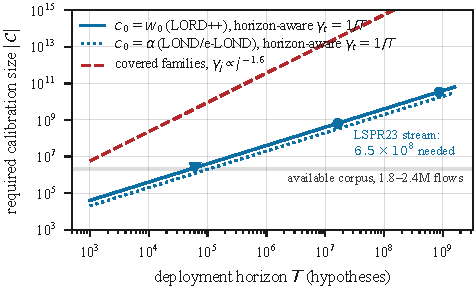
\includegraphics[width=0.70\columnwidth]{fig2_envelope.pdf}
\caption{Calibration size needed to keep a rejection possible over a horizon $T$ ($k=1$, $w_0=0.025$).
The horizon-aware uniform allocation is the cheapest cold-start allocation, and under it the requirement
is linear in $T$ for every procedure covered by \cref{thm:family1,thm:family2}, differing only through
$c_0$; the plotted horizon-free $\gamma\propto j^{-1.6}$ curve grows as $T^{1.6}$, so linearity is the
best case rather than the general rule. Procedures outside those families, for which the
absorbing-horizon predicate is not defined, are compared in \cref{app:feasibility}. The grey band is the
$1.8$--$2.4$M calibration flows these windows supply.}
\label{fig:envelope}
\end{figure}

\subsection{Feasibility is not detection power}\label{sec:feasnotdet}

The bound is necessary, not sufficient, and the two properties come apart in the direction that matters. Grouping into two-hour host-pair episodes reduces $T$ to 31,568--57,368 and makes the
horizon-uniform requirement feasible for e-LOND in all five windows ($\rho=2.13$--$3.34$), yet
the horizon-free sequence still concentrates useful level in a short prefix: before any discovery only
the first 748--902 hypotheses can reject at all, $1.6$--$2.6\%$ of the stream. Whether a near-ceiling
malicious episode lands inside that prefix then becomes decisive, and under the canonical order the
primary window yields three e-LOND detections out of 275 malicious episodes and the secondary window
eleven (\cref{tab:costcurve}).

Those counts are a property of the spending sequence, not of the evidence ceiling. The flow-granularity shortfall above is allocation-optimal already: it is what
\cref{cor:budget} requires under the \emph{best} sequence, so no reallocation removes it. The grouped
counts are not. At the two-hour unit the horizon-aware uniform allocation is feasible ($\rho=2.13$) and
detects $105$ of 275 malicious episodes at the primary window with no false discoveries, against three
under $\gamma\propto j^{-1.6}$ (\cref{tab:costcurve}). Two further configurations agree, neither of
them exotic (\cref{app:feasnotpower}). The two regimes answer different questions --- horizon-free spending exposes the
anytime deployment's short evidence-feasible prefix; horizon-aware spending, or a restart, restores
substantial detection power --- and \cref{sec:costcurve} prices the attack under both.

Under the canonical order the five positions detect $3$, $11$, $0$, $0$ and $34$ episodes; two of the five
are zero, not from absorption but because no episode's evidence clears its own step there, and the 34
belong to the stress window, whose evidence is not a valid e-value.

The cleanest contrast is a better detector that alerts less: adding six strictly causal host-context
features raises AUROC from 0.916 to 0.954 at the primary window but reduces e-LOND detections from 18 to
two (first-flow, both legs), while $\nCal$, $k$ and $T$ --- and hence $\rho$ in \eqref{eq:rho} --- are
unchanged, so ranking quality moves power but cannot move the feasibility boundary.
\Cref{app:feasibility} reports the full matrices, an Isolation Forest contrast
and a low-prevalence analysis in which the probability that e-LOND \emph{ever} rejects falls to
$0$--$40\%$ while $\rho$ does not move.

\subsection{Procedures outside the theorems}\label{sec:escapes}

The finite-horizon result applies to arrival-time controllers whose effective spending index advances
with elapsed hypotheses or rejection lags. Selective index advancement, as in ADDIS, can avoid that
elapsed-time decay, while history-wide procedures such as online e-BH fall outside the arrival-time
predicate altogether because they reconsider earlier hypotheses: \eqref{eq:feas} is not defined for a
decision that is not taken against a level fixed at arrival. These mechanisms change the source of the
constraint rather than making evidence scale irrelevant, and neither is free ---
\cref{app:state} shows that an index conditioned on observed evidence is itself attacker-controllable
(taxonomy and measurements: \cref{app:feasibility}).

%% =======================================================================================
\section{Grouping Restores Feasibility by Changing the Security Unit}\label{sec:granularity}

\Cref{cor:budget} turns the alerting unit into a design variable: if the calibration corpus cannot grow,
the direct way to restore feasibility is to reduce $T$ by testing groups of flows rather than individual
flows. Replacing flow-level hypotheses by grouped episodes lowers the horizon from $T_{\mathrm{flow}}$
to $T_{\mathrm{group}}$ and changes the allocation-optimal requirement --- the \emph{minimum}
calibration size over pre-committed spending allocations --- to
\begin{equation}\label{eq:exchange}
\nCal_{\min}+1=\frac{kT_{\mathrm{group}}}{c_0},
\end{equation}
so the required value of $\nCal+1$ falls in direct proportion to the number of tested hypotheses.
Grouping is therefore not a heuristic that happens to improve power: for the covered procedures under
uninterrupted control it buys cold-start feasibility at that exchange rate. Coarsening an
attacker-co-occupiable key is not by itself a defence: it changes feasibility and attack cost but
retains the membership surface. Coarsening from the host pair to the source host raises the primary
window's canonical detections from $3$ to $46$ under the horizon-free sequence, and raises the median
suppression cost with them, from $24$ to $496$ added flows --- both figures are oracle lower bounds,
as every $r^{\star}_t$ here is. Coarsening the key therefore changes
feasibility, alert semantics and the cost of exploitation at once. A key the attacker cannot cheaply
co-occupy would instead be a genuine membership defence, but the operational keys we evaluate are
built from endpoints for which the attacker controls one side. We evaluate five grouping
families a SOC would recognise over six bucket widths plus a whole-deployment bucket, 35 configurations
in all at each window and seed (\cref{app:granularity}; \cref{apptab:grouping} tabulates the primary
window at seed 0, and feasibility depends on $T$ alone); every family shows the predicted linear relation between hypothesis count and required calibration, and
each becomes feasible once the bucket is coarse enough. Source-host
grouping is feasible at every bucket, collapsing each window to $763$--$24{,}043$ episodes, so the
barrier can be bought off with an ordinary SOC unit.

The price is semantic resolution, and it has to be measured against a denominator that does not move.
Episode recall is not comparable across bucket widths, because the definition and number of positives
change with the unit, so we fix an atomic evaluation reference: each malicious
source--destination episode in a five-minute bucket is one atom, whatever alerting bucket the controller
uses. For each issued alert, \textbf{alert blur} is the number of distinct atomic malicious units that
alert represents. We measure blur under first-flow ordering, which produces alerts at every bucket
width, so granularity varies while the ordering rule does not. At the
primary window a five-minute alert has blur $1.0$; the mean blur rises to
$7.2$ at one hour, $16.1$ at the two-hour headline unit and $38.5$ at one day
(\cref{fig:granularity}). Fixed atomic coverage rises at the same time, but the alert no longer localises which fine-grained
activity is responsible.

The operation that restores feasibility also decides which flows share one hypothesis; because
endpoints, services and timing are partly attacker-influenceable, the defender buys a rejectable
hypothesis by making its composition attacker-facing.

\begin{figure}[t]
\centering
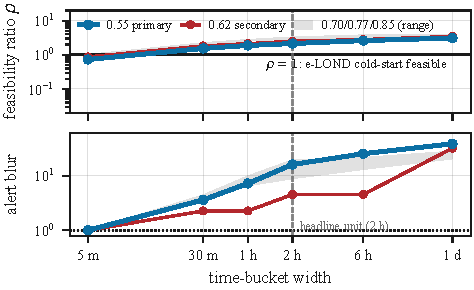
\includegraphics[width=\columnwidth]{fig3_granularity_body.pdf}
\caption{Coarsening the source--destination bucket buys feasibility (top: the feasibility ratio
$\rho$ of \eqref{eq:rho} rises through $1$) and spends resolution (bottom: alert blur, the number of
fixed five-minute atomic malicious units per issued alert). Primary and secondary windows are drawn as
series and the remaining three as a shaded range; seed 0. The two-hour headline unit is marked.}
\label{fig:granularity}
\end{figure}

%% =======================================================================================
\section{Attacker-Influenceable Group Membership Enables Padding Evasion}\label{sec:attack}

\subsection{The attack, in plain language}


An attack episode is a source--destination pair within a two-hour bucket; the attacker can open
additional ordinary connections to the same destination before the bucket closes, and those join the
same tested hypothesis. They do not alter the malicious flows or their detector scores, but under
the two-point construction an ordinary flow that does not reach the calibration tail contributes exactly
zero, so appending $r$ of them changes the controller's input from $F_m(e_1,\ldots,e_m)$ to
$F_{m+r}(e_1,\ldots,e_m,0^{r})$ and lowers the aggregate evidence. The next result rules out any
alert-capable symmetric aggregation rule that would ignore the padding while retaining validity.
Suppressing a specified alert is likewise a security statement about that rule and the realised
levels, needing neither \cref{assump:groupval} nor valid e-values (\cref{tab:deps}).

\subsection{Symmetric alerting and arbitrary padding invariance are incompatible}\label{sec:impossibility}


\begin{definition}[$\theta$-padding-robustness, attainment]\label{def:padding}
A family $\{F_N\}_{N\ge1}$ of e-merging functions is $\theta$-padding-robust, for $\theta>1$, if for every
$m\ge1$, every finite $x\in[0,\infty)^m$ with $F_m(x)\ge\theta$ and every integer $r\ge0$,
$F_{m+r}(x,0^{r})\ge\theta$. It
\emph{attains} $\theta$ if some finite input has $F_m(x)\ge\theta$.
\end{definition}

Attainment excludes rules that can never fire, such as $F\equiv1$ (\cref{app:attain}).

\begin{theorem}[Symmetric padding impossibility]\label{thm:padding}
No family of symmetric e-merging functions that attains $\theta$ is $\theta$-padding-robust, for any
$\theta>1$. Quantitatively, for every symmetric e-merging family, every $m\ge1$, every finite
$x\in[0,\infty)^m$, every $\theta>1$ and every integer $r\ge0$,
\[
F_{m+r}(x,0^{r})<\theta\qquad\text{whenever}\qquad r>\frac{\sum_i x_i}{\theta}-m .
\]
\end{theorem}

\begin{proof}[Proof idea]
Vovk and Wang~\cite[Prop.~3.1]{vovk2021evalues} show that the arithmetic mean \emph{essentially}
dominates every symmetric e-merging function: $F(e)>1$ implies $\mathrm{mean}(e)\ge F(e)$. A case split therefore gives
$F_N(x)\le\max\{1,\mathrm{mean}(x)\}$ on finite inputs. Padding gives
$\mathrm{mean}(x,0^{r})=\sum_ix_i/(m+r)$, which falls below $\theta$ once $r>\sum_ix_i/\theta-m$, and
attainment supplies an $x$ to which this applies. The mean meets the bound with equality, so the
quantitative statement is tight. \Cref{app:proofs} gives the full proof, the scaled-rule edge case, and
an independent negatively-dependent special case.
\end{proof}

\emph{Contribution of \cref{thm:padding}.} The mathematical ingredient is known; the security property
and its cross-arity consequence are not. Vovk and Wang's domination
result~\cite[Prop.~3.1]{vovk2021evalues} is that ingredient, which we use rather than reprove, and it is
stated at a fixed arity $K$: e-merging theory asks which rule is best for combining a \emph{given} set of
e-values. Our adversary changes the set, by adding members to its own hypothesis.
\Cref{def:padding} introduces the cross-arity robustness property that deployment needs, and the
theorem establishes an exact incompatibility within the symmetric e-merging class: a family can be
invariant to arbitrary zero-evidence additions or capable of crossing an alert threshold, but not both,
so a symmetric rule is vulnerable at precisely the alert thresholds it can attain (\cref{app:attain}). Its
attainment hypothesis is met whenever a symmetric merger issues an alert at the relevant threshold. The
mean attains the quantitative bound, which yields the exact attack cost \eqref{eq:rstar}, plotted per
alert in \cref{fig:attacks}; consequently,
replacing the arithmetic mean with another symmetric merger cannot repair the vulnerability.

\begin{figure*}[!t]
\centering
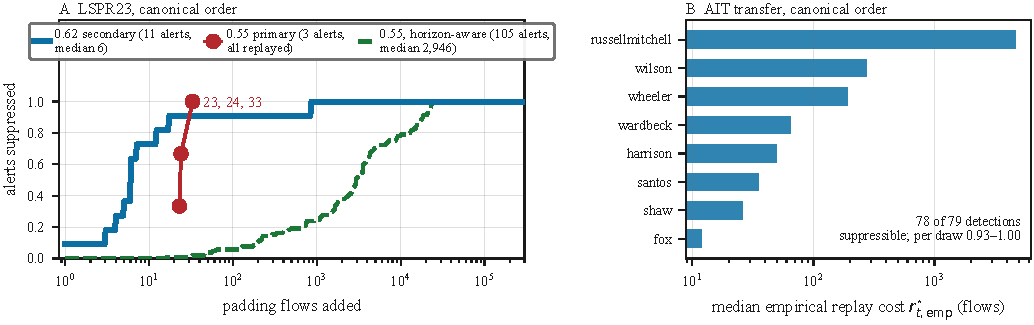
\includegraphics[width=0.72\textwidth]{fig4_padding_body.pdf}
\caption{Cost of suppressing one alert, canonical order, seed 0. \textbf{A}: LSPR23. The three
primary-window alerts (points, $23$/$24$/$33$ flows) are the horizon-free alerts that per-alert
real-flow replay suppresses, and the solid curve is the secondary window's eleven; the dashed curve is the same primary
window under the max-min-optimal horizon-aware allocation, which alerts far more often and is
correspondingly dearer to silence (\cref{tab:costcurve}). \textbf{B}: the AIT transfer, per-organisation median empirical replay cost $r^{\star}_{t,\mathrm{emp}}$,
at or above the zero-pad lower bound $r^{\star}_t$ (equal for seven of eight organisations); replay
success is evaluated separately. Pad construction is black-box. The stress window and the first-flow
arms are \cref{fig:padsens}.}
\label{fig:attacks}
\end{figure*}

\subsection{Exact cost, and what the attacker must know}\label{sec:paddingcost}


For the mean let $S_t=\sum_{i\in G_t}e_i$ and $m_t=\lvert G_t\rvert$ for the group tested at step
$t$; the padded evidence is $S_t/(m_t+r)$. If the unpadded group is rejected at level $\alphat$, the
exact attack cost --- the minimum number of zero-evidence additions that makes it fail --- is
\begin{equation}\label{eq:rstar}
r^{\star}_t=\lfloor S_t\alphat\rfloor-m_t+1 ,
\end{equation}
written $r^{\star}$ when the step is clear. Constructing such a pad is black-box --- ordinary traffic on
a common service to the host already under attack, in the same bucket --- but \eqref{eq:rstar} reads
$S_t$, the live level $\alphat$ and the unperturbed trajectory: it is the per-alert exact attack cost
of \cref{sec:threat}.

We use two attacker-knowledge models and report three cost summaries. Under oracle knowledge,
$r^{\star}_t$ is the minimum cost of suppressing one alert on the unperturbed trajectory,
$\sum_{t\in\mathcal D} r^{\star}_t$, over the set $\mathcal D$ of baseline true detections, is the
counterfactual per-alert sum of those individually priced pads, and
$J_{\mathrm{seq}}$ is the total cost of a greedy sequential oracle on the attacked trajectory. Under
\statefree\ knowledge, the attacker instead uses a fixed multiplier $c$ and needs only its own episode
size. \Cref{tab:costcurve} reports the three summaries.

What the attacker must know is settled by a separate measurement, not read off the exact attack cost.
A \statefree\ attacker can over-provision using only its own episode size. Multiplying its own episode
by $c$, appending $(c-1)m_t$ flows, defeats an alert whenever $c\ge1+r^{\star}_t/m_t$. A fixed multiplier
requires no access to $S_t$, $\alphat$ or $\nCal$ at attack time: on LSPR23, $c=10$ --- the smallest of
the multipliers we evaluate, $c\in\{2,3,5,10,100\}$, that does so --- suppresses every canonical
horizon-free alert (seed 0) at the primary and stress windows, the two arms with stored per-episode arities, at higher but measured
cost; at the secondary window one canonical alert ($m_t=22$, $r^{\star}_t=859$) needs $c=41$. Against the
horizon-aware controller the joint rerun of \cref{sec:costcurve} gives a sharper statement, and it is
exact.

\begin{corollary}[Horizon-uniform feasibility ratio as a dilution threshold]\label{cor:dilution}
Run e-LOND under the horizon-uniform allocation, so that $\alphat=(\alpha/T)(R_{t-1}+1)$ with
$R_0=0$, on arithmetic-mean group evidence whose flow e-values are bounded by $\ceil$, and write
$\rho=\rho_{\text{e-LOND}}=\ceil\alpha/T$, the horizon-uniform ratio \eqref{eq:rho} for e-LOND. Suppose no hypothesis other than the attacker's own
episodes carries evidence at or above the cold-start threshold $T/\alpha$, and the attacker
multiplies every one of its own episodes by an integer $c\ge1$, appending $(c-1)m_t$ zero-evidence
flows to an episode of arity $m_t$. If $c>\rho$, the attacked trajectory is rejection-free. If
$c\le\rho$ and some attacker episode attains $\ceil$, it is not rejection-free. Hence the smallest integer
multiplier that suffices for every stream satisfying the hypotheses is
$c_{\mathrm{int}}=\lfloor\rho\rfloor+1$.
\end{corollary}

For one given stream the smaller integer $\lfloor c_{\mathrm{crit}}\rfloor+1$ suffices, with
$c_{\mathrm{crit}}\le\rho$ the largest attacker evidence times $\alpha/T$ and equality whenever an attacker
episode attains the ceiling, as one does at each evaluated window (proof in \cref{app:proofs}). Under the corollary's assumptions, the ratio that decides cold-start feasibility in \cref{sec:feasnotdet}
is also the universally sufficient dilution threshold for all attacker-owned cold-start alerts, and
\cref{app:ait} measures it where they fail. Here $\rho$ is $2.13$ and $2.49$, so $c=3$ suffices and $c=2$ does not: against the
horizon-aware controller, multiplying \emph{every} own episode by $c=3$ silences it at both windows,
and the corollary's hypothesis on the other hypotheses holds there, since the one horizon-aware false
discovery at the secondary window fires only at a level raised by earlier detections and disappears
with them. What every multiplier needs is the attacker's own arity $m_t$, which on LSPR23 is free --- all 674 detected episodes sit on host pairs
carrying no benign traffic, so the attacker counts its own flows, needing no estimate of $S_t$, $\alphat$
or $\nCal$. \Cref{app:nonoracle} gives the over-provisioning factors, the variants we test, and the one
first-flow arm where no multiplier suffices.

\subsection{A stronger controller raises the per-alert attack price, not padding robustness}\label{sec:costcurve}

\begin{table*}[t]
\centering
\caption{Detection and padding costs under horizon-free and horizon-aware allocation, with detector,
grouping and canonical order fixed, at seed 0. $r^{\star}_t$ is the per-alert oracle cost,
$\sum_{t\in\mathcal D} r^{\star}_t$ the per-alert sum over the true detections in the row (the set
$\mathcal D$), and $J_{\mathrm{seq}}$ the greedy oracle
sequential attacker's cost on the re-run attacked trajectory (\cref{sec:costcurve,apptab:joint}).
``true det.'' counts rejected malicious episodes; ``FDP'' is realised, not guaranteed.}
\label{tab:costcurve}
\footnotesize
\setlength{\tabcolsep}{8pt}
\begin{tabular}{@{}llrrrrr@{}}
\toprule
Window & allocation & true det. & FDP & median $r^{\star}_t$ & $\sum_{t\in\mathcal D} r^{\star}_t$ & $J_{\mathrm{seq}}$ \\
\midrule
0.55 primary & horizon-free & 3 & 0.000 & $24$ & $80$ & $30$ \\
\quad & horizon-aware & 105 & 0.000 & $2{,}946$ & $627{,}495$ & $5{,}650$ \\
\midrule
0.62 secondary & horizon-free & 11 & 0.000 & $6$ & $926$ & $859$ \\
\quad & horizon-aware & 107 & 0.009 & $3{,}908$ & $977{,}567$ & $9{,}992$ \\
\bottomrule
\end{tabular}
\end{table*}

\Cref{eq:rstar} is increasing in $\alphat$, so \emph{the cost of suppression is set by the level the
alert fired at}, and a controller that alerts more readily is proportionally dearer to silence, alert
by alert; we measure both ends of the range our configurations span (\cref{tab:costcurve}). Under
the horizon-free $\gamma\propto j^{-1.6}$ the primary window issues three canonical alerts, each firing
just under the evidence ceiling, and each falls to a median of $24$ added flows. Under the
horizon-aware uniform allocation --- the allocation \cref{cor:budget} proves max-min optimal, feasible
at both windows, $\rho=2.13$ and $2.49$ --- the same window, detector, episodes and order issue $105$
alerts at zero observed false discoveries, and the median per-alert cost rises to $2{,}946$ flows;
summing the per-alert costs of the true detections along the unperturbed trajectory gives
$\sum_{t\in\mathcal D} r^{\star}_t=627{,}495$ to clear the whole set, an upper bound on the cost of jointly suppressing
that set rather than a joint minimum, since removing an early alert lowers the rejection count and so
lowers the level, and with it the cost, of every alert after it; the secondary horizon-aware arm's
one false discovery is not in that sum. Within the unbounded-membership model of \cref{thm:padding},
spending allocation cannot eliminate padding; it only changes the finite cost $r^{\star}_t$, which
every alert in both arms has. Admission control changes that model, and can
block pads whose required membership exceeds the cap.

How much lower the joint cost is, we measure with a joint controller-state rerun: the zero-evidence
pads that the real-flow replay of \cref{sec:replay} validates are propagated through the e-LOND
trajectory, which is re-run over the padded stream (\cref{apptab:joint}: canonical order, seed 0, both
windows). Applying every per-alert pad at once and re-running the controller under the canonical order leaves no true detection standing in
either regime at either window, and the one horizon-aware false discovery disappears with them. A
sequential attacker that pads each of its own episodes against the level the attacked trajectory
actually offers pays far less, because e-LOND's level carries the factor $R_{t-1}+1$: with no earlier
alert left standing, every later alert is priced at the cold-start level. At the primary window under
the canonical order this attacker pays $5{,}650$ flows in total ($J_{\mathrm{seq}}$) against the per-alert sum of
$627{,}495$, and $9{,}992$ against $977{,}567$ at the secondary window; over the alerts it pads, the
median pad is $48.5$ and $33$ flows rather than the horizon-aware $2{,}946$ and $3{,}908$, and $13$ and
$4$ alerts need no pad at all, because they fired only at a level that earlier detections had raised.
The horizon-aware price is therefore a price per alert, earned by the controller's own detections.
Suppressing early detections keeps subsequent testing levels at or near their cold-start values;
consequently, the sequential pads remain small and their joint total $J_{\mathrm{seq}}$ is far below
the per-alert sum $\sum_{t\in\mathcal D} r^{\star}_t$, though still one to two orders of magnitude above the
horizon-free totals of $30$ and $859$; and $J_{\mathrm{seq}}$ is the cost of one greedy oracle strategy
on this stream and therefore an upper bound on the minimum joint cost.

That distinction decides what the pad looks like: against the per-alert attacker a padded
primary-window episode has median arity 63 against the horizon-free controller, and 5\% of deployment
episodes are at least that large --- unremarkable; against the horizon-aware controller the median
padded arity is $2{,}989$, which only $0.22\%$ of episodes reach. The sequential attacker's pads are
small again: median padded arity $91$ at the primary window and $55$ at the secondary, reached by
$3.8\%$ and $4.3\%$ of episodes. So a per-host-pair cap on flows per bucket, the obvious control outside the trust layer, must be
priced against the attacker that adapts to it: we re-run the sequential attacker under each cap,
letting an alert fire whenever hiding it would exceed the cap. At
a cap of $100$ under the canonical order, $96$ of the $105$ horizon-aware primary-window alerts still
fire: $44$ because their pad would not fit even at the cold-start level, and $52$ because those first
alerts raise $R$ and price every later pad above the cap; at the secondary window $79$ of $107$ fire
($33$ and $46$). At $300$ the protection is far weaker than the per-alert reading suggests, $19$ and
$60$ alerts firing where $m_t+r^{\star}_t>n$ predicts $91$ and $95$, and at $1{,}000$ the sequential
attacker silences both windows. The cap costs $3.4\%$ and $2.9\%$ of benign episodes truncated at
$100$, an arity-disruption rate; we do not model what truncation does to their scores. The cap leaves
the attacker a residual set it can still silence, and against the horizon-free arm the same caps cost
the attacker \emph{nothing}: all three alerts stay suppressible at any cap of $100$ or more, and reaching them needs a cap of $30$ that
truncates $7.4\%$ of benign traffic. The pad is cheap and non-exceptional in the horizon-free regime; in
the horizon-aware regime it is large only for an attacker that lets other alerts stand, and a tight cap
protects there because the first alert it forces into the open prices the rest above it, on the two
windows and the sampled caps we evaluate.


\subsection{Does the closed form predict the implemented pipeline?}\label{sec:replay}

Priced against the running level $1/\alphat$ at each detected episode's step (\cref{tab:main}), the
canonical primary window yields three e-LOND detections whose costs are 23, 24 and 33 added flows, and
the eleven canonical secondary-window detections have a median cost of six (\cref{fig:attacks}). Those
costs are arithmetic on stored evidence. To test them against the implemented detector we construct a
weak-attacker pool using network-observable frequency alone: the most common protocol--port pair in
the training prefix, which precedes both calibration and deployment, so no attack labels, detector
outputs, calibration scores or deployment traffic enter the choice. None of 20,000 sampled pool flows
reaches the conformal tail at the primary window (one-sided 95\% upper bound $1.5\times10^{-4}$ on the
firing probability). Injecting these real flows into each detected episode suppresses it at exactly
the closed-form threshold~\eqref{eq:rstar}: all $3/3$ canonical primary-window detections, at the
predicted $23$--$33$-flow thresholds, and all $11/11$ at the secondary window, where the measured cost
equals the closed form on every episode and the median is six flows.

The horizon-aware regime replays the same way. Against the horizon-aware controller --- $105$ true
detections at the primary window with no observed false discovery, and $107$ at the secondary
alongside one false discovery, realised FDP $0.009$ --- per-alert real-flow replay suppresses
$105/105$ and $107/107$ true detections at their original controller levels, on every draw. Because
the per-alert pad is two orders of magnitude larger than at the cheap arm, a single pool flow reaching the
conformal tail would add the whole ceiling to $S_t$; across all $845{,}691$ flows the pool contains at
the primary window, \emph{none} reaches the tail, so replaying from it reproduces the closed form
exactly rather than approximately, and the full-pool zero count tightens the bound above to
$3.5\times10^{-6}$, which is what \cref{app:pools} prices the residual risk at. Across the two windows, replay therefore covers fourteen horizon-free alerts, at recall
$0.01$ and $0.03$, and $212$ horizon-aware true detections, at recall $0.38$ and $0.27$.

Replay evaluates each alert separately at the controller level it received on the unperturbed run; it
is not a joint rerun of the altered controller trajectory. The e-values are measured --- real flows,
the shipped detector --- but the aggregation and the controller level are then arithmetic on the
unperturbed trajectory, so what is demonstrated here is that real ordinary traffic carries no
evidence; the joint controller-state rerun of \cref{sec:costcurve} then propagates zero-evidence
pads, which is what such traffic is, through the re-run e-LOND trajectory. On LSPR23 the pool is
service-level,
drawn from the modal training-prefix protocol and port across the window rather than from traffic to
the victim, because every attacked host pair here is $100\%$ malicious and supplies no such traffic;
that is precisely the gap the AIT transfer closes, where the pads are real benign-to-victim flows.
Which pool the flows are drawn from barely matters (\cref{app:pools}); the \emph{selection rule} does,
since the modal service over the deployment window can be the attacker's own flood, which scores highly
and does not dilute.

Ordering changes which alerts are issued, not the conditional result: every alert produced by any of the fifty audited pre-committed orders has a finite exact cost
\eqref{eq:rstar}, so the order changes \emph{which} episodes are there to attack rather than whether
they can be (\cref{app:padwindows}).

\subsection{Is the result an artefact of a flow-only detector or of attack-only host pairs?}\label{sec:transferattack}

\begin{table}[t]
\centering
\caption{Core padding evidence in the horizon-free regime at detector seed 0, under the canonical
order except where the order column says otherwise. ``det.'' counts true e-LOND detections; ``cost'' is, on LSPR23, the exact zero-pad per-alert cost
$r^{\star}_t$ \eqref{eq:rstar} against the running level, an oracle lower bound, and on AIT, marked
(emp.), the empirical replay median $r^{\star}_{t,\mathrm{emp}}$, at or above the closed form by
construction (\cref{apptab:aitsupp} lists both); ``suppr.'' counts detections suppressed by per-alert real-flow replay (per-draw success $0.93$--$1.00$
on AIT). The joint row is the campaign total (\cref{apptab:joint76}). Full arms: \cref{app:attacks}.}
\label{tab:main}
\footnotesize
\setlength{\tabcolsep}{3pt}
\begin{tabular}{@{}llrlr@{}}
\toprule
Setting & order & det. & cost & suppr. \\
\midrule
LSPR23 0.55 primary & canonical & 3 & 23, 24, 33 & 3/3 \\
LSPR23 0.62 secondary & canonical & 11 & med.\ 6 & 11/11 \\
AIT flow-only, 8 orgs & canonical & 79 & med.\ 12--4{,}650 (emp.) & 78/79 \\
AIT flow-only, joint & canonical & 79 & $244{,}250$ total & 78/79 \\
AIT host-cond., 8 orgs & first-flow & 63 & med.\ 43--8{,}471.5 (emp.) & 57/63 \\
\bottomrule
\end{tabular}
\end{table}

\begin{table*}[t]
\centering
\caption{One representative of each way out of \cref{thm:padding}. LSPR23 two-hour host-pair episodes;
the aggregation-cap and weighting sweeps run under first-flow order, the per-host-pair volume cap
under the canonical order. The measurements behind each row are in \cref{sec:costcurve,app:defences}.}
\label{tab:defenses}
\footnotesize
\setlength{\tabcolsep}{6pt}
\begin{tabular}{@{}>{\raggedright\arraybackslash}p{4.0cm}>{\raggedright\arraybackslash}p{5.4cm}>{\raggedright\arraybackslash}p{7.2cm}@{}}
\toprule
Design response & Gain & Cost / boundary \\
\midrule
Capped normalisation $\sum_ie_i/n_0$ & Invariant to members appended below the cap $n_0$ &
Leaves the symmetric e-merging class above $n_0$; validity-preserving caps detect nothing
(\cref{apptab:caps}) \\[2pt]
Pre-committed asymmetric weights~\cite{wang2025admissible} & Valid invariance to \emph{appended} flows &
A few \emph{leading} flows defeat every scheme that keeps the mean's recall; a larger reach costs about
$58\%$ of it (\cref{tab:asym}) \\[2pt]
Group-calibrated maximum & Padding-robust aggregate & The smaller calibration unit destroys
feasibility: no alerts at the primary or secondary window (\cref{sec:groupcal}) \\[2pt]
Per-host-pair volume cap \emph{(outside the merging class)} & Blocks pads above the cap; an early
forced alert can raise later pad costs & Truncates benign episodes; leaves residual suppression;
ineffective in the horizon-free arm (\cref{sec:costcurve}) \\
\bottomrule
\end{tabular}
\end{table*}

A detector could defend by conditioning each flow on host history, making repetitive padding anomalous; we test that boundary in two stages. First, on LSPR23 we add six strictly causal host-context features:
prior connection counts, distinct-peer counts and failed-connection fractions. With the host
context recomputed causally as each pad arrives, the pads still contribute zero evidence and both
host-conditioned targets remain suppressible at the primary window (seed 0, horizon-free, first-flow)
and at the stress window (\cref{apptab:r7host}). LSPR23 cannot settle the
benign-inclusive question, however: every host pair carrying attack traffic is 100\% malicious, so it
has no real ordinary-to-victim pool.

Second, AIT-LDSv2.0 provides eight organisations in which attacked hosts also serve real benign traffic.
For each held-out organisation we train on the other seven, calibrate on in-organisation benign flows
preceding the first attack, run the same two-hour host-pair/e-LOND pipeline, and suppress each detected
episode by replaying real benign-to-victim traffic (200 draws). Across the flow-only folds, 78 of 79
true detections are suppressible under the canonical order, at per-draw success $0.93$--$1.00$ and a
per-organisation median cost of $12$--$4{,}650$ flows, above the zero-pad closed form $r^{\star}_t$
wherever a pad fires; the eight runs issue $83$ rejections, so four are false discoveries, a pooled
realised $\FDP$ of $0.048$. Recomputing the host context throughout accumulation, the same chain at all
eight organisations issues $63$ host-conditioned true detections and suppresses $57$ of them under
first-flow order (\cref{tab:main}). The six exceptions are episodes no draw cleared within twice the
zero-pad cost --- a bound on the replay budget, not a demonstration that they cannot be padded. The
channel is the accumulated context: a pad scored in it can itself fire, adding the ceiling instead of
diluting.
First-flow resequencing gives 84 of 85, at higher cost (\cref{app:attacks}).
Both counts price each alert at the level it received on the unperturbed run. Re-running the controller
over the padded stream prices the campaign: at $40\%$ and $15\%$ of the per-alert sums it leaves one and
none of the $79$ and $80$ canonical-order detections standing, and $24$ and $27$ when the attacker may
draw only on traffic the victim already had (\cref{apptab:joint76}).


%% =======================================================================================
\section{Design Alternatives and System Implications}\label{sec:fixes}

\subsection{Theorem~\ref{thm:padding} localises where a defence must act}

\Cref{thm:padding} localises the mitigation boundary: padding robustness cannot be obtained by
substituting another alert-capable symmetric merger, so it must come from membership or admission
control, a different calibrated unit, or an asymmetric rule. We measure one representative of each
route (\cref{tab:defenses}); each shifts the tradeoff rather than removing it. The per-host-pair
volume cap marks the boundary most sharply: it acts outside the symmetric merger, does
not protect the low-level horizon-free regime, and under the horizon-aware allocation a tight cap can
force an early alert to remain visible, raising later e-LOND levels so that subsequent pads exceed the
same cap (\cref{sec:costcurve}), at a measurable benign-truncation cost.


\subsection{Three implications for deployment}

\textbf{Size the evidence against the horizon before tuning the detector.} The first calculation is
\cref{cor:budget}, not an AUROC comparison. If calibration cannot support the intended horizon, detector
tuning cannot repair the shortfall; nor can switching among the procedure--sequence pairs covered by
\cref{thm:family1,thm:family2} while their stated decay conditions remain in force.

\textbf{Choose the grouping rule as part of the security specification.} Grouping fixes both the horizon
and what an alert means, so a deployment report should state the calibration-to-hypothesis ratio and a
fixed-denominator resolution measure such as alert blur; restart trades a deployment-wide guarantee for
a per-epoch one (\cref{app:feasibility}).

\textbf{Threat-model the trust layer, not only the classifier.} Any field that determines group
membership can become attacker-facing, and so can any state a future testing level is conditioned on
(\cref{app:state}); a metadata-keyed order keeps a pad from shifting unrelated hypotheses, a public
hash can be ground, and a keyed hash only reprices insertion (\cref{sec:transfer}), none of which touches
padding.

%% =======================================================================================
\section{Scope and Limitations}\label{sec:discussion}

\subsection{What each claim depends on}\label{sec:dependency}

\Cref{tab:deps} separates the algebraic, empirical and nominal-guarantee claims. Any claim that the
nominal $\FDR$ guarantee applies to these empirical runs is conditional on the group-validity premise
(\cref{assump:groupval}, group-local validity), which \cref{app:validity} audits; the available diagnostics neither
establish nor refute it, and \cref{sec:groupcal} prices the constructive alternative.

\subsection{Limitations}\label{sec:limitations}

\emph{Empirical breadth.} One live-fire exercise supplies the main chronology (\cref{sec:data}), and
its third window, 0.85, is the known-invalid stress window, admitted for mechanism and cost only;
AIT-LDSv2.0 is a second, benign-inclusive transfer test, not broad cross-domain validation. LSPR23
lacks a reliable flow-to-campaign identifier, so the operational units are episodes, and the five-minute
atom is a stable evaluation denominator rather than externally validated incident truth.

\emph{Attack cost is a curve, not a constant.} Every per-alert cost we report is conditional on the
configuration that produced the alert, because \eqref{eq:rstar} scales with the offered level, and it
prices one alert while the controller keeps working; the joint controller-state rerun of
\cref{sec:costcurve} shows, on two windows and one seed, that suppressing early detections keeps later
levels near their cold-start values and the joint cost far below the per-alert sum. That rerun
assumes the attacker pads exactly the episodes it owns, which the labels identify and which on LSPR23
carry no benign traffic, and its pads carry zero evidence; a pool with a positive firing rate would
raise $J_{\mathrm{seq}}$; the full-pool zero count gives a one-sided $95\%$ upper bound of
$3.5\times10^{-6}$ on that rate, which the rerun does not sample. We make no claim about where in either range a given deployment sits; what is configuration-independent is
\cref{thm:padding}, that the cost is finite. On a benign-inclusive stream the attacked episode also
contains benign flows the attacker cannot see, so a \statefree\ attacker knows only a lower bound on
$m_t$ and must inflate further.

\emph{Detector and grouping scope.} The transfer covers the six causal host features and the causal
accumulation model we implement, for one already-active attacker--victim pair with pinned distinct-peer
counts; it shows neither that every host-aware detector is vulnerable nor what padding from many new
peers or a high-volume flood does. The AIT transfer is reported under the
canonical order with first-flow as a measured sensitivity, and its host-conditioned arm runs at all
eight organisations but only under first-flow (\cref{tab:main}). The LSPR23 joint rerun covers zero\nobreakdash-evidence pads; the AIT
joint arms sample real pads, and their \texttt{wilson} host costs are upper bounds.

\emph{Theorem scope.} The finite horizon applies to the procedure-and-sequence pairs of
\cref{sec:horizon} under uninterrupted operation and to the sparse-evidence closure variants; smoothing,
restart, deferred decisions, other evidence constructions and faster-growing history terms change the
mechanism or the guarantee rather than refuting the boundary. We do not claim that online FDR control is generally unusable. \Cref{app:state}\label{sec:stateptr}
extends the analysis to ADDIS's evidence-conditioned spending index, an extension rather than a main
empirical claim.


%% =======================================================================================
\section{Related Work}\label{sec:related}

\textbf{Online FDR and finite conformal resolution.} LOND, LORD, SAFFRON, ADDIS, e-LOND, online e-BH and
e-GAI establish online error guarantees under different evidence and dependence
assumptions~\cite{javanmard2015lond,javanmard2018lord,ramdas2017lordpp,ramdas2018saffron,tian2019addis,xu2024elond,wang2022evaluebh,fischer2025onlineebh,egai2025},
building on $\alpha$-investing~\cite{foster2008alpha}, safe testing~\cite{grunwald2024safe} and offline
FDR~\cite{benjamini1995controlling}. Alpha-death and the loss of power from small levels are
known~\cite{ramdas2017lordpp,foster2008alpha}, and the mem-e-LORD construction of~\cite{egai2025}
coincides with e-LORD before the first rejection. Huo et al.~\cite{huo2024realtime} observe the conformal floor's effect on LOND, SAFFRON and ADDIS
(\cref{sec:horizon});
Hennhofer and Preisach~\cite{hennhofer2026resolution} study resolution collapse and smoothing in a
low-data batch setting. What this literature leaves open is the composed question a deployment has to
answer first: given $\nCal$, $k$ and $T$, can \emph{any} admissible observation be rejected at the
intended horizon? \Cref{thm:family1,thm:family2} answer it for two families, \cref{cor:budget} shows the
horizon-uniform boundary is attained rather than merely bounded, and the resulting escape criterion
classifies the recent closure and donation constructions~\cite{xu2026eclosure,xu2025closure} before they
are measured. Kr\"onert et al.~\cite{kronert2024fdr} derive an algebraically related equality, $n=\nu m/\alpha-1$,
and read it in the opposite direction: they tune the calibration size upward so that a \emph{windowed}
procedure's realised level is exact. \Cref{cor:budget} concerns a different object and consequence: the
infeasibility boundary of an \emph{uninterrupted} controller, below which no rejection is possible at
all; their windowing is, in our terms, the restart escape
(\cref{app:feasibility}).

\textbf{Trustworthy intrusion detection and temporal evaluation.} TESSERACT's temporal evaluation
constraints~\cite{pendlebury2019tesseract} and conformal drift systems such as
Transcend(ent)~\cite{jordaney2017transcend,barbero2022transcendent} motivate our chronological protocol.
Prior work applies online FDR control to anomaly streams~\cite{rebjock2021online} and, more directly,
combines conformal p-values with online FDR-controlled anomaly detection~\cite{farzaneh2025coad};
related lines study structured online FDR~\cite{wang2025multilayer}, conformal-risk-controlled
streaming alerting~\cite{caliburn2026} and conformal novelty detection with batch FDR
control~\cite{gao2026boundary}. These strands motivate individual components of our system but do not
analyse the horizon--grouping--padding chain studied here; we ask the complementary systems question: whether the
composed alert mechanism can fire at the intended horizon, what grouping does to alert semantics, and
whether the composition stays secure when traffic is adversarially generated. Label quality is a known
problem~\cite{engelen2021troubleshooting,liu2022error}, so we audit against an external record
(\cref{app:validity}).

\textbf{E-merging and adversarial testing.} E-merging theory characterises the admissible
symmetric~\cite{vovk2021evalues} and asymmetric~\cite{wang2025admissible} rules, both fixing the arity
that padding violates. Adversarial-testing work considers manipulated scores, perturbed p-values or
Byzantine reports~\cite{yasodharan2019nonzero,chen2024adversarialbh,zhang2025conformalevasion,zhang2025byzantine}.
Our adversary changes no detector score and corrupts no report: it changes which legitimate observations
belong to its own tested hypothesis, or supplies non-null observations that advance a public adaptive
state. \Cref{thm:padding} turns the first attack from an implementation example into a class-wide
impossibility. Batching also recovers power~\cite{zrnic2020batching} but needs within-batch independence or positive
dependence that co-located flows sharing
one calibration tail do not supply; decision deadlines~\cite{fisher2022deadlines,xu2026eclosure} are the
arbitrary-dependence-compatible continuum we run, and batching with a deployment-wide budget obeys
\cref{cor:budget} unchanged. Feedback-aware online testing folds revealed labels into the threshold with
finite-sample control~\cite{lu2026gaif,liu2025ocsarc}; \cref{app:baselines} prices simpler threshold
controllers under analyst delay.

%% =======================================================================================
\section{Conclusion}\label{sec:conclusion}

Statistical validity is not a substitute for system viability. Bounded evidence and arrival-time error
spending must be sized jointly: for the controller families we study, a mismatch makes future reporting
structurally impossible, at a calibration cost that is, at best, linear in the number of tested
hypotheses. Sufficient grouping restores cold-start feasibility, but where the grouping key is
attacker-co-occupiable and membership unbounded, the alert unit it creates is an adversarial control
surface on which every alert-capable symmetric e-merging family is vulnerable to sufficient
zero-evidence padding. Allocation then decides whether that system is nearly silent, cheaply
suppressible, or dear enough per alert for a tight volume cap to intervene --- and on the two windows we
re-ran, per-alert pricing did not characterise the joint cost. Evidence scale, controller design, alert
granularity and adversarial membership control have to be evaluated together, on the composed system.

%% =======================================================================================
%% The sections below sit BEFORE the references and do NOT count toward the 12-page body.
%% =======================================================================================

\section*{Open Science}\label{sec:openscience}

We will release the complete set of artifacts needed to reproduce every number and figure in this paper;
they exist and have been run in full at the time of submission: a single executable notebook that carries
the paper's derivations and measurements alongside the prose, the library of measurement scripts it
imports, the cached results of a full run, and a pinned environment. Cached-result mode executes in
about half a minute, renders every table and figure directly from the shipped result objects (the
figure-drawing code is part of the library, and the script that writes this paper's figures is a wrapper
over it) and requires no raw dataset. Full mode recomputes those objects from the original flow data; we
executed that mode end to end and verified that it reproduces the shipped results.

The obstacle is third-party data, on which the artifact depends in two places. LSPR23 is not ours to
redistribute but is publicly available under CC-BY-4.0 (Zenodo record 8042347), and the artifact ships the
exact preprocessing commands that turn the published CSV into the pipeline's inputs. The transfer test
additionally uses AIT-LDSv2.0~\cite{aitlds} (Zenodo record 5789064, CC-BY-4.0): the artifact ships the
per-organisation \texttt{tstat} netflow extraction and the exact malicious/benign label mapping
(\cref{app:procedures}) that turn its released packet captures into the eight-organisation netflow inputs,
following the dataset's own recipe. Full-mode reproduction therefore requires downloading both records;
the derivations, procedure implementations, attack code and cached results carry no such restriction.
They will be deposited in a fully anonymised repository within three days of submission, kept accessible
for the duration of review and not edited after that deadline, and on Zenodo for the camera-ready.

\section*{LLM Usage Considerations}

Hosted LLMs were accessed through Claude Code and Codex CLI for editorial refinement, code generation,
evaluation support, and read-only code audits. LLMs were used for editorial purposes in this manuscript,
and all outputs were inspected by the authors to ensure accuracy and originality. They are not part of
the proposed method, the released pipeline's operation or the dataset labelling. Their use was motivated
by the volume of automation, evaluation and consistency-checking code the project required within its
timeframe. Code was validated
through unit tests, per-alert real-flow replay against the closed forms, closed-form cross-checks of the
derivations, and paper-to-artifact consistency gates that recompute every reported number from the
shipped result objects; every number and reference was verified by the authors. The released artifact
contains the exact code used to produce the reported results. The authors take responsibility for all
content and any remaining errors.

\emph{Necessity, model choice and footprint.} We used the general-purpose assistants already available
in our development environment; no model was trained or fine-tuned, and no LLM is required to execute or
reproduce the released pipeline. The models were chosen because the tasks were editorial, code-generation and code-audit tasks for
which a general model suffices. The clients' session logs for this project record Claude Code (client versions 2.1.241--2.1.261) with the model identifiers \texttt{claude-opus-5}, \texttt{claude-opus-4-8},
\texttt{claude-fable-5-1} and \texttt{claude-fable-5}, and Codex CLI (client versions 0.142.3 and
0.152.1) with the model identifiers \texttt{gpt-5.5}, \texttt{gpt-5.6-terra} and \texttt{gpt-5.6-sol};
neither client records the provider-side model snapshot date, so we do not report one. We limited query
volume by working in long sessions
that batch related requests, by reusing generated code and the cached result objects rather than
regenerating them, by running every consistency gate locally as a script rather than by querying a model,
and by keeping the released pipeline free of any model call: reproducing every number and figure in this
paper requires no access to an LLM, and the artifact imports no LLM client. Provider-side energy
measurements for the assistants were not available to us, so we do not estimate their emissions. The
reported experiments themselves are CPU-only scikit-learn computations on a single workstation, a
MacBook Pro with an Apple M5 Pro system-on-chip (18 CPU cores, 48\,GB unified memory, no discrete GPU;
the pipeline uses no GPU): a full recomputation from the flow data takes about two to three hours and
the cached-result reproduction about half a minute.

\section*{Ethical Considerations}

This paper describes working attacks against a statistical trust layer for intrusion detection, so we
state our reasoning against the Menlo Report framing~\cite{menlo2012}.

\emph{Respect for persons and justice.} All measurements are made on public research datasets released
for this purpose, captured during authorised cyber-defence exercises on purpose-built ranges rather than
on production networks carrying third-party traffic. We rely on the publishers' own ethical review and
release terms and did not conduct a separate consent audit, so we make no claim about individual consent
beyond what those releases state. No attack was executed against any live network, and no personal data
is used, disclosed or re-identified.

\emph{Beneficence and responsible disclosure.} This work does not target a deployed product, and the
class of system it studies is, to our knowledge, not yet widely deployed, which is the point at which
disclosure is cheapest and most useful. It introduces no new attack on the underlying detector: it
identifies a security consequence that emerges when public statistical components are composed ---
bounded evidence, attacker-influenceable grouping and online error spending together produce an alert
layer that can become infeasible or suppressible. We report both the inexpensive and the expensive
attack regimes and evaluate representative mitigations, so that designers can assess the exposure
before deploying such a composition.

\emph{Law and public interest.} We identify a small set of host pairs whose labels we believe to be wrong
and deliberately do not publish corrected labels: rewriting a public dataset's labels from our own
detector's tail would be circular, and the pairs were identified using test-split information. We report
the direction of the error instead.

\bibliographystyle{IEEEtran}
\bibliography{refs}

\appendices
%% Both aliases are positional: labels set BEFORE this line keep their body types ("Section III-D"),
%% labels set after become "Appendix F-C".  Dropping the subsection line reintroduces "section F-C".
\crefalias{section}{appendix}
\crefalias{subsection}{appendix}
\crefalias{subsubsection}{appendix}
\crefname{appendix}{Appendix}{Appendices}\Crefname{appendix}{Appendix}{Appendices}
%% Unlimited, but reviewers are not required to read appendices, so nothing the BODY'S ARGUMENT needs
%% lives only here.  Appendix G is the exception by design: it is an extension the body cites twice and
%% never leans on.  Each appendix opens with the question it answers and its takeaway.

%% ---------------------------------------------------------------------------------------
\section{Proofs and Exact Scope}\label{app:proofs}

\emph{Question answered.} What exactly do the body's four formal results assume, and what does the
$\FDR$ reading of an empirical e-LOND run assume on top of them? \emph{Takeaway.} The feasibility
theorems need only a finite evidence ceiling and the stated level form; the padding impossibility needs
only the symmetric e-merging class; the group-validity premise below is needed by neither, and only by
the nominal guarantee.

The body states \cref{thm:family1,thm:family2,cor:budget,thm:padding}. This appendix adds the
group-validity premise, the exact scope of each body result, and five further results the body cites;
all proofs follow, verified numerically in the released artifact.

\subsection{The group-validity premise}\label{app:groupval}

Using the mean at variable, metadata-selected arity needs a group-level premise, and different
controllers need different things of it: e-LOND and online e-BH control $\FDR$ under arbitrary
dependence given only \emph{marginally} valid group e-values, whereas the p-value procedures need
conditional super-uniformity, independence or monotonicity. The guarantee-bearing claims therefore use
e-LOND.

The conditioning is stated \emph{per hypothesis}. For group $j$ let $\mathcal M_j$ be the
$\sigma$-field generated by the pre-committed metadata that determines that hypothesis and nothing else:
the grouping key, the membership indicators and arity $m_j$, the group's position in the pre-committed
within-bucket order (hence the spending weight $\gamma_j$ it is offered), and the horizon $T$. It
carries no information about any other group's composition. Pre-committed means chosen before the scores
and not score-adaptive.

\begin{assumption}[Group-local metadata-conditional validity]\label{assump:groupval}
For every benign flow $i$ of a true-null group $G_j$, $\mathbb E[e_i\mid\mathcal M_j]\le1$; for the
two-point e-value, equivalently $\Pr(K_i\le k\mid\mathcal M_j)\le k/(\nCal+1)$.
\end{assumption}

\begin{lemma}[Group-level marginal e-validity]\label{lem:groupval}
Under \cref{assump:groupval}, every true-null group with $m_j>0$ has a marginally valid group e-value,
$\mathbb E[\Ev(G_j)]\le1$, for random membership and arity and under arbitrary within- and between-group
dependence.
\end{lemma}

Conditioning on $\mathcal M_j$ fixes membership and $m_j$, so linearity gives
$\mathbb E[\Ev(G_j)\mid\mathcal M_j]\le1$ and the tower property removes the conditioning (proof
below). The premise is stronger than the unconditional validity split conformal supplies, it is a
genuine modelling assumption (endpoint and service metadata can correlate with the timing and volume
features that drive the score), and it is \emph{not} established by the dataset. \Cref{tab:scope}
separates every claim by what it needs.

\subsection{Exact scope of the finite-horizon theorems}\label{app:horizonscope}

\Cref{thm:family1} covers LOND, e-LOND and e-LORD, the last through the equivalence e-LORD $=$ e-LOND
under $\gamma_t=\omega_t\prod_{j<t}(1-\omega_j)$~\cite{egai2025}. That equivalence is a hypothesis and
not a remark, and it needs two things of the weights, not one. They must be \emph{deterministic
functions of the index}, fixed before deployment --- predictability in the filtration, which is all
online FDR normally asks, would make $\gamma$ a history-dependent random object, and
\cref{thm:family1}'s condition is a statement about a sequence. And they must satisfy
$\omega_j\in[0,1]$: pre-commitment alone gives fixedness only, and a pre-committed $\omega_1=2$ yields
$\gamma_1=2$ and $\gamma_2<0$, breaking both $\gamma\ge0$ and the budget. Under
$\omega_j\in[0,1]$ the partial sums telescope, $\sum_{t\le n}\gamma_t=1-\prod_{j\le n}(1-\omega_j)\le1$,
which gives \cref{thm:family1} the non-negativity and the budget. It does not give the decay
condition, and the sparse sequence of the next paragraph is itself induced by a deterministic
$\omega\in[0,1]$, so $\gamma_t t^d\to0$ has to be checked for the induced $\gamma$, as it is for the
$\gamma_j\propto j^{-1.6}$ pair we run.

\Cref{thm:family2} covers LORD++ ($a_1=\alpha-w_0$, $a_j=\alpha$ for $j\ge2$). What is covered is a
procedure \emph{together with} its spending sequence, not a named procedure in the abstract:
summability alone is not enough for \cref{thm:family1} at $d=1$, since
$\gamma_{2^n}=n^{-2}/\zeta(2)$ for $n\ge1$, with $\gamma_t=0$ elsewhere, sums to exactly one yet has
$2^n\gamma_{2^n}\to\infty$. That example refutes the \emph{hypothesis}, not the conclusion: the same
sequence has $\gamma_t\to0$ and so is still absorbed at $d=0$. The decay condition therefore has to be
checked per pair, and it is asymptotic: for $\gamma_j\propto j^{-1.6}$, $t\gamma_t\to0$ so $d=1$ holds,
whereas a level growing quadratically in the rejection count would escape the argument. A
horizon-uniform $\gamma$ is supported on $t\le T$, so an asymptotic decay condition is met trivially
and decides nothing; it needs none, because before any rejection the level is the constant $c_0/T$
across the horizon, feasibility there is all-or-nothing, and \cref{cor:budget} decides it exactly.

The two families are not equally strong, and the difference is worth stating. \Cref{thm:family1}'s
bound $\alphat\le\alpha c_g\gamma_t t^d$ uses only $R_{t-1}\le t-1$, so it holds whatever the history:
the feasible set is a fixed set of indices and absorption does not depend on the run being
rejection-free. \Cref{thm:family2}'s bound is driven by the length $\Delta$ of the \emph{current}
rejection-free gap, so its absorption is conditional on such a gap occurring. A lag-sum procedure that
keeps rejecting keeps its level up --- for LORD++ under $\gamma_j\propto j^{-1.6}$ with a rejection at
every step, $\alphat$ climbs from its cold-start value towards $0.039$, and every step of that run is
feasible once $\nCal\ge91$, the binding step being the cold start itself. This is why the
paper's claims are cold-start claims: the horizon is the horizon of a rejection-free prefix, which is
the state a deployment starts in and, on these streams, mostly stays in. The theorems are scoped
deliberately: they do not say every online FDR procedure dies, and \cref{app:feasibility} locates the
procedures that escape.

\subsection{Attainment and the symmetric class}\label{app:attain}

Every rejection threshold in our setting is $\theta=1/\alphat>1$, and attainment is the hypothesis the
deployment supplies whenever an alert is possible at all: if a symmetric family ever issues an alert then
some input it receives has $F\ge\theta$, so it attains $\theta$ and \cref{thm:padding} applies to it.
\emph{Not} being $\theta$-padding-robust and attaining $\theta$ are therefore the same condition, since a
family reaching $\theta$ nowhere --- $F\equiv1$, which is padding-invariant but can never fire, because
rejection needs evidence $\ge1/\alphat>1$ --- satisfies \cref{def:padding} vacuously. For the mean rule
the body evaluates the witness is explicit: the all-firing group $x=(\ceil,\ldots,\ceil)$ attains
$\theta$ at every evidence-feasible step \eqref{eq:feas}. The implication runs only that way. Attainment is strictly the weaker condition, since it quantifies over
all of $[0,\infty)^m$ --- a scaled rule such as $\tfrac12\mathrm{mean}$ is a valid symmetric e-merging
family that attains $\theta$ somewhere yet, on two-point evidence with $\theta>\ceil/2$, can never fire
--- so what attainment excludes is only the rules that reach $\theta$ nowhere, which is all the theorem
needs. Ordinary domination by the mean is false ($\kappa+(1-\kappa)\,\mathrm{mean}$, for
$\kappa\in(0,1)$, is a counterexample), which is why the proof splits cases.

\subsection{Further results used in the body}\label{app:further}

\begin{proposition}[Donation is bounded before the first rejection]\label{prop:donation}
For donation e-LOND with parameter $\delta\in(0,1)$ and a spending sequence with $\gamma\ge0$ and
$\sum_t\gamma_t\le1$ --- the normalisation the bound relies on --- on a rejection-free prefix
$\alphat\le\delta\gamma_t/(1-\delta)$. The restriction $\delta<1$ is necessary, not cosmetic: at
$\delta=1$ the donated wealth can drive the denominator to zero and hold $\alphat$ away from zero
along a rejection-free run, so neither the bound nor absorption survives (\cref{app:proofs}). Hence donation e-LOND satisfies \cref{thm:family1}'s hypotheses \emph{along a rejection-free prefix},
with $c_g=\delta/[\alpha(1-\delta)]$ --- which is $1/(1-\delta)$ exactly when $\delta=\alpha$, the setting
we run, since \cref{thm:family1} writes the level as $\alpha\gamma_t g$ --- and $d=0$, because
that bound holds uniformly in $t$ --- $g$ itself is not constant along the prefix, since the donated
wealth grows, but $d=0$ asks for a constant bound, not a constant $g$. The instantiation matters: $d=0$ asks only for
$\gamma_t\to0$, which summability supplies, whereas $d=1$ would ask for $t\gamma_t\to0$, which it does
not (take $\gamma_{2^j}=2^{-j}$ and $\gamma_t=0$ elsewhere). That is all \cref{thm:family1} needs, since its conclusion is
itself a statement about rejection-free runs --- so the horizon stays finite and the run is absorbed. It is
\emph{not} a global member of the family: past $1/\delta$ rejections no finite $c_g(R+1)^d$ bounds the
level. The bound is a
cold-start statement only --- past $1/\delta$ rejections the denominator can vanish --- and it is sharp
where it applies. On our streams the realised donation wealth stays at most $0.12$ of a budget of $1$.
\end{proposition}

\begin{proposition}[Closure is bounded by its zero-evidence subset]\label{prop:closure}
For closed e-LOND whose subset aggregator is zero on all-zero input --- $E_S=0$ whenever $E_i=0$ for
every $i\in S$, including $S=\emptyset$ --- let $Z_t=\#\{i<t:E_i=0\}$. Then
$\alphat\le\delta\gamma_{Z_t+1}(R_{t-1}+1)$. The hypothesis is not implied by e-merging validity:
$\kappa+(1-\kappa)\,\mathrm{mean}$ is symmetric and valid yet returns $\kappa>0$ on all-zero input,
and the zero-evidence subset then certifies nothing.
\end{proposition}

\begin{corollary}[When the closure is absorbing]\label{cor:closureabsorb}
Let $H=\min\{j:\gamma_j<1/(\delta\ceil)\}$ be the first index at which the spending weight dips below
the floor --- \cref{thm:family1}'s index horizon when $\gamma$ is decreasing, as ours is --- and
$P_T=\#\{i\le T:E_i>0\}$ the number of hypotheses carrying any evidence. \emph{(i)} Along a
rejection-free run, closed e-LOND is absorbed by step $H+P_T$ whenever $H+P_T\le T$: an additive offset,
holding pathwise with no assumption beyond counting. \emph{(ii)} Asymptotically, if
$\liminf_t Z_t/t>0$ then for every $\rho'<\liminf_t Z_t/t$ there is an onset $t_1$ beyond which the
closure's effective spending index is at least $\rho' t$, so absorption occurs by
$\max\{t_1,\lceil(H-1)/\rho'\rceil\}$ --- the index is rescaled by $\rho'$ and the absorption
\emph{time} therefore stretched by $1/\rho'$, not shortened. A positive $\liminf$ permits an
arbitrarily long initial transient, which is why $t_1$ cannot be dropped. On our streams $P_T\in\{0,\ldots,152\}$, at most $0.48\%$ of
$T$, so form (i) applies and the offset is at most 152 hypotheses.
\end{corollary}

\begin{theorem}[Reach]\label{thm:reach}
Fix one hypothesis, offered level $\alphat$, whose episode has flow positions $i$. For a pre-committed
weight sequence with $\sum_iw_i\le1$, the number $P$ of positions at which a lone attack flow can fire
the rule $F(e)=\sum_iw_ie_i$ is at most $\alphat\ceil$, the quantity that governs \cref{cor:budget}.
\end{theorem}

\begin{theorem}[Front-load cost]\label{thm:frontload}
At that same hypothesis, detection is impossible once $L\ge L^{\star}(w):=\min\{L:\sum_{i>L}w_i<\beta\}$,
with $\beta=1/(\alphat\ceil)$; $L^{\star}$ is finite for every summable $w$. The threshold is \emph{sufficient}
for impossibility, and exact only when every non-prepended position carries firing evidence: with fewer
firing flows detection can already be impossible at smaller $L$, so $L^{\star}$ is an upper bound on what
the attacker must prepend.
\end{theorem}

%% Full proofs. Verified numerically in the released artifact (theory stages t15, t18, t21f,
%% t32a, t34a, t35a, t36a). Notation matches the body: M = ceil = (|C|+1)/k is the evidence
%% ceiling, every per-flow e-value lies in {0, M}, and a rejection at step t needs evidence
%% >= 1/alpha_t.

\subsection{Group-level marginal e-validity (\cref{lem:groupval})}

\begin{proof}
For a tested group $G_j$, recall $\mathcal{M}_j$ is the $\sigma$-field generated by the pre-committed
metadata that determines \emph{this} hypothesis: the grouping key, the membership indicators
$\mathbf 1\{i\in G_j\}$, the arity $m_j$, the group's position in the pre-committed stream order (and
hence the spending weight $\gamma_j$ it is offered), and the horizon $T$. It carries no information
about any other group's composition or arity, and --- as the scope note below records --- none about
the realised calibration scores. Fix a true-null group $G_j$ (all constituent flows benign) with
$m_j>0$. By linearity of conditional expectation and $\mathcal{M}_j$-measurability of the membership
indicators and of $m_j$,
\begin{align*}
\mathbb{E}[\Ev(G_j)\mid\mathcal{M}_j]
 &=\mathbb{E}\big[\tfrac1{m_j}\textstyle\sum_{i\in G_j} e_i \,\big|\,\mathcal{M}_j\big]\\
 &=\tfrac1{m_j}\textstyle\sum_{i\in G_j}\mathbb{E}[e_i\mid\mathcal{M}_j]\ \le\ 1,
\end{align*}
the inequality by \cref{assump:groupval}. Taking expectations and applying the tower property gives
$\mathbb{E}[\Ev(G_j)]=\mathbb{E}\big[\mathbb{E}[\Ev(G_j)\mid\mathcal{M}_j]\big]\le1$. No independence or
exchangeability \emph{among} the $\{e_i\}$ is used, so within-group dependence is unrestricted; and
because e-LOND and online e-BH control $\FDR$ under arbitrary dependence given marginally valid
per-hypothesis e-values, arbitrary between-group dependence is permitted as well. An empty group
($m_j=0$) tests no hypothesis; assigning it the trivial $\Ev=1$ is harmless. For the two-point
conformal e-value $e_i=\ceil\,\mathbf 1\{K_i\le k\}$ the premise $\mathbb{E}[e_i\mid\mathcal{M}_j]\le1$
is exactly $\Pr(K_i\le k\mid\mathcal{M}_j)\le k/(\nCal+1)$, since $\ceil=(\nCal+1)/k$.
\end{proof}

\emph{Why the conditioning is per hypothesis.} A single global metadata $\sigma$-field $\mathcal{M}$
will not support the attack analysis of \cref{sec:attack}. $\mathbb{E}[e_i\mid\mathcal{M}]\le1$ does
\emph{not} imply $\mathbb{E}[e_i\mid\mathcal{M}']\le1$ for a richer $\mathcal{M}'$ --- take
$e=2\mathbf 1_A$ with $\Pr(A)=\tfrac12$: against the trivial $\sigma$-field the conditional
expectation is $1$, against $\sigma(A)$ it is $2$ on $A$ --- so an adversary who enriches the stream's
metadata anywhere would, on the global reading, void the premise even for groups it never touched.
With $\mathcal{M}_j$ the statement is local and survives: padding adds flows carrying the attacked
group's \emph{own} key, so it changes no other group's key, membership or arity, and adds no
hypothesis, leaving $T$ fixed. Provided the within-bucket order is a function of group metadata alone
(the deterministic hashed-key canonical order of \cref{sec:transfer}, with collisions broken on the
key itself), every true-null group's position and $\gamma_j$ are likewise fixed, so $\mathcal{M}_j$ is
literally the same $\sigma$-field before and after the attack. Under an arrival-ordered tie-break this
fails: a pad placed before the attacked group's first flow moves that group within its bucket and can
shift a true-null group's index, hence $\gamma_j$, hence $\mathcal{M}_j$. Creating a \emph{new} host
pair is likewise outside the padding claim --- it adds a hypothesis and changes $T$, which the
horizon-uniform $\gamma_j=1/T$ reads.

\emph{Scope.} The lemma certifies the \emph{e-value} controllers (e-LOND, online e-BH) only. The
p-value procedures carry their own conditions --- conditional super-uniformity for mFDR, and
independence with monotonicity for $\FDR$ --- which this argument does not supply, and which
\cref{sec:escapes} shows ADDIS violates on this stream. The premise
$\mathbb{E}[e_i\mid\mathcal{M}_j]\le1$ is marginal over the calibration draw and test score; it is
\emph{not} validity conditional on the realised calibration scores, which are deliberately excluded
from $\mathcal{M}_j$ (the Bates adjustment supplies that stronger, calibration-conditional guarantee at
a power cost and is not required here). $\mathcal{M}_j$ is also \emph{smaller} than a global
metadata $\sigma$-field, so \cref{assump:groupval} is the weaker of the two conditional premises,
while remaining stronger than unconditional $\mathbb{E}[e_i]\le1$.

\subsection{Feasibility (\cref{thm:family1,thm:family2}, \cref{cor:budget})}

\begin{proof}[\cref{thm:family1}]
With $\alphat = \alpha\gamma_t\,g(\mathcal{H}_{t-1})$, $g \le c_g(R_{t-1}+1)^d$, and
$R_{t-1}\le t-1$, we have $\alphat \le \alpha c_g\,\gamma_t t^d$. A rejection at $t$ needs
$\alphat \ge 1/\ceil$, hence $\gamma_t t^d \ge 1/(\alpha c_g\,\ceil)$. If $\gamma_t t^d \to 0$ then only
finitely many $t$ satisfy that inequality, since a sequence tending to zero exceeds a fixed positive
constant finitely often. A finite set of indices has a maximum, so there is a last feasible index
$t^\star$ (or none at all), and every $t>t^\star$ fails the necessary condition: the run is absorbed
from $t^\star+1$. No monotonicity of $\gamma$ is needed. Requiring permanence from the \emph{first}
infeasible step would be a stronger property --- false for non-monotone $\gamma$, since feasibility can
fail once and return --- and it is not what \cref{sec:feasibility} defines.
\end{proof}

\begin{proof}[\cref{thm:family2}]
Let $\alphat = w_0\gamma_t + \sum_j a_j\gamma_{t-\tau_j}$ with $w_0\ge0$ and $0\le a_j\le\alpha$ over
rejection times $\tau_j<t$. During a rejection-free run of length $\Delta$ the last rejection is at least
$\Delta$ before $t$, so every lag $t-\tau_j\ge\Delta$ and the lags are distinct. With
$\Gamma(\Delta)=\sum_{u\ge\Delta}\gamma_u$ we have $\gamma_{t-\tau_j}\le\Gamma(\Delta)$ termwise and
$\gamma_t\le\Gamma(t)\le\Gamma(\Delta)$, so, using $a_j\le\alpha$ and the distinctness of the lags,
$\alphat \le w_0\Gamma(\Delta) + \alpha\Gamma(\Delta) = (w_0+\alpha)\Gamma(\Delta)$; the first term is
where $w_0\ge0$ is used, since $\gamma_t\le\Gamma(\Delta)$ may only be multiplied through by a
non-negative $w_0$. Since $\Gamma$ is
non-increasing and $\sum\gamma<\infty$ forces $\Gamma(\Delta)\to0$, the quantity
$\Delta^\star=\min\{\Delta:(w_0+\alpha)\Gamma(\Delta)<1/\ceil\}$ is finite; $\Delta$ only grows during
a rejection-free run, so the state is absorbing. No monotonicity of $\gamma$ is used.
\end{proof}

\begin{proof}[\cref{cor:budget} and max-min optimality of $\gamma_t=1/T$]
Before any rejection, family~I has $\alphat=\alpha\gamma_t$ and family~II has $\alphat=w_0\gamma_t$;
write the cold-start coefficient $c_0\in\{w_0,\alpha\}$, so $\alpha_T=c_0\gamma_T$. Feasibility at $T$
requires $\alpha_T\ge 1/\ceil=k/(\nCal+1)$, i.e. $\nCal\ge k/\alpha_T-1=k/(c_0\gamma_T)-1$. Under
$\gamma_T=1/T$ this is $\nCal\ge kT/c_0-1$: $kT/w_0-1$ for a level-$w_0$ procedure such as LORD++,
and $kT/\alpha-1$ for LOND/e-LOND. For optimality, a cold-start rejection is possible at every
$t\le T$ iff $\min_{t\le T}\gamma_t \ge k/((\nCal+1)c_0)$; among sequences with
$\sum_{t\le T}\gamma_t\le 1$ the value $\min_{t\le T}\gamma_t$ is maximised, at $1/T$, by the
uniform allocation: $\min_{t\le T}\gamma_t\le T^{-1}\sum_{t\le T}\gamma_t\le1/T$, since a minimum is
at most an average, and $\gamma_t=1/T$ attains it. Constraining the mass over all $t$ rather than over
$t\le T$ changes nothing, since $\sum_t\gamma_t\le1$ implies $\sum_{t\le T}\gamma_t\le1$, and the
attaining sequence satisfies the global constraint too. Hence $\gamma_t=1/T$ maximises the feasible
horizon. That same criterion supplies the corollary's \emph{sufficiency}, which is otherwise easy to
miss: under $\gamma_t=1/T$ it reads $1/T\ge k/((\nCal+1)c_0)$, i.e.\ $\nCal\ge kT/c_0-1$ once more, so
this one inequality is not merely necessary at step $T$ but sufficient for feasibility at every
$t\le T$. The two directions coincide here only because a cold-start uniform level is constant over
the horizon; for a general $\gamma$ the necessary condition at $T$ is strictly weaker than
feasibility throughout, which is why the corollary states the equivalence for $\gamma_t=1/T$ alone.
\end{proof}

\subsection{The UAI 2026 procedures (\cref{prop:donation,prop:closure})}

\begin{proof}[\Cref{prop:donation}]
Donation e-LOND sets
$\alphat = \delta\gamma_t(\lvert R_{t-1}\rvert+1) / \bigl(1 - (\delta(\lvert R_{t-1}\rvert+1)\bar W_t \wedge 1)\bigr)$
with
$\bar W_t = \sum_{i\in R_{t-1}} \gamma_i\bigl((E_i - \tfrac{1}{\delta\gamma_i(\lvert R_{t-1}\rvert+1)}) \wedge 1\bigr)
+ \sum_{i\notin R_{t-1}} \gamma_i (E_i \wedge 1)$.
with both sums running over $i<t$. Every summand is $\gamma_i$ times a quantity capped at $1$, so
$\bar W_t \le \sum_{i<t} \gamma_i \le 1$ \emph{always}. On a rejection-free prefix
$R_{t-1}=\emptyset$, so for $\delta<1$ the denominator is at least $1-\delta>0$ and
$\alphat \le \delta\gamma_t/(1-\delta)$, which is \cref{thm:family1} with
$c_g = \delta/[\alpha(1-\delta)]$ and $d = 0$: \cref{thm:family1} writes the level as
$\alpha\gamma_t g(\mathcal{H}_{t-1})$, so the constant must absorb the ratio $\delta/\alpha$, and it
reduces to $1/(1-\delta)$ exactly in the $\delta=\alpha$ setting we run. $d=0$ is the right
instantiation, not merely a valid one: on a rejection-free prefix $R_{t-1}=0$, so the displayed bound
$g\le c_g$ holds uniformly in $t$ --- $g$ itself rises with $\bar W_t$ and is not constant --- and
\cref{thm:family1}'s conclusion then needs only $\gamma_t\to0$, which $\sum_t\gamma_t\le1$ gives.
Taking $d=1$ instead would demand $t\gamma_t\to0$, which summability does \emph{not} imply
($\gamma_{2^j}=2^{-j}$, zero elsewhere, sums to one with $t\gamma_t=1$ infinitely often).

\emph{Why $\delta<1$ is required.} At $\delta=1$ the denominator is $1-\bar W_t$, which the donated
wealth drives to zero, and the conclusion fails outright. Take $\delta=1$, $\gamma_t=2^{-t}$ and
$E_t=1$ for every $t$. Then $\bar W_t=\sum_{i<t}\gamma_i(E_i\wedge1)=\sum_{i<t}\gamma_i=1-2^{-(t-1)}$
and $\alphat=\gamma_t/(1-\bar W_t)=2^{-t}/2^{-(t-1)}=\tfrac12$ for \emph{every} $t$. The run is
rejection-free because rejection needs $E_t\ge1/\alphat=2$ and $E_t=1$ --- this is why the evidence is
pinned at exactly $1$ rather than merely bounded below by it --- yet the offered level never decays, so
with any $\ceil\ge2$ every step stays evidence-feasible and the run is never absorbed. The proposition
therefore quantifies over $\delta\in(0,1)$; our runs use $\delta=\alpha=0.05$, where
$1/(1-\delta)=1.05$.

The restriction to the rejection-free prefix is not cosmetic. With $R = \lvert R_{t-1}\rvert$ the
denominator is $1 - (\delta(R+1)\bar W_t \wedge 1)$, which vanishes once $\delta(R+1)\bar W_t \ge 1$;
since $\bar W_t$ can approach $1$, that is reachable at $R+1 \ge 1/\delta$. The bound is therefore a
cold-start statement, which is exactly the state \cref{cor:budget} concerns. It is also sharp: taking
$E_i \ge 1$ for every $i$ makes $\bar W_t = \sum\gamma_i \to 1$ and the bound tight.
\end{proof}

\begin{proof}[\Cref{prop:closure}]
Closed e-LOND sets
$\alphat = \min_{S\subseteq[t-1]:\,D_t(S)>0} \delta\gamma_{\lvert S\rvert+1}(\lvert R_{t-1}\rvert+1)/D_t(S)$
with $D_t(S) = 1 + \lvert S\cap R_{t-1}\rvert - \delta E_S(\lvert R_{t-1}\rvert+1)$, where $E_S$
aggregates the evidence on $S$. Because $\alphat$ is a \emph{minimum} over admissible subsets, any
single admissible $S$ furnishes an upper bound.

Take $S = \{i<t : E_i = 0\}$, of size $Z_t$. A hypothesis carrying zero evidence is never rejected, so
$S\cap R_{t-1} = \emptyset$; and $E_S = 0$ because the aggregator is zero on all-zero input,
including the empty subset that arises when $Z_t=0$. Hence
$D_t(S) = 1 > 0$, $S$ is admissible, and
$\alphat \le \delta\gamma_{Z_t+1}(\lvert R_{t-1}\rvert+1)$.

This is the decay of \cref{thm:family1} with the time index rescaled from $t$ to $Z_t+1$. The bound
itself is unconditional and pathwise; the \emph{conclusion} that the state is absorbing is not, and
\cref{cor:closureabsorb} supplies its hypothesis.
\end{proof}

\begin{proof}[\Cref{cor:closureabsorb}]
By \cref{prop:closure}, $\alphat \le \delta\gamma_{Z_t+1}(\lvert R_{t-1}\rvert+1)$ along any run. On a
rejection-free run $\lvert R_{t-1}\rvert = 0$, so $\alphat \le \delta\gamma_{Z_t+1}$. If
$\gamma_{Z_t+1}\to0$ then $\alphat\to0$, and since the evidence is bounded above by $\ceil$
(\cref{sec:feasibility}) the offered level falls below $1/\ceil$ after finitely many steps and no
rejection is possible thereafter: the state is absorbing, which is \cref{thm:family1}'s conclusion.

\emph{Form (i), exact and finite-horizon.} Along the rejection-free run $\lvert R_{t-1}\rvert=0$, so
$\alphat\le\delta\gamma_{Z_t+1}$. Our $\gamma_j\propto j^{-1.6}$ is decreasing, so no rejection is
possible once $\gamma_{Z_t+1} < 1/(\delta\ceil)$, i.e.\ once $Z_t \ge H-1$ for
$H = \min\{j : \gamma_j < 1/(\delta\ceil)\}$, which is exactly \cref{thm:family1}'s index horizon.
Write $P_T = \#\{i\le T : E_i>0\}$. Of the $t-1$ hypotheses before step $t$, at most $P_T$ carry
positive evidence, so $Z_t \ge t-1-P_T$ for every $t\le T$ --- a counting statement, with no
assumption on the stream. Hence $Z_t \ge H-1$ as soon as $t \ge H + P_T$, and
\[
  t_{\text{closed}} \ :=\ \inf\{t : Z_t \ge H-1\} \ \le\ H + P_T .
\]
The closure therefore reaches the absorbing state within an \emph{additive} $P_T$ steps of the horizon
\cref{thm:family1} gives, whenever $H+P_T\le T$. Nothing is asymptotic and no density is assumed. For a
non-monotone $\gamma$ the same conclusion follows without the decreasing step, because $\alphat$ is a
\emph{minimum} over admissible subsets: any $H-1$ zero-evidence indices furnish an admissible $S$ and
hence the same bound.

\emph{Form (ii), asymptotic.} Suppose $\liminf_t Z_t/t = \rho > 0$ and fix any $\rho' < \rho$. By the
definition of the $\liminf$ there is a $t_1$ with $Z_t \ge \rho' t$ for all $t \ge t_1$; so
$Z_t\to\infty$ and, $\gamma_j\propto j^{-1.6}$ being decreasing to $0$,
$\gamma_{Z_t+1} \le \gamma_{\lceil\rho' t\rceil}\to0$. Substituting into \cref{thm:family1}'s
discovery-horizon computation replaces the index $t$ by $\rho' t$: the effective spending index is
rescaled by $\rho'$, so absorption is reached once both $t\ge t_1$ and $\rho' t\ge H-1$, i.e.\ by
$\max\{t_1,\lceil(H-1)/\rho'\rceil\}$. The onset $t_1$ cannot be dropped: a positive $\liminf$
constrains only the eventual density and permits an arbitrarily long initial transient. The
\emph{time} to absorption is therefore stretched by $1/\rho'$, not shortened --- a sparser
zero-evidence stream buys the closure more steps, not fewer. This holds for every $\rho'<\rho$ and \emph{not}, from this argument, at $\rho$ itself:
the liminf gives eventual domination below its value, not at it.

On our streams form \emph{(i)} is the operative one and needs no density at all. The number of
hypotheses carrying \emph{any} evidence is $P_T \in \{0,\dots,152\}$ over the ten window--seed cells,
at most $\hat p = 4.82\times10^{-3}$ of $T$, attained at position $0.85$, and $P_T=0$ at $0.70$ seed
$1$; so the horizon offset is at most $152$ hypotheses and the cap is attained (ratio $1.000000$ over
every configuration measured). The argument is specific to \emph{sparse} evidence: a stream in which
most hypotheses carry positive evidence has $P_T$ close to $T$, $Z_t$ small, and this bound says
little --- which is the regime the closure was designed for, and not a security stream.
\end{proof}

\subsection{Symmetric padding impossibility (\cref{thm:padding})}

We give a full proof (Route A) and an independent lemma (Route B) that needs no domination result.
Route B's scope is narrow and worth stating exactly: it shows that a symmetric family maps any
permutation of a mean-one two-point vector to at most $1$. That yields the impossibility only for
families whose \emph{unpadded} value on that vector already reaches $\theta$ --- the arithmetic mean
among them --- and not for the class. A symmetric valid family such as
$F_N(e)=\mathrm{mean}(e)\,\mathbf 1\{\text{not all }e_i\text{ equal}\}$ attains $\theta$ elsewhere yet
returns $0$ on Route B's unpadded vector, so Route B produces no violation for it and Route A must.
The class-wide statement and the quantitative bound are Route A's alone.

\begin{proof}[Route A (essential domination)]
Vovk and Wang's Proposition~3.1~\cite{vovk2021evalues} states that the arithmetic mean $M_K$
\emph{essentially} dominates every symmetric e-merging function: $F(e)>1\Rightarrow M_K(e)\ge F(e)$.
Ordinary domination is false ($\kappa+(1-\kappa)M_K$, for any $\kappa\in(0,1)$, is a symmetric valid counterexample), so we
use it through a case split: for finite $x$, either $F_N(x)\le1$, or $F_N(x)>1$ and then
$M_K(x)\ge F_N(x)$; in both cases $F_N(x)\le\max\!\big(1,\mathrm{mean}(x)\big)$.

We need that inequality at $(x,0^r)$, a boundary point of $[0,\infty)^N$, so we prove it directly
rather than rely on the domain of the cited proposition. Let $y\in[0,\infty)^N$, $\bar y=\mathrm{mean}(y)$,
and let $\Pi$ be a uniformly random permutation of $y$; each coordinate of $\Pi$ has mean $\bar y$, and
$F_N(\Pi)\equiv F_N(y)$ by symmetry. If $\bar y\le1$ then $\Pi$ is an admissible input, $F_N(\Pi)$ is a
constant e-variable, so $F_N(y)\le1$. If $\bar y>1$, take $E=\Pi$ with probability $1/\bar y$ and
$E=0$ otherwise; every coordinate of $E$ then has mean exactly $1$, so validity gives
$F_N(y)/\bar y+(1-1/\bar y)F_N(0)\le1$, and $F_N(0)\ge0$ yields $F_N(y)\le\bar y$. Either way
$F_N(y)\le\max(1,\bar y)$ on all of $[0,\infty)^N$, zeros included, which is what the padding step uses.
This also removes any need for monotonicity or measurability assumptions on $F_N$. Padding
$x\in[0,\infty)^m$ with $r$ zeros gives $\mathrm{mean}(x,0^r)=\big(\sum_i x_i\big)/(m+r)$, so
\[
F_{m+r}(x,0^r)\ \le\ \max\!\Big(1,\ \tfrac{\sum_i x_i}{m+r}\Big)\ <\ \theta
\ \text{ once }\ r>\tfrac{\sum_i x_i}{\theta}-m .
\]
Attainment supplies an $x$ with $F_m(x)\ge\theta$ to which this applies, so no attaining symmetric
family is $\theta$-padding-robust for any $\theta>1$.
\end{proof}

\begin{proof}[Route B (a negatively-dependent special case)]
Fix $\theta>1$ and $m$. Draw a uniformly random size-$m$ subset $S\subseteq[N]$ and set
$e_i=(N/m)\mathbf{1}\{i\in S\}$. Then $\mathbb{E}[e_i]=(N/m)\Pr(i\in S)=1$, so each $e_i$ is an
e-variable, and the vector is a permutation of $\big((N/m)\mathbf{1}_m,0^{N-m}\big)$. A symmetric
$F_N$ maps every realisation to the same constant, and a constant e-variable is $\le1$. Hence
$F_N\big((N/m)\mathbf{1}_m,0^{N-m}\big)\le1<\theta$ for all $N\ge m$: appending $N-m$ zeros to the
$m$ firing positions drives any symmetric rule below $\theta$.
\end{proof}

\emph{Tightness and attainment.} The bound is tight: the mean itself has $F_{m+r}(x,0^r)=(\sum
x)/(m+r)\ge\theta$ exactly while $r\le(\sum x)/\theta-m$. Attainment (\cref{sec:attack}) is necessary,
not cosmetic: the constant rule $F\equiv1$ is symmetric, valid and padding-invariant but never
reaches any $\theta>1$, satisfying $\theta$-padding-robustness vacuously; since rejection needs
evidence $\ge1/\alphat>1$, restricting to attaining families excludes exactly the rules that
cannot fire.

\subsection{Feasibility ratio as a dilution threshold (\cref{cor:dilution})}

\begin{proof}[\cref{cor:dilution}]
Under $\gamma_t=1/T$ the level is $\alphat=(\alpha/T)(R_{t-1}+1)$, so on a rejection-free prefix
$\alphat=\alpha/T$ and \eqref{eq:reject} rejects $G_t$ exactly when $\Ev(G_t)\ge T/\alpha$; the rule
is inclusive. \emph{Sufficiency.} Let $c>\rho$ be an integer; we show by induction on $t$ that no
rejection occurs. Suppose none has occurred before $t$, so $R_{t-1}=0$ and the level is $\alpha/T$.
If $G_t$ is not an attacker episode, $\Ev(G_t)<T/\alpha$ by hypothesis. If it is, with unpadded sum
$S_t$ and arity $m_t$, each of its flow e-values is at most $\ceil$ by \eqref{eq:ceiling}, so
$S_t\le\ceil m_t$; its padded arity is the integer $cm_t$ and the padded mean is
$S_t/(cm_t)\le\ceil/c<\ceil/\rho=T/\alpha$, using $c>\rho$ and $\rho=\ceil\alpha/T$. In either case
\eqref{eq:reject} fails at $t$ and the induction closes. \emph{Necessity.} Let $c\le\rho$ be an
integer and let some attacker episode $G_u$ attain the ceiling, $S_u=\ceil m_u$. If the attacked
trajectory were rejection-free, $G_u$ would be tested at $\alpha/T$ with padded mean
$\ceil m_u/(cm_u)=\ceil/c\ge\ceil/\rho=T/\alpha$ and rejected by the inclusive rule, a
contradiction. Hence no integer $c\le\rho$ suffices for every stream satisfying the hypotheses,
whereas the integer $\lfloor\rho\rfloor+1>\rho$ does. Two remarks. The hypothesis on the other
hypotheses cannot be dropped: a benign group rejected at the cold-start level raises $R$ and with it
every later level, and the attacker's pads are then priced above $\alpha/T$. And the threshold is
uniform over streams: for one given stream with at least one attacker episode, the same two
arguments, with $\ceil$ replaced by $\max_u\Ev(G_u)$ over the attacker's episodes, show that the
smallest sufficient integer is
$\lfloor c_{\mathrm{crit}}\rfloor+1$ with $c_{\mathrm{crit}}=\max_u\Ev(G_u)\,\alpha/T\le\rho$, and
$c_{\mathrm{crit}}=\rho$ exactly when some attacker episode attains $\ceil$. A real-valued $c$ would
make $(c-1)m_t$ non-integral; the statement is therefore made for integers, which is what an attacker
can append.
\end{proof}

\subsection{Reach and front-load (\cref{thm:reach,thm:frontload})}

Let $w=(w_1,w_2,\dots)$ be precommitted with $w_i\ge0$ and $\sum_i w_i\le1$, let
$F(e)=\sum_i w_i e_i$ with each $e_i\in\{0,\ceil\}$, and write $\beta=1/(\alphat\ceil)$ for the
weight mass a detection needs: a lone flow firing at position $i$ gives $F=w_i\ceil$, which clears
$1/\alphat$ iff $w_i\ge\beta$.

\begin{proof}[\cref{thm:reach}]
The positions at which a lone attack flow fires are $\{i:w_i\ge\beta\}$. Since $\sum_i w_i\le1$,
at most $1/\beta$ indices can carry mass $\ge\beta$, so
$P=|\{i:w_i\ge\beta\}|\le 1/\beta=\alphat\ceil$, the quantity that governs \cref{cor:budget}.
\end{proof}

\begin{proof}[\cref{thm:frontload}]
Prepending $L$ zero-evidence flows moves every attack flow to a position $>L$. Every $e_i\le\ceil$, so
$F(e)\le\ceil\sum_{i>L}w_i$, and detection requires $\sum_{i>L}w_i\ge\beta$; it is impossible once
$L\ge L^\star(w)=\min\{L:\sum_{i>L}w_i<\beta\}$. Summability gives $\sum_{i>L}w_i\to0$, so the set is
non-empty and $L^\star$ is finite for every summable $w$.

\emph{Sufficient, and exact only under a full-firing episode.} The displayed bound is attained only when
every position $>L$ fires, so $L^\star$ is the exact minimum in that case and an \emph{upper} bound
otherwise. The gap is real: for $w=(0.4,0.3,0.3,0,\dots)$ and $\beta=0.5$ the tail first falls below
$\beta$ at $L=2$, yet an episode carrying a \emph{lone} firing flow is already undetectable at $L=0$,
since $\max_i w_i=0.4<\beta$ and \cref{thm:reach} gives $P=0$. We therefore quote $L^\star$ as an
attacker's upper bound throughout.
\end{proof}

Consequently a precommitted scheme cannot simultaneously be padding-invariant (weights fixed by
absolute position), have usable power (some $w_i\ge\beta$), and make ordering robustness unbounded
($L^\star=\infty$). Concentrating weight early gives $L^\star=1$ but $P=1$; spreading it over more
than $1/\beta$ positions drives every $w_i<\beta$, so $P=0$.

\subsection{ADDIS state budget (\cref{thm:addis}) and the coincidence}

\begin{proof}[\cref{thm:addis}]
ADDIS offers $\alphat=\min\{\lambda,(\tau-\lambda)[W\gamma_{S^t-C_{0+}}+\cdots]\}$. The theorem
assumes $\lambda\ge k/(\nCal+1)$, i.e.\ the cap sits at or above the conformal floor, so that the
driving term and not the cap is what the attack has to push below $1/\ceil$; if the cap were already
below the floor no target could be rejected at $D=0$ and the budget would be zero rather than the
displayed value. With $W=w_0$
before the first rejection and $W=\alpha R$ after $R$ of them, and $0$-indexed
$\gamma_j=(j+1)^{-1.6}/\zeta(1.6)$. Precursors injected at index $0$ hold the spending index at
$S^t-C_{0+}=D$, so the driving level is $(\tau-\lambda)W\gamma_D$. The collapse of ADDIS's reward sum to
the single term $W\gamma_D$ is exact in the pre-rejection state, where $W=w_0$ and there is one active
term. After $R\ge1$ rejections each reward term carries its own selected-non-candidate lag
$\ell_j\ge0$, sitting at index $D-\ell_j$; the coefficients sum to exactly
$w_0+(\alpha-w_0)+\alpha(R-1)=\alpha R$, but $\gamma$ is decreasing, so
$\sum_j a_j\gamma_{D-\ell_j}\ge\alpha R\,\gamma_D$. The drive is therefore \emph{larger} than the
collapsed expression, feasibility survives further, and the displayed value at $W=\alpha R$ is a
\emph{lower} bound on $B^\star$ --- equality only when every $\ell_j=0$. Numerically, at
$\lambda\ceil=(\tau-\lambda)\ceil=4.5\times10^{5}$, $R=1$ and a single lag of $100$, the expression
returns $313$ while the true budget is $373$. The attack is mounted in the pre-rejection state, since the precursors precede every target. A rejection is possible only
while $(\tau-\lambda)W\gamma_D\ge1/\ceil$, i.e.
$(D+1)^{-1.6}/\zeta(1.6)\ge k/\big((\tau-\lambda)W(\nCal+1)\big)$, i.e.
$D+1\le[(\tau-\lambda)W(\nCal+1)/(k\zeta(1.6))]^{1/1.6}$. The smallest $D$ violating this is
$B^\star$. Each precursor is a group carrying exactly one firing flow, so its evidence is $\ceil/m$
and its p-value $m/\ceil$; landing in $(\lambda,\tau]$ needs $m\in(\lambda\ceil,\tau\ceil]$, whose
smallest integer is $m^\star=\lfloor\lambda(\nCal+1)/k\rfloor+1$ (the interval is non-empty because
$(\tau-\lambda)\ceil\gg1$). The total is $B^\star m^\star$, scaling as
$\lambda\nCal\,[(\tau-\lambda)w_0\nCal]^{0.625}/k^{1.625}$.
\end{proof}

\emph{Coincidence.} When ADDIS's cap binds, $\alphat=\lambda$, and the minimal suppressing pad
raises the padded p-value just past $\lambda$. Because the p-value moves in steps of one conformal
floor $1/(\nCal+1)\ll\tau-\lambda$, it lands in $(\lambda,\tau]$ and advances the index:
cap-saturation \emph{implies} landing. The converse is not forced, but on this stream every
unsaturated detection has a level four orders of magnitude below $\lambda$, so none can land, and
the observed equality (all $101$ saturated detections land) is the generic case rather than a
coincidence of this window.

\subsection{Restart FDR composition}

\begin{proof}
Restart runs $n$ controllers on disjoint epochs, each controlling its own $\FDR$ at $q$. The
deployment-wide proportion $\FDP=\sum_i V_i/(\sum_i R_i\vee1)$ is a weighted average of the
per-epoch $\FDP_i$ with data-dependent weights $R_i/\sum_j R_j$, so per-epoch control does not
bound $\mathbb{E}[\FDP]$. Indeed, suppose each epoch makes \emph{one false rejection with
probability $q$ and no rejection otherwise}. Each epoch then has
$\FDR_i=\mathbb{E}[V_i/(R_i\vee1)]=q$, yet whenever any epoch rejects every pooled rejection is
false, so the deployment-wide $\FDP$ is $1$ on that event and $0$ otherwise, and with independent
epochs $\FDR=\Pr(\text{some epoch rejects})=1-(1-q)^n$. (The neighbouring construction --- each epoch
\emph{always} rejecting once, false with probability $q$ --- instead gives pooled $\FDR=q$, so
non-composition requires the all-or-nothing epoch above and does not follow from per-epoch control
alone.) In contrast, mFDR pools: if
$\mathbb{E}[V_i]\le q\,\mathbb{E}[R_i]$ for every $i$, the mediant inequality gives
$\sum_i\mathbb{E}[V_i]/\sum_i\mathbb{E}[R_i]\le q$.

This non-composition is specific to \emph{budget reset} --- every epoch spends its own $q$, total
$nq$. A \emph{preallocated} restart --- pre-committed epoch budgets $q_1,\dots,q_n$ with
$\sum_i q_i\le q$, fixed before deployment --- instead \emph{preserves} the deployment-wide guarantee.
Since $\sum_j R_j\ge R_i$, the pooled proportion is dominated termwise,
\[
\FDP=\frac{\sum_i V_i}{\sum_j R_j\vee1}\le\sum_i\frac{V_i}{R_i\vee1}=\sum_i\FDP_i
\]
(both sides $0$ when no epoch rejects), so by linearity of expectation
$\FDR\le\sum_i\FDR_i\le\sum_i q_i\le q$ --- no independence across epochs is required (independence
enters only the $1-(1-q)^n$ counterexample above). Each e-LOND epoch delivers $\FDR_i\le q_i$ under the
same group e-validity premise (\cref{assump:groupval}); the shared calibration set only induces
between-epoch dependence, which this bound tolerates, provided the epoch boundaries and the $q_i$ are
not data-dependent. Restart therefore does not simply void the deployment-wide guarantee: it forces a
\emph{choice} --- budget reset recovers more power but controls only a per-epoch $\FDR$, whereas
preallocation keeps deployment-wide $\FDR\le q$ at a power cost (\cref{apptab:restart}).
\end{proof}


%% ---------------------------------------------------------------------------------------
\section{Procedures, Data, and Reproducibility}\label{app:procedures}\label{app:data}

\subsection{Terms}

\begin{table}[t]
\centering
\caption{Terms held distinct throughout the paper. Definitions only, so \textbf{order-invariant}: the
table reports no measurement, and the quantities defined here that are measured on a sequenced stream are
reported elsewhere. Validity is an assumption; feasibility, power and resolution are separate
consequences.}
\label{tab:terms}
\footnotesize
\setlength{\tabcolsep}{4pt}
\begin{tabular}{@{}>{\raggedright\arraybackslash}p{2.45cm}>{\raggedright\arraybackslash}p{5.85cm}@{}}
\toprule
Term & Meaning \\
\midrule
Statistical validity & the assumptions the stated $\FDR$/e-value guarantee needs (\cref{assump:groupval,lem:groupval}) \\
Feasibility & whether \emph{any} admissible evidence can cross the controller threshold \\
Detection power & whether malicious episodes actually generate sufficient evidence \\
Episode recall & recall under the \emph{current} grouping definition (moving denominator) \\
Atomic coverage & coverage of a \emph{fixed} fine-grained attack-unit denominator \\
Alert blur & number of fixed atomic \emph{reference} units one issued alert represents \\
\midrule
Per-alert padding cost $r^{\star}_t$ & zero-evidence flows that suppress one alert at the level it received on the unperturbed run, \eqref{eq:rstar}; an oracle lower bound (Surface~A). On AIT, where a pad flow can fire, the empirical replay cost $r^{\star}_{t,\mathrm{emp}}\ge r^{\star}_t$ is reported and labelled \\
Per-alert sum $\sum_{t\in\mathcal D} r^{\star}_t$ & the per-alert costs of the baseline true detections $\mathcal D$ added up on the unperturbed trajectory; an upper bound on the joint cost \\
Joint padding cost $J_{\mathrm{seq}}$ & total cost of the greedy sequential oracle when e-LOND is re-run over the padded stream, so that $R_{t-1}$ responds to the pads (the \emph{joint controller-state rerun}, Surface~A) \\
State-free multiplier $c$ & the attacker multiplies its own episode size by $c$ and reads no controller state (\cref{cor:dilution}) \\
Controller-state attack cost $B^{\star}$ & precursor hypotheses that advance ADDIS's evidence-conditioned spending index (Surface~B, \cref{app:state}); a different mechanism from the e-LOND rerun above: padding changes e-LOND's rejection state indirectly by preventing discoveries, whereas the ADDIS attack directly advances its evidence-conditioned spending index \\
\bottomrule
\end{tabular}
\end{table}

\FloatBarrier
\subsection{Procedure definitions}

Each procedure offers a level $\alphat$ and rejects $H_t$ when the evidence exceeds $1/\alphat$
(p-value procedures reject when $p_t\le\alphat$). We write $R_{t-1}$ for the rejection count, $\tau_j$
for the $j$-th rejection time, and, for the candidate-based procedures, $C_{j+}(t)$ for the number of
candidates after $\tau_j$. Transcriptions were unit-tested against literal $O(T^2)$ implementations of
the published formulas and against four identities the sources state (offline e-BH as the $t=K$ case of
online e-BH; $R(\text{e-LOND})\subseteq R(\text{online e-BH})$; e-LORD $=$ e-LOND under
$\gamma_t=\omega_t\prod_{j<t}(1-\omega_j)$; e-SAFFRON$(\lambda{=}0)=$e-LORD).
{\small\begin{align*}
\text{LOND, e-LOND:}\ &\alphat=\alpha\,\gamma_t\,(R_{t-1}+1),\\
\text{LORD++:}\ &\alphat=\gamma_t w_0+(\alpha-w_0)\gamma_{t-\tau_1}+\alpha\!\sum_{j\ge2}\gamma_{t-\tau_j},\\
\text{SAFFRON:}\ &\alphat=\min\big\{\lambda,\,(1-\lambda)[w_0\gamma_{t-C_{0+}}+\cdots]\big\},\\
\text{ADDIS:}\ &\alphat=\min\big\{\lambda,\,(\tau-\lambda)[w_0\gamma_{S^t-C_{0+}}+\cdots]\big\},\\
\text{online e-BH:}\ &\text{reject } H_i \text{ iff } E_i\ge 1/(k^\star_t\alpha\gamma_i),\\
\text{e-LORD (e-GAI):}\ &\alphat=\omega_t\big(\alpha-\textstyle\sum_{j<t}\tfrac{a_j}{R_{j-1}+1}\big)(R_{t-1}+1).
\end{align*}}%
SAFFRON (serial estimate of the alpha fraction that is futilely rationed on true null hypotheses) and
ADDIS (adaptive discarding) are the adaptive descendants of LORD, and online e-BH is the e-value
Benjamini--Hochberg procedure run at each step. SAFFRON's candidates are the $p\le\lambda$; ADDIS additionally \emph{selects} the $p\le\tau$ and counts
selected non-candidates. Here $k^\star_t=\max\{k\le t:\sum_{j\le t}\mathbf{1}\{E_j\ge
1/(k\alpha\gamma_j)\}\ge k\}$ is the online-e-BH step-up fixed point, and $\omega_t$ is the e-GAI weight
update~\cite{egai2025}, which we run \textbf{pre-committed} --- the specialisation under which the
e-LORD reparametrisation of \cref{sec:feasibility} yields a fixed summable $\gamma$, and the only one
our feasibility coverage claims. Throughout $\alpha=q=0.05$, $w_0=0.025$, $k=1$; ADDIS uses
$\lambda=0.25,\tau=0.5$, SAFFRON $\lambda=0.5$, e-SAFFRON $\lambda=0.1$, and e-GAI $\phi=\psi=0.5$,
$\omega_1=1/T$. The two spending sequences are $\gamma_j\propto j^{-1.6}$ (normalised by
$\zeta(1.6)=2.2858$, no horizon needed) and horizon-uniform $\gamma_j=1/T$ (max-min optimal, \oracle).
We do not extend the feasibility bound to e-SAFFRON at $\lambda=0.1$, a testing level the equivalence
does not cover. mem-e-LORD is a different case and the tables mark it covered: its level has the family-I
form, so \cref{thm:family1} bounds its \emph{feasibility} exactly as for e-LORD; what does not transfer
is the error-rate reading, since it controls mem-$\FDR$ rather than $\FDR$, and we never quote its
rejections as $\FDR$-controlled. The r-LOND variants inherit the classification
verbatim, their rejection sets coinciding with e-LOND's on calibrated $p$-values. For e-TOAD we use the
interpretation of the active set and step-up limit consistent with its stated limiting cases
($d_t=t\Rightarrow$ e-LOND, $d_t=\infty\Rightarrow$ online e-BH); the alternate literal reading is a
sensitivity analysis in \cref{apptab:uai26}. One equation of the compound-e construction admits two
readings (a literal snapshot and a running union of the rejection history); we report both and default
to the literal one.

\Cref{tab:procedures} gives the full procedure matrix at the primary and stress windows, including the
first-flow rejection counts the body's taxonomy (\cref{tab:taxonomy}) summarises.

\begin{table*}[t]
\centering
\caption{Procedures, assumptions, and coverage by \cref{thm:family1,thm:family2}. Power is reported at
the \textbf{primary analysis window} (0.55, $\nCal = 2{,}448{,}993$, $T = 57{,}368$ episodes, 275
malicious) and the \textbf{stress-test window} (0.85, $\nCal = 1{,}813{,}113$, $T = 31{,}568$, 255
malicious), two-hour grouping. Horizon-uniform $\gamma$ requires the stream length in advance and is
marked \oracle\ wherever it appears. The $\FDP$ column is the 0.85 stress-window value, measured against
labels where the evidence is not a valid e-value (\cref{sec:tail}); at 0.55 every $\FDP$ here is
$\le 0.010$. Which procedures are covered is position-independent; the rejection counts differ because the
two windows carry different traffic. $^\dagger$SAFFRON sits outside the letter of
\cref{thm:family1,thm:family2} because its index counts tested hypotheses, but it does not escape in
practice: it is silent for 99.3\% of the stream at 0.55 and 75\% at 0.85. Only ADDIS and online e-BH avoid the horizon's practical
consequence, and they do so differently: ADDIS's index stops advancing, a genuine escape from
arrival-time absorption, whereas online e-BH is decided by a fixed point over the history rather than
by a level fixed at arrival, so the absorption predicate is not defined for it at all. It is still unable to reject $90.1\%$ of hypotheses \emph{at their own arrival} here,
exactly as often as e-LOND, and recovers them only by revisiting (\cref{sec:escapes,apptab:uai26}). All counts here use the \textbf{first-flow} within-bucket
order, the optimistic upper bound over the orders we audit, not the canonical metadata-hash order
\cref{tab:main} reports (\cref{apptab:ordering}); the order shifts detections and the level an alert
fires at, and shifts nothing else.}
\label{tab:procedures}
\resizebox{\textwidth}{!}{%
\begin{tabular}{lllllrrrl}
\toprule
Procedure & Evidence & Spending index & Horizon & Covered by & Rej.\ 0.55 & Rej.\ 0.85 & $\FDP$ & Nominal guarantee / required assumptions \\
          &          &                & needed  & C1?        & (primary) & (stress) & (0.85) & \\
\midrule
LOND~\cite{javanmard2015lond}      & p-value & elapsed time & no & yes (I)  & 18 & 72  & 0.000 & FDR (super-unif.\ null $p$; indep.) \\
e-LOND~\cite{xu2024elond}          & e-value & elapsed time & no & yes (I)  & 18 & 72  & 0.000 & FDR under group e-validity \\
LORD++~\cite{ramdas2017lordpp}     & p-value & lag over rejections & no & yes (II) & 19 & 72 & 0.000 & FDR (conditional / indep.) \\
e-LORD ($=$e-SAFFRON$_{\lambda{=}0}$)~\cite{egai2025} & e-value & elapsed time (reparam.) & \oracle & yes (I) & 101 & 150 & 0.020 & FDR under group e-validity \\
mem-e-LORD~\cite{egai2025}         & e-value & elapsed time (reparam.) & \oracle & yes (I) & 87 & 142 & 0.000 & controls mem-$\FDR$ \\
SAFFRON~\cite{ramdas2018saffron}   & p-value & non-candidates & no & \textbf{no}$^\dagger$ & 0 & 70 & 0.000 & assumes independence \\
\textbf{ADDIS}~\cite{tian2019addis}& p-value & selected non-cand.\ & no & \textbf{no} & \textbf{110} & \textbf{152} & 0.033 & \textbf{null-cons.\ violated} \\
\textbf{online e-BH}~\cite{xu2024elond} & e-value & fixed point over history & no & \textbf{no} & 18 & 72 & 0.000 & FDR under group e-validity \\
\bottomrule
\end{tabular}}
\end{table*}

\subsection{Reporting conventions}\label{app:conventions}

Unless a sentence, caption or table says otherwise, every measured number in this paper is detector
\textbf{seed 0} under the \textbf{canonical} within-bucket order at the stated window, in the
\textbf{horizon-free} regime $\gamma_j\propto j^{-1.6}$; horizon-aware results are named as such or
marked \oracle. Results that
necessarily run under first-flow arrival --- the alert-blur, smoothing, restart, asymmetric-weighting,
host-detector and ADDIS contrasts, and the AIT host-conditioned arm --- say so at the point of claim,
and their appendix tables carry both seeds where a seed applies. Every per-alert padding cost
$r^{\star}$ is an \emph{oracle lower bound}, because exact sizing reads the realised group evidence and
the live controller level; it is written $r^{\star}_t$ throughout, the subscript marking the step whose
running level prices it, and a row priced against the static cold-start threshold instead says so in
words and uses no such symbol (\cref{apptab:padpools,apptab:units}); whole-detected-set padding totals and the front-load cost $L^{\star}$ are
upper bounds, and the keyed-hash budgets $N_{50/90/99}$ are reliability figures over 400 draws
(\cref{apptab:blindkey}). Windows are named by chronological position: 0.55 primary, 0.62 secondary, 0.85 the
known-invalid stress window, used for mechanism and cost measurement only.

\subsection{Chronological split geometry}\label{app:splits}

The five deployment positions are overlapping chronological views of one exercise. Each deployment
block spans $[\mathrm{pos},\mathrm{pos}+0.15)N$ up to integer rounding, so adjacent
positions share $46.7$--$53.3\%$ of their deployment flows --- the primary/secondary pair shares
$53.3\%$, the largest in the set --- and the deployment block at one position coincides, to within one
flow, with the calibration block of the position $0.15$ later. Deployment blocks two or more positions
apart are disjoint, but no two positions are independent even then: the training pools $[0,i_1)$ are
nested, so every earlier position trains on a prefix of every later one's data and the fitted detectors
are correlated across all five. Each position is internally chronological --- training, then
calibration, then deployment --- so this couples the positions to one another without crossing any
single position's own split. This is why the paper reports the five windows separately and never pools
them, and why 0.62 is a correlated robustness check rather than confirmatory replication of 0.55.

\subsection{Datasets and preprocessing}

LSPR23~\cite{lspr23} (Zenodo 8042347, CC-BY-4.0) is a single CSV of $16{,}353{,}511$ flows; 89\% of them
fall in the final 25.6 hours, so window positions are chronological slices rather than random splits. The
detector reads \texttt{Protocol} plus 32 per-flow timing and volume statistics (columns $9$--$40$); the
grouping key reads \texttt{SrcIP}, \texttt{DstIP} (columns $2$--$3$) and, for the service and subnet
families, the ports (columns $4$--$5$); the alert audit of \cref{sec:tail} reads the annotation columns.
The dataset carries no flow-to-campaign labels: \texttt{Expoid\_dst} is empty for 1,630,732 of the
1,644,599 malicious flows, and \texttt{Category}, \texttt{Severity} and \texttt{SigID} are effectively
constant where present. Timestamps are in microseconds and $7{,}381{,}261$ rows arrive out of order, so
the pipeline sorts on load. With test-window start fraction $\mathrm{pos}$,
$i_2=\lfloor\mathrm{pos}\cdot N\rfloor$, $i_1=i_2-\lfloor0.15N\rfloor$ and
$i_3=\min(N,i_2+\lfloor0.15N\rfloor)$ give training $[0,i_1)$, calibration $[i_1,i_2)$ and deployment
$[i_2,i_3)$; benign subsampling is confined to $[0,i_1)$. A separate red-team task record (288
narratives, 83 machine-readable compromise reports, 295 timestamped step submissions) is used only as
external ground truth in \cref{app:granularity,app:validity}, never as a feature.

\emph{AIT-LDSv2.0.} The transfer tests use AIT-LDSv2.0~\cite{aitlds} (Zenodo 5789064, CC-BY-4.0), eight
organisation testbeds whose released packet captures we convert to per-organisation \texttt{tstat}
\texttt{tcp\_complete} netflows following the dataset's own recipe (45,001 attack flows). Each flow
carries the dataset's own attack-label string; we treat as malicious exactly the attack-step labels it
defines (\texttt{service\_scan}, \texttt{host\_discover\_dmz}/\texttt{\_local},
\texttt{online\_cracking}, \texttt{wpscan}, \texttt{dirb\_scan}, \texttt{upload\_rce\_shell}\,\ldots) by
exact string match, and as benign exactly the labels the dataset marks benign; flows whose label is
unknown or empty are dropped rather than assumed benign. Numeric columns are kept per fold only if they
are non-null on $>\!90\%$ of rows and non-constant; all identity fields and all absolute-time fields are
excluded so no fold can key on the capture epoch, and the six host-context features are the same strictly
causal ones as on LSPR23. Splits are chronological within each organisation: calibration uses benign
flows strictly preceding that organisation's first attack flow, deployment is everything from that
instant on.

\emph{Detectors and grouping.} The detector is HistGradientBoosting; an unsupervised Isolation Forest runs
alongside as a feasibility-versus-sufficiency probe, with the same margin yet tail reach $0.000$ at all
ten configurations. A group's evidence uses every flow in its time bucket, so its hypothesis is emitted
only when the bucket closes, using only observations available then. Groups closing in the same bucket
are sequenced by the canonical splitmix64 hash of the group's own $(\mathrm{SrcIP},\mathrm{DstIP},
\text{bucket})$ key, collisions broken on the key; the first-flow arrival order is retained as a labelled
upper bound. The headline grouping is not tuned on its reported window: under previous-window selection
and five leave-one-out folds it is near-worst of the 30 groupings feasible at every window, the cap
being the selection-stable choice while the grouping does not transfer (\cref{apptab:transfer}). Every
closed form is verified numerically against an independent implementation, and each measurement script
carries unit tests.

%% ---------------------------------------------------------------------------------------
\section{Full Feasibility Evidence}\label{app:feasibility}\label{app:matrices}\label{app:boundary}

\Cref{apptab:detection} gives the ten-configuration e-LOND detection matrix, \cref{apptab:procmatrix} the
power of every procedure over the same grid, \cref{apptab:qsweep} the joint $(q,\gamma)$ sweep,
\cref{apptab:smoothing} the smoothing arm, \cref{apptab:restart} the restart arm,
\cref{apptab:uai26} the closure, donation and decision-deadline procedures against the horizon, and
\cref{apptab:prevalence} the low-prevalence sensitivity.

\emph{Question answered.} Which procedures escape the finite horizon, at what price, and does a better
detector change the boundary? \emph{Takeaway.} Escaping takes a different spending mechanism, not a
better one, and ranking quality moves the detection counts rather than the margin behind them.

\subsection{Feasibility versus power, in full}\label{app:feasnotpower}

Under the canonical order the primary window yields three e-LOND detections out of 275 malicious
episodes and the secondary window eleven; at positions 0.70 and 0.77 no episode clears its own step
anywhere in the stream, so the canonical count there is zero (\cref{apptab:ordering} carries the full
five-window order matrix). The separation appears directly in paired contrasts. At position 0.70 both
detector seeds share $\nCal$, $T$ and the margin $+0.536$, yet under first-flow order one seed yields 30
detections and the other none. A host-conditioned detector raises AUROC from 0.916 to 0.954 at the
primary window but reduces e-LOND detections from 18 to two (first-flow, both legs). An Isolation Forest
has the same margin as the gradient-boosted detector and not one attack flow above the calibration
maximum at any of the ten window--seed cells. Ranking quality can move power; it cannot move the margin
in \eqref{eq:margin}.

Two configurations outside the headline pair corroborate that the grouped counts are a property of the
spending sequence rather than of the ceiling: e-LORD under the horizon-aware e-GAI weighting reaches 101
detections at the same window and seed with no false discoveries, and periodic restart at the same
grouping and the same deployment-wide budget reaches 55.

Low prevalence compounds the cold-start problem, and live-fire prevalence is the optimistic case.
Thinning malicious episodes to a target rate while replacing each with benign evidence from the same
window holds $T$, the margin and every survivor's index exactly fixed: at $\pi=10^{-4}$ the probability
that e-LOND \emph{ever} rejects falls to $0$--$40\%$ across the evaluated cells, mostly below $10\%$,
while the margin does not move (\cref{apptab:prevalence}). This is a sensitivity analysis, not a
counterfactual deployment, but it shows why a short discovery prefix is most damaging in exactly the
regime that motivates FDR control.

\emph{Prevalence as a swept parameter.} LSPR23 is a live-fire exercise: $10.06\%$ of flows and
0.48--0.81\% of episodes are
malicious, the optimistic case, so \cref{apptab:prevalence} treats prevalence as a swept parameter rather
than asserting a figure for a typical SOC: the targets run from 0.7 to 2.7 orders of
magnitude below the exercise's episode rate, a sensitivity range, not a claim about any deployment. We thin malicious
episodes --- not flows, which would change group arity and evidence sums and so confound the
feasibility question with the padding cost --- to each target $\pi$, keeping a nested random subset so
a lower target keeps a strict subset of a higher one. The primary mechanism replaces each thinned
episode with benign evidence drawn from the same window, so the hypothesis stays at its own index and
$T$, the margin and every survivor's level are held exactly fixed; the deletion mechanism removes it
instead, which shrinks $T$ by up to 0.80\% and raises the margin by up to
+0.0129. The two agree to within 0.02 in
bootstrap probability, so it is prevalence and not re-indexing that drives the collapse. Feasibility is
untouched while detection collapses: the feasibility-is-not-detection separation, driven by base rate
alone. The $\pi=0$ arm produces no rejection on any stream, but that is 5
effective (overlapping) windows, and zero would be the likely outcome even at the $4.5\%$ early-false
rate quoted from simulation in \cref{app:taxonomy} ($P=0.79$): it is
consistency, not a test of that number.


\subsection{What escapes the horizon, and what it costs}\label{app:taxonomy}

Among the procedures we study the boundary is sharp: the horizon binds a procedure whose spending index
advances on \emph{every} hypothesis. One that advances it only on tested hypotheses can escape that
bound; one that defers the decision falls outside the predicate altogether (\cref{tab:taxonomy}).
SAFFRON sits outside the letter of the theorems, since its index counts non-candidates, but does not
escape in practice (silent at 99.3\% of steps at the primary window, first-flow procedure matrix).
ADDIS advances its index only on hypotheses whose p-values are selected ($p\le\tau$) but not candidates
($p\le\lambda$); with two-point evidence at $k=1$ no observed episode lands in $(\lambda,\tau]$, so the
index stops advancing and the level stays high. That is a genuine escape from absorption, but on the
real stream it coincides with a violation of ADDIS's uniform-conservativeness premise, and
\cref{app:state} shows that conditioning the index on observed evidence also makes the state
attacker-controllable. Online e-BH's step-up threshold is a fixed point over the whole observed
history~\cite{xu2024elond,wang2022evaluebh,fischer2025onlineebh}, so it does not decide hypothesis $t$
against a level fixed at $t$: \eqref{eq:feas}, and with it the absorption predicate, is simply not
defined for it. What it escapes is the \emph{permanence} of an early infeasible prefix --- a later
observation raises the step-up count and can make a hypothesis already passed rejectable. It does not
escape bounded evidence: index $j$ is rejectable only if some attainable count $R$ gives
$R\alpha\gamma_j\ge1/\ceil$, so a horizon-$T$ run still leaves an index no step-up count can reach.
Decision deadlines interpolate between immediate e-LOND-style decisions and indefinite
reconsideration~\cite{fisher2022deadlines,xu2026eclosure}, and a bucket-close deadline is exactly the
batched architecture a SOC receives, valid under arbitrary dependence where a batched BH is not. What
deferral buys is latency, not feasibility: the fraction of hypotheses that cannot be rejected \emph{at
their own arrival} is $96.3\%$ at the primary window whether decisions are immediate, held to bucket
close, or never forced, because a step-up count of $R$ needs $R$ hypotheses to clear the bar at once and
at most $0.48\%$ of episodes carry any evidence. Under the canonical order it adds one detection in the
stress window and none elsewhere (\cref{apptab:uai26}).

Four constructions alter the boundary, but none removes the tradeoff for free, and \cref{tab:taxonomy}
prices each; the smoothing and restart contrasts are measured under first-flow order on both legs, so
the order shifts the level and not the sign. Two remove a premise. \emph{Randomised smoothing} dissolves
the absorbing state by replacing the discrete p-value with a $\mathrm{Unif}(0,1)$
draw~\cite{vovk2005alrw,hennhofer2026resolution}, but its surplus is a lottery: the episodes detected
with probability $\ge0.9$ are exactly the discrete ones, and the surplus does not survive
arbitrary-dependence-valid merging (\cref{apptab:smoothing}). \emph{Periodic restart} renews the
cold-start budget and recovers real power. Held at the headline grouping, the primary window, seed 0
and the \emph{same} deployment-wide budget $\sum_i q_i\le q=0.05$, restarting every two hours takes
e-LOND from 18 rejections to 55, recall $0.065$ to $0.200$, at a measured $\FDP$ of zero. Spending a
fresh $q$ per epoch instead buys more --- recall $0.360$ at a total budget of $0.25$ --- but that is a
per-epoch $\FDR$, a weaker promise than the deployment-wide one
(\cref{apptab:restart}, proof in \cref{app:proofs}). Restart forces that choice rather than removing
it, and the comparison has to hold grouping, seed and total budget fixed or it measures the wrong
thing. Two work within the premises: the recent closure and compound-e
donation constructions~\cite{xu2026eclosure,xu2025closure}, strict improvements over e-LOND under
arbitrary dependence, are bounded on a rejection-free prefix by a constant cold-start factor
($1/(1-\delta)$, a $5\%$ change against a $20\times$ shortfall) and by an additive horizon offset
respectively (\cref{prop:donation,prop:closure,cor:closureabsorb}), and buy $+0$ true detections at
every window and seed we run (\cref{apptab:uai26}, seed 0 shown). Among the elapsed-time procedures
bound by \cref{thm:family1,thm:family2}, the cold-start barrier is therefore a property of the evidence
rather than of the controller's sophistication.

\begin{table*}[t]
\centering
\caption{Procedures by what advances their spending sequence, and how each relates to the finite
horizon. ``Covered by'' is coverage of the procedure \emph{together with} the spending sequences we run,
which is what \cref{thm:family1,thm:family2} quantify over; a procedure name alone does not carry the
decay condition (\cref{app:horizonscope}). ``Absorbing'' is whether a rejection-free prefix can enter
the absorbing infeasible state on bounded evidence. Prices are measured on LSPR23 two-hour host pairs: detection deltas under the canonical
order (\cref{apptab:uai26}), SAFFRON's silence fraction from the first-flow procedure matrix
(\cref{tab:procedures}). $^{\dagger}$Donation's bound needs $\delta<1$ and holds on the
rejection-free prefix only, so it is not a global member of \cref{thm:family1}'s family; the closure's
additive offset needs sparse evidence ($H+P_T\le T$). Both are stated exactly in \cref{app:proofs}.
$^{\ddagger}$\cref{thm:family1} bounds mem-e-LORD's \emph{feasibility}, not its error rate: it controls
mem-$\FDR$ rather than $\FDR$. $^{\S}$The predicate is defined only for procedures that decide at
arrival, so it does not apply to online e-BH, nor to the $d_t=\infty$ end of the deadline family, which
is online e-BH (\cref{app:taxonomy}).}
\label{tab:taxonomy}
\footnotesize
\setlength{\tabcolsep}{4pt}
\begin{tabular}{@{}l l p{2.3cm} l l p{4.7cm}@{}}
\toprule
Procedure & Evidence & Spending index & Covered by & Absorbing? & Escape mechanism / measured price \\
\midrule
LOND, e-LOND~\cite{javanmard2015lond,xu2024elond} & $p$ / $e$ & elapsed time & Thm.~\ref{thm:family1} & yes & --- \\
e-LORD, mem-e-LORD~\cite{egai2025} & $e$ & elapsed time (reparam.) & Thm.~\ref{thm:family1}$^{\ddagger}$ & yes & --- ($\alpha$-death fix $=$ e-LORD before the first rejection) \\
LORD++~\cite{ramdas2017lordpp} & $p$ & lag over rejections & Thm.~\ref{thm:family2} & yes & --- \\
Donation, closed e-LOND~\cite{xu2026eclosure,xu2025closure} & $e$ & elapsed time; zero-evidence subset & App.~\ref{app:proofs} & yes$^{\dagger}$ & cold-start coefficient $\times\,1/(1-\delta)$; horizon offset $\le P_T$; $+0$ detections \\
SAFFRON~\cite{ramdas2018saffron} & $p$ & non-candidates & no & in practice & silent at 99.3\% of steps (primary window) \\
ADDIS~\cite{tian2019addis} & $p$ & selected non-candidates & no & \textbf{no} & index stops advancing; conservativeness premise violated; state attackable (\cref{app:state}) \\
Decision deadline, e-TOAD~\cite{fisher2022deadlines,xu2026eclosure} & $e$ & deferred to $d_t$ & no & no & latency; $+1$ detection, stress window only \\
Online e-BH~\cite{xu2024elond,fischer2025onlineebh} & $e$ & fixed point over history & no & n/a$^{\S}$ & revisiting; still needs $\nCal\ge T/(\alpha R)-1$ \\
Smoothing, restart & any & --- & premise removed & no & unstable surplus; per-epoch vs deployment-wide guarantee \\
\bottomrule
\end{tabular}
\end{table*}

\emph{The level-$w_0$ margin.} The appendix tables report feasibility on one cross-controller scale
rather than per procedure, so that a single column serves every row:
\begin{equation}\label{eq:margin}
\text{margin}=\ceil\,\frac{w_0}{T}-1=\frac{(\nCal+1)\,w_0}{kT}-1 .
\end{equation}
It is the body's $\rho$ of \eqref{eq:rho} rescaled, $\text{margin}=\rho_p c_{0,p}^{-1}w_0-1$, and for
e-LOND, whose $c_0=2w_0$, $\rho_{\text{e-LOND}}=2(\text{margin}+1)$. A negative margin therefore does
\emph{not} imply e-LOND infeasibility: e-LOND can still fire down to margin $-\tfrac12$, the rejection
rule \eqref{eq:reject} being inclusive. This is exactly why the body plots $\rho$ instead.

\emph{Feasibility inputs, window by window.} Across the five positions $\nCal$ is
$2{,}448{,}993$, $2{,}449{,}031$, $2{,}287{,}988$, $2{,}116{,}418$ and $1{,}813{,}113$ benign
calibration flows, against $T=57{,}368$, $49{,}267$, $44{,}071$, $38{,}146$ and $31{,}568$ two-hour
host-pair episodes. The two headline windows are the two largest calibration sets, and 0.62 exceeds
0.55 rather than repeating it.

\emph{Cold-start arithmetic.} The count ratio of \cref{cor:budget} is dataset-independent, but its
calendar form is not: for LORD++ the horizon-uniform requirement is $1.44\times10^{9}$ calibration flows
for one hour of a 10k-flows/s link and $3.46\times10^{10}$ for a day. Under $\gamma\propto j^{-1.6}$ the
feasible prefix before any rejection is $902/902/865/824/748$ steps at the five windows for e-LOND. At the $\pi=10^{-4}$ sensitivity point
that window almost always closes empty: the first true attack is not expected until index
$\approx10{,}000$, so a rejection arrives in time to bootstrap the controller with probability only
$\approx0.3\%$, and the alternative, an early false rejection, has probability at most a few percent
($4.5\%$ for e-LOND, $2.2\%$ for LORD++, in simulation at a stated $\nCal$). The benign-only arm of
\cref{apptab:prevalence} produces no rejection on any stream, which with five effective windows is
consistent with that rate rather than a test of it ($\Pr(\text{zero}\mid4.5\%)=0.79$). Deleting thinned
hypotheses instead of replacing them shortens $T$ and raises the margin by up to $+0.013$, yet gives the
same collapse to within $0.02$ in bootstrap probability, so it is prevalence and not re-indexing that does
the work.

\emph{Horizon misspecification (single cell).} Online e-BH's advantage over the covered procedures is
robustness to a misspecified horizon. At the stress window and one seed, the only cell we sweep the
horizon on, online e-BH keeps 144 of its 152 rejections under a $100\times$ over-estimate of $T$, where
LOND keeps all 151 at $2\times$ but none at $100\times$, and LORD++ none already at $2\times$; read this as
an illustration of the mechanism, not a measured rate.

\emph{Closure and donation, measured.} Runs here do pass the $1/\delta$ rejection count at which
\cref{prop:donation} stops applying (30, 31 and 73 rejections at 0.70, 0.77 and 0.85, where the realised
boost reaches $1.83$ against the cold-start ceiling $1.05$); what holds is the weaker fact that the
denominator never vanishes on these streams. Both procedures buy $+0$ true detections under the canonical
order across the ten cells and $+1$ and $+0$ under first-flow arrival (\cref{apptab:uai26}).

\begin{table*}[t]
\centering
\caption{e-LOND ($\gamma\propto j^{-1.6}$) across five window positions and two detector
seeds, two-hour host-pair grouping. The margin is seed-independent by construction;
$\lvert C\rvert$ is the calibration size $\nCal$. ``silent'' is the fraction of steps at which the
controller is \emph{structurally infeasible} --- the offered level $\alpha_t$ has fallen below
$1/\ceil$, so no rejection is possible even at the maximal admissible evidence $\ceil$ (it is
\emph{not} the fraction of steps without a rejection). All counts here use the \textbf{first-flow} within-bucket order, the optimistic upper bound over the orders we audit, not the canonical metadata-hash order \cref{tab:main} reports (\cref{apptab:ordering}); the order shifts detections and the level an alert fires at, and shifts nothing else.}
\label{apptab:detection}
\begin{tabular}{rrrrrrrrr}
\toprule
Position & Seed & AUROC & $T$ & $\lvert C\rvert$ & margin & rejections & recall & silent \\
\midrule
0.55 & 0 & 0.916 & 57,368 & 2,448,993 & $+0.067$ & 18 & 0.065 & 90.1\% \\
0.55 & 1 & 0.927 & 57,368 & 2,448,993 & $+0.067$ & 18 & 0.065 & 90.1\% \\
0.62 & 0 & 0.799 & 49,267 & 2,449,031 & $+0.243$ & 13 & 0.033 & 90.5\% \\
0.62 & 1 & 0.871 & 49,267 & 2,449,031 & $+0.243$ & 12 & 0.030 & 90.9\% \\
0.70 & 0 & 0.914 & 37,231 & 2,287,988 & $+0.536$ & 30 & 0.105 & 80.1\% \\
0.70 & 1 & 0.847 & 37,231 & 2,287,988 & $+0.536$ & 0 & 0.000 & 97.7\% \\
0.77 & 0 & 0.828 & 31,672 & 2,116,418 & $+0.671$ & 31 & 0.126 & 77.3\% \\
0.77 & 1 & 0.833 & 31,672 & 2,116,418 & $+0.671$ & 31 & 0.126 & 77.3\% \\
0.85 & 0 & 0.999 & 31,568 & 1,813,113 & $+0.436$ & 72 & 0.282 & 65.4\% \\
0.85 & 1 & 1.000 & 31,568 & 1,813,113 & $+0.436$ & 71 & 0.278 & 65.7\% \\
\bottomrule
\end{tabular}
\end{table*}

\begin{table*}[t]
\centering
\caption{Procedure power over five positions $\times$ two seeds (min / median / max),
two-hour grouping. All counts here use the \textbf{first-flow} within-bucket order, the optimistic upper bound over the orders we audit, not the canonical metadata-hash order \cref{tab:main} reports (\cref{apptab:ordering}); the order shifts detections and the level an alert fires at, and shifts nothing else. The \emph{uniform} rows are the horizon-uniform $\gamma$, an \oracle{} that must know $T$ in advance (\cref{tab:terms}).}
\label{apptab:procmatrix}
\begin{tabular}{llrrrrrr}
\toprule
 & & \multicolumn{3}{c}{rejections} & \multicolumn{3}{c}{recall} \\
\cmidrule(lr){3-5}\cmidrule(lr){6-8}
Procedure & $\gamma$ & min & med & max & min & med & max \\
\midrule
LOND & $\propto j^{-1.6}$ & 0 & 24 & 72 & 0.000 & 0.085 & 0.282 \\
LOND & uniform & 0 & 100 & 151 & 0.000 & 0.273 & 0.576 \\
e-LOND & $\propto j^{-1.6}$ & 0 & 24 & 72 & 0.000 & 0.085 & 0.282 \\
e-LOND & uniform & 0 & 100 & 151 & 0.000 & 0.273 & 0.576 \\
LORD++ & $\propto j^{-1.6}$ & 0 & 25 & 72 & 0.000 & 0.089 & 0.282 \\
LORD++ & uniform & 0 & 100 & 151 & 0.000 & 0.268 & 0.576 \\
SAFFRON & $\propto j^{-1.6}$ & 0 & 21.5 & 70 & 0.000 & 0.069 & 0.275 \\
SAFFRON & uniform & 0 & 0 & 0 & 0.000 & 0.000 & 0.000 \\
ADDIS & $\propto j^{-1.6}$ & 0 & 106.5 & 152 & 0.000 & 0.274 & 0.576 \\
ADDIS & uniform & 0 & 0 & 0 & 0.000 & 0.000 & 0.000 \\
online e-BH & $\propto j^{-1.6}$ & 0 & 31 & 72 & 0.000 & 0.094 & 0.282 \\
online e-BH & uniform & 0 & 105 & 152 & 0.000 & 0.273 & 0.576 \\
\bottomrule
\end{tabular}
\end{table*}

\begin{table}[t]
\centering
\caption{Error target $q$ vs the spending sequence (median episode recall). Feasibility
scales linearly in $q$: the measured $(\text{margin}+1)/\text{base}$ ratio tracks the
prediction $q/0.05$. All counts here use the \textbf{first-flow} within-bucket order, the optimistic upper bound over the orders we audit, not the canonical metadata-hash order \cref{tab:main} reports (\cref{apptab:ordering}); the order shifts detections and the level an alert fires at, and shifts nothing else. The \emph{uniform} column are the horizon-uniform $\gamma$, an \oracle{} that must know $T$ in advance (\cref{tab:terms}).}
\label{apptab:qsweep}
\begin{tabular}{rrrrr}
\toprule
 & \multicolumn{2}{c}{median recall} & \multicolumn{2}{c}{$(\text{margin}+1)$ ratio} \\
\cmidrule(lr){2-3}\cmidrule(lr){4-5}
$q$ & poly & uniform & measured & predicted \\
\midrule
0.01 & 0.049 & 0.000 & 0.20 & 0.20 \\
0.05 & 0.085 & 0.273 & 1.00 & 1.00 \\
0.10 & 0.100 & 0.274 & 2.00 & 2.00 \\
0.20 & 0.137 & 0.274 & 4.00 & 4.00 \\
\bottomrule
\end{tabular}
\end{table}

\begin{table}[t]
\centering
\caption{Randomised smoothing at the primary window (LOND, $\gamma\propto j^{-1.6}$,
position 0.55, seed 0): removing the floor adds no reliable detection that survives the
merge choice. Rejections are mean $\pm$ SD over 100 randomisation draws where applicable;
``reliable'' is the number of malicious episodes detected with probability $\ge 0.9$,
``any'' with probability $>0$. All counts here use the \textbf{first-flow} within-bucket order, the optimistic upper bound over the orders we audit, not the canonical metadata-hash order \cref{tab:main} reports (\cref{apptab:ordering}); the order shifts detections and the level an alert fires at, and shifts nothing else.}
\label{apptab:smoothing}
\begin{tabular}{llrrr}
\toprule
merge & route & rejections & reliable & any \\
\midrule
mean-e & discrete & 18.0 & 18 & 18 \\
simes & smoothed & $24.1\pm2.7$ & 18 & 100 \\
hommel & smoothed & $12.5\pm4.7$ & 1 & 67 \\
bonf-p & smoothed & $23.2\pm2.7$ & 17 & 100 \\
\bottomrule
\end{tabular}
\end{table}

\begin{table}[t]
\centering
\caption{Periodic restart at the primary window (e-LOND, seed pair 0/1 --- decision-identical to
LOND here, since the group p-value is $\min(1,1/\Ev)$ so $p\le\alphat\Leftrightarrow\Ev\ge1/\alphat$):
detection restored
at the cost of a per-epoch guarantee (total spend $n\cdot q$). Budget reset (E2c) spends
$\alpha_{\text{tot}}=n\cdot q$; index reset (E2b) keeps $\alpha_{\text{tot}}=q$ via a
pre-committed allocation. Rejections are shown per seed (0\,/\,1); recall and $\FDP$ are the
two-seed mean. All counts here use the \textbf{first-flow} within-bucket order, the optimistic upper bound over the orders we audit, not the canonical metadata-hash order \cref{tab:main} reports (\cref{apptab:ordering}); the order shifts detections and the level an alert fires at, and shifts nothing else.}
\label{apptab:restart}
\resizebox{\columnwidth}{!}{%
\begin{tabular}{llrrrr}
\toprule
arm & epoch (h) & $\alpha_{\text{tot}}$ & rej.\ (s0/s1) & recall & $\FDP$ \\
\midrule
uninterrupted (baseline) & -- & 0.050 & 18\,/\,18 & 0.065 & 0.000 \\
restart 2\,h, budget reset (E2c) & 2 & 0.250 & 99\,/\,91 & 0.345 & 0.000 \\
restart 1\,h, budget reset (E2c) & 1 & 0.450 & 130\,/\,121 & 0.406 & 0.000 \\
restart 2\,h, index reset, uniform (E2b) & 2 & 0.050 & 55\,/\,52 & 0.195 & 0.000 \\
restart 2\,h, index reset, geometric (E2b) & 2 & 0.050 & 28\,/\,26 & 0.098 & 0.000 \\
\oracle\ uninterrupted & -- & 0.050 & 104\,/\,96 & 0.364 & 0.000 \\
\bottomrule
\end{tabular}}
\end{table}

\begin{table*}[t]
\centering
\caption{The UAI 2026 procedures~\cite{xu2026eclosure} against the feasibility horizon
($\gamma\propto j^{-1.6}$, seed 0, two-hour grouping; \cref{sec:escapes}). ``det.'' is true
detections, ``silent'' the fraction of hypotheses that cannot be rejected \emph{at their own
arrival} even at the evidence ceiling. For the step-up procedures that fraction is computed
\emph{exactly}, by re-running the step-up on the counterfactual in which the arriving hypothesis
carries $\ceil$; the cheaper test --- does $\ceil$ clear $1/(\alpha\gamma_t r)$ at the largest
conceivable $r$ --- is only \emph{necessary}, since reaching $r$ needs $r$ hypotheses to clear the
bar at once, and it reports $0.0\%$ at every window here. All counts and silence fractions are under
the \textbf{canonical} within-bucket order, as \cref{tab:main} is. \textbf{Deferring the decision
leaves at-arrival feasibility essentially unchanged} --- identical to $d_t=t$ at three of the five windows
--- \textbf{and buys power only by revisiting}, which is why its price is alerting latency. The
last row is online e-BH, reached as the $d_t=\infty$ limit and verified rejection-identical to it at
every row. Donation e-BH is the literal reading of its source's Eq.~(102); a second
reading of that equation gives one more detection at 0.85 and is reported here as a sensitivity
analysis, and neither is quoted as a power comparison (\cref{sec:escapes}).}
\label{apptab:uai26}
\begin{tabular}{lrrrrrrrrrr}
\toprule
 & \multicolumn{2}{c}{0.55} & \multicolumn{2}{c}{0.62} & \multicolumn{2}{c}{0.70} & \multicolumn{2}{c}{0.77} & \multicolumn{2}{c}{0.85} \\
\cmidrule(lr){2-3}\cmidrule(lr){4-5}\cmidrule(lr){6-7}\cmidrule(lr){8-9}\cmidrule(lr){10-11}
Procedure & det.\ & silent & det.\ & silent & det.\ & silent & det.\ & silent & det.\ & silent \\
\midrule
e-LOND \emph{(baseline)}, $d_t=t$ & 3 & 96.3\% & 11 & 91.3\% & 0 & 97.7\% & 0 & 97.4\% & 34 & 78.1\% \\
donation e-LOND & 3 & 96.3\% & 11 & 91.3\% & 0 & 97.7\% & 0 & 97.4\% & 34 & 78.1\% \\
closed e-LOND ($\overline{\text{e-LOND}}$) & 3 & 96.3\% & 11 & 91.3\% & 0 & 97.7\% & 0 & 97.4\% & 34 & 78.0\% \\
donation e-BH & 3 & -- & 11 & -- & 0 & -- & 0 & -- & 35 & -- \\
e-TOAD, bucket-close deadline & 3 & 96.3\% & 11 & 91.3\% & 0 & 96.5\% & 0 & 97.4\% & 35 & 77.3\% \\
e-TOAD, $d_t=\infty$ ($=$ online e-BH) & 3 & 96.3\% & 11 & 91.3\% & 0 & 96.5\% & 0 & 97.4\% & 35 & 77.3\% \\
\bottomrule
\end{tabular}
\end{table*}

\begin{table}[t]
\centering
\caption{Detection at lower base rates (item R5): malicious episodes thinned to a target prevalence
$\pi$ with benign replacement; e-LOND, seed 0, both within-bucket orders (\textbf{canonical} key-hash
and \textbf{first-flow}). Upper panel: mean rejections $R$ and the bootstrap probability that the
controller ever rejects; lower panel: that probability at $\pi=10^{-4}$ for the escape procedures and
for the deletion mechanism. Design and reading: \cref{app:feasnotpower}.}
\label{apptab:prevalence}
\resizebox{\columnwidth}{!}{%
\begin{tabular}{rl rr rr rr rr rr}
\toprule
 & & \multicolumn{2}{c}{observed} & \multicolumn{2}{c}{$\pi=10^{-3}$} & \multicolumn{2}{c}{$\pi=10^{-4}$} & \multicolumn{2}{c}{$\pi=10^{-5}$} & \multicolumn{2}{c}{$\pi=0$} \\
\cmidrule(lr){3-4}\cmidrule(lr){5-6}\cmidrule(lr){7-8}\cmidrule(lr){9-10}\cmidrule(lr){11-12}
pos & order & $R$ & boot & $R$ & boot & $R$ & boot & $R$ & boot & $R$ & boot \\
\midrule
0.55 & key-hash & 3.00 & 100 & 0.54 & 38 & 0.06 & 4 & 0.02 & 2 & 0.00 & 0 \\
0.55 & first-flow & 18.00 & 100 & 1.40 & 56 & 0.08 & 6 & 0.00 & 0 & 0.00 & 0 \\
0.62 & key-hash & 11.00 & 100 & 0.18 & 14 & 0.02 & 2 & 0.02 & 2 & 0.00 & 0 \\
0.62 & first-flow & 13.00 & 100 & 1.36 & 62 & 0.20 & 18 & 0.04 & 4 & 0.00 & 0 \\
0.70 & key-hash & 0.00 & 0 & 0.00 & 0 & 0.00 & 0 & 0.00 & 0 & 0.00 & 0 \\
0.70 & first-flow & 30.00 & 100 & 3.52 & 92 & 0.38 & 28 & 0.10 & 10 & 0.00 & 0 \\
0.77 & key-hash & 0.00 & 0 & 0.00 & 0 & 0.00 & 0 & 0.00 & 0 & 0.00 & 0 \\
0.77 & first-flow & 31.00 & 100 & 2.22 & 70 & 0.06 & 6 & 0.04 & 4 & 0.00 & 0 \\
0.85 & key-hash & 34.00 & 100 & 0.48 & 26 & 0.02 & 2 & 0.00 & 0 & 0.00 & 0 \\
0.85 & first-flow & 72.00 & 100 & 8.28 & 100 & 0.54 & 40 & 0.28 & 28 & 0.00 & 0 \\
\bottomrule
\end{tabular}}

\vspace{4pt}
\resizebox{\columnwidth}{!}{%
\begin{tabular}{rlrrrr}
\toprule
\multicolumn{6}{c}{bootstrap probability (\%) at $\pi = 10^{-4}$: the escapes collapse too} \\
\midrule
pos & order & e-LOND & online e-BH & e-TOAD & e-LOND (deletion) \\
\midrule
0.55 & key-hash & 4 & 4 & 5 & 4 \\
0.55 & first-flow & 6 & 6 & 5 & 6 \\
0.62 & key-hash & 2 & 2 & 0 & 2 \\
0.62 & first-flow & 18 & 18 & 25 & 18 \\
0.70 & key-hash & 0 & 0 & 0 & 0 \\
0.70 & first-flow & 28 & 28 & 40 & 30 \\
0.77 & key-hash & 0 & 0 & 0 & 0 \\
0.77 & first-flow & 6 & 6 & 5 & 8 \\
0.85 & key-hash & 2 & 2 & 5 & 2 \\
0.85 & first-flow & 40 & 40 & 40 & 40 \\
\bottomrule
\end{tabular}}
\par\vspace{3pt}
{\footnotesize\raggedright \emph{Notes.} ``pos'': the window's chronological position; ``observed'': the
unthinned stream; ``$R$'': mean rejections over 50 draws; ``boot'': the percentage of draws in
which the controller \emph{ever} rejects; the observed and $\pi=0$ arms are single deterministic
streams. Lower panel: online e-BH and e-TOAD are the escape procedures of \cref{app:taxonomy}; ``e-LOND
(deletion)'' removes thinned episodes instead of replacing them. $\pi=10^{-2}$ is unreachable: it is above the observed episode rate, and
we cannot manufacture attacks. The $0.85$ rows are the stress window, whose evidence is not a valid
e-value.\par}
\end{table}


%% ---------------------------------------------------------------------------------------
\section{Granularity and Ordering}\label{app:granularity}

\Cref{apptab:grouping} gives the grouping families at the primary window, \cref{apptab:w7coverage} the
grouping-independent resolution cost against the fixed atomic reference (including the malicious-flow
coverage the body omits), \cref{apptab:semblur} the external red-team denominator, and
\cref{apptab:transfer} the cross-window configuration transfer.

\emph{Restart as a granularity lever.} Coarsening is not the only way to divide the hypothesis count a
run must survive: hourly restart at one-hour grouping reaches recall $0.406$ at $\approx125$ alerts,
against $0.103$ for six-hour coarsening, preserving episode resolution but changing the form of the
deployment-wide guarantee (\cref{sec:escapes}).

\emph{The external denominator.} LSPR23 ships the red team's task record: 288 tasks and 295 timestamped
step submissions, an attacker-defined decomposition of the same campaign whose declared network segments
are the dataset's own per-flow \texttt{seg} vocabulary (83 compromise reports agree, 0 disagree).
Counting distinct red-team steps merged into each issued alert, the external count rises with the
alerting unit as the proxy does (at 0.70, $4.3\to27.0$ across 5\,min--24\,h against the proxy's
$1.0\to28.3$; rank agreement $+1.000$ over six widths, $+0.800$ under the canonical order). We do not
claim corroboration: a null that rotates the red-team timeline against the stream reproduces the observed
counts at 18 of 19 cells; the record sees the alerts at only 3 of 10 window--order cells, because issued
alerts sit in the feasible prefix, the first minutes of a window, which at 0.55 and 0.62 predates the
exercise's first submission; and every attributed alert sits on a labelled-malicious episode from the same
exercise. The external unit agrees in direction and is too coarse to discriminate.

\emph{Attribution rule and nulls.} The 5-minute atom is \emph{our} proxy for one attack action, so
\cref{apptab:semblur} counts instead how many distinct red-team steps each issued alert merges, using
LSPR23's own task record (288 tasks, 295 timestamped submissions,
2023-03-09 07:03--15:08 UTC), an attacker-defined decomposition fixed before the dataset was
published. A step is attributed to an alert when its submission falls in the alert's bucket span
\emph{and} its task's declared network segments meet the alert's, or one of its compromise-report IPs
is an alert endpoint. The link is the segment vocabulary --- the task record's \texttt{bt\_baf\_int}
is the dataset's own per-flow \texttt{baf\_int} --- corroborated against the machine-readable
compromise reports (36/39 IPv4 appear as a flow endpoint;
83 agree, 0 disagree). Two nulls are run. The \textbf{label} null permutes which
task each submission belongs to, holding the times fixed: it asks whether \emph{which} task acted is
informative, and goes degenerate at the daily bucket where every submission shares one bucket. The
\textbf{shift} null rotates the whole red-team timeline against the stream, preserving task identity,
ordering, attributes and inter-arrival structure: it asks the sharper question, whether the alignment
\emph{in time} is informative, and does not degenerate.

\emph{Reading.} The result is agreement in direction without discrimination. The external count and
the proxy rise together (panel (b) of \cref{apptab:semblur}), so the resolution cost survives
substituting an attacker-defined unit for ours; but the count clears the label null at only $6$ of
$19$ cells and the shift null at only $1$, so the rise is driven by a wider bucket capturing more
submissions rather than by alert-level correspondence, and we report it as agreement rather than as
confirmation. The record also sees the alerts at only 3 of 10 window--order
cells: at 0.55 (canonical), 0.62 (canonical), 0.62 (first-flow) the issued alerts sit in the \emph{feasible prefix} --- the first
minutes of a deployment window --- which predates the exercise's first submission, so at most
$9\%$ of them overlap it in time at all; at 0.85 (canonical), 0.85 (first-flow) they do overlap but only $2$ of $17$ tasks with a
timed step declare a segment or file a compromise report. Four further limits. \emph{(i)} At the
$86{,}400$\,s bucket both nulls tie the observation exactly: every submission shares one daily bucket,
so no permutation and no rotation can move a step between alerts (the spatial filter is \emph{not}
vacuous there --- at $0.70$/first-flow it admits $12$ of $30$ temporally overlapping alerts --- it is
the nulls that lose their power); only sub-daily widths inform. \emph{(ii)} The whole positive result
rests on six coarse segment labels: across every row the compromise-IP conjunct adds \emph{no} alert
the segment conjunct did not already admit. \emph{(iii)} Every attributed alert sits on a
labelled-malicious episode and the labels came from this same exercise, so nothing here is
label-independent evidence that an alert is a true positive. \emph{(iv)} A submission is when the red
team \emph{reported}: the lag, estimable from the compromise reports' own timestamps, has median
170\,s (IQR 115--279\,s), small against every bucket width.


\subsection{Within-bucket order}\label{sec:transfer}

Ordering is robust to timestamp ties (at most 1.3\% of episodes share a first timestamp; all 36 reported
statistics are invariant across 50 randomised within-timestamp orders). The within-bucket order, by
contrast, is load-bearing, and it is where \cref{thm:family1} becomes visible: only a prefix of
$902/902/865/824/748$ steps can reject at all, so a detection needs a near-ceiling episode to land inside
it, which under first-flow arrival is exactly what live-fire attack traffic does. Sequencing the same
episodes by their own metadata takes the counts from $18/13/30/31/72$ to $3/11/0/0/34$
(\cref{apptab:ordering}). Over 50 pre-committed orders the count has median 1 at the primary window and
23.5 at the stress window; the canonical order is not a uniformly typical draw (above the ensemble median
at three windows, at its maximum at 0.62, below it at the two where nothing detects), while first-flow
matches or exceeds the ensemble maximum at every window and seed.

\emph{Why that canonical order.} First-flow arrival is an attacker timing lever, and the damage reaches
beyond the attacker's own hypothesis: one pad at the start of its bucket moves 373 other episodes at the primary
window, shifting the $\gamma_j$ and hence the $\mathcal M_j$ each is offered. A tie-break reading only the
group's own key makes that 0 by construction, so the \cref{assump:groupval}-preservation argument of
\cref{app:proofs} describes the order the paper reports. Three qualifications are measured rather than
assumed. It removes the timing lever, not the metadata one: appending flows moves no other group, but an
adversary that \emph{creates} keys moves ranks. A public hash is grindable over the attacker-selectable
$(\mathrm{SrcIP},\mathrm{DstIP})$: with the feasible prefix at $1.6$--$2.6\%$, an adversary trying 100
candidate keys lands one inside it with probability $0.80$--$0.93$, so the canonical order is a
canonicalisation, not a security mechanism. A keyed hash removes grinding at the price of a seed the
adversary can neither learn nor infer: blind insertion still suppresses every one of the 84 targets in
every draw at a budget of $10^{6}$ keys, at $2.1$--$89\times$ (median $19\times$) the instantiated-key
cost, with a per-window median $N_{99}$ of up to $3.2\times10^{4}$ endpoint pairs
(\cref{apptab:blindkey}). That cost is a
capability, not a computation: on a network where only a few hundred reachable pairs are available the
seed is a hard stop, a regime these figures do not cover. The measurement assumes the target sits in the
first bucket of its window, which holds at every cell here; where an earlier bucket exists the adversary
inserts there and precedes the target with probability one. One keyed instance detects 0 at the primary
window.

\emph{How the keyed-hash budget is measured.} Under a public hash the adversary ranks candidate keys
offline for free and instantiates only the $G^{\star}$ that land ahead of the target; under a keyed
hash it cannot rank at all and must instantiate blind, and the cost scales as $G^{\star}/u$ with the
target's own hash quantile $u$, which is why the spread in \cref{apptab:blindkey} is wide and
heavy-tailed. Every one of the 84 targets falls in every draw at a budget of
1{,}000{,}000 keys, so the seed does not stop the attack; at the nearest matched reliability,
$N_{99}$ against the certain public $G^{\star}$, it multiplies the instantiated-key cost by a median
$19.3\times$ (range $2.1$--$89.1\times$). Suppression is
verified by replay at every $G^{\star}$, not asserted from a closed form, and the replayed success
probability is compared with the binomial lower bound $P(\mathrm{Bin}(N,u)\ge G^{\star}_{\text{targeted}})$:
it falls short of that bound by at most 0.030 in probability, the Monte Carlo
tolerance of 400 draws. None of this touches Surface~A padding (\cref{thm:padding}), which
needs no key.


\begin{table}[t]
\centering
\caption{Grouping families at the primary window (0.55, seed 0); flow coverage is
window-specific. The margin column is the \emph{level-$w_0$} feasibility margin (\cref{eq:margin});
the recall and coverage columns are e-LOND under the horizon-uniform \oracle\ $\gamma$, whose
cold-start coefficient is $\alpha = 2w_0$. $^{\dagger}$ marks a \emph{negative level-$w_0$ margin};
e-LOND can still fire there when that margin exceeds $-\tfrac12$ (its own $\alpha = 2w_0$
cold-start bound), which is why some daggered rows carry non-zero recall/coverage --- a row is $0$
only when e-LOND is itself infeasible. Feasibility and detection are thus not the same condition
(cf.\ \cref{tab:main}). All counts here use the \textbf{first-flow} within-bucket order, the optimistic upper bound over the orders we audit, not the canonical metadata-hash order \cref{tab:main} reports (\cref{apptab:ordering}).}
\label{apptab:grouping}
\resizebox{\columnwidth}{!}{%
\begin{tabular}{llrrr}
\toprule
Family & bucket & margin & episode recall & flow coverage \\
\midrule
src-dst & 300\,s (5\,m) & $-0.637^{\dagger}$ & 0.000 & 0.000 \\
src-dst & 7200\,s (2\,h) & $+0.067$ & 0.378 & 0.276 \\
src-dst & none & $+0.548$ & 0.253 & 0.032 \\
src & 300\,s (5\,m) & $+1.546$ & 0.501 & 0.408 \\
src & 7200\,s (2\,h) & $+20.505$ & 0.382 & 0.353 \\
src & none & $+54.964$ & 0.286 & 0.350 \\
dst & 300\,s (5\,m) & $+0.085$ & 0.532 & 0.689 \\
dst & 7200\,s (2\,h) & $+1.736$ & 0.304 & 0.033 \\
dst & none & $+3.646$ & 0.184 & 0.034 \\
subnet24 & 300\,s (5\,m) & $-0.451^{\dagger}$ & 0.448 & 0.697 \\
subnet24 & 7200\,s (2\,h) & $+0.501$ & 0.285 & 0.031 \\
subnet24 & none & $+1.251$ & 0.193 & 0.031 \\
src-dport & 300\,s (5\,m) & $-0.327^{\dagger}$ & 0.324 & 0.368 \\
src-dport & 7200\,s (2\,h) & $+3.025$ & 0.066 & 0.351 \\
src-dport & none & $+6.189$ & 0.032 & 0.340 \\
\bottomrule
\end{tabular}}
\end{table}

\begin{table}[t]
\centering
\caption{Grouping-independent resolution cost (src-dst family, e-LOND $\gamma\propto j^{-1.6}$,
seed 0). The \emph{atomic evaluation reference} is the set of 5-minute src-dst \emph{malicious}
episodes --- a fixed fine-grained denominator we choose, not externally validated incident truth, since
LSPR23 carries no campaign identifier ---
1899 at the primary window, 1973 at the
stress-test window --- and its size is \textbf{fixed} across every alerting bucket. ``cov (fixed)''
is the fraction of those atomic units covered by $\ge\!1$ issued alert; ``blur'' is the mean number
of distinct atomic malicious units an issued alert lumps together (the resolution lost); ``recall
(moving)'' is the ordinary episode recall, whose denominator changes with the bucket. As the unit
coarsens the fixed coverage \emph{rises} while the blur climbs from $1$ to $\sim\!20$--$40$: that
climb, not the moving recall, is the denominator-invariant resolution cost. $^{\dagger}$ marks a
\emph{negative level-$w_0$ feasibility margin}; e-LOND can still fire there when that margin exceeds
$-\tfrac12$ (its own $\alpha=2w_0$ cold-start coefficient), which is why some daggered rows carry
non-zero coverage/recall --- a daggered row reads $0$ only when e-LOND is itself infeasible
(cf.\ \cref{apptab:grouping,tab:main}). All counts here use the \textbf{first-flow} within-bucket order, the optimistic upper bound over the orders we audit, not the canonical metadata-hash order \cref{tab:main} reports (\cref{apptab:ordering}).}
\label{apptab:w7coverage}
\begin{tabular}{lrrrr}
\toprule
bucket & cov (fixed) & blur & recall (moving) & flow cov. \\
\midrule
\multicolumn{5}{l}{\emph{primary analysis window (0.55)}} \\
5\,m$^{\dagger}$ & 0.020 & 1.0 & 0.020 & 0.001 \\
30\,m$^{\dagger}$ & 0.065 & 3.6 & 0.077 & 0.004 \\
1\,h$^{\dagger}$ & 0.068 & 7.2 & 0.058 & 0.004 \\
2\,h & 0.152 & 16.1 & 0.065 & 0.007 \\
6\,h & 0.240 & 25.3 & 0.103 & 0.011 \\
1\,d & 0.385 & 38.5 & 0.123 & 0.021 \\
\midrule
\multicolumn{5}{l}{\emph{stress-test window (0.85)}} \\
5\,m$^{\dagger}$ & 0.308 & 1.0 & 0.308 & 0.301 \\
30\,m$^{\dagger}$ & 0.317 & 4.5 & 0.277 & 0.418 \\
1\,h & 0.322 & 8.8 & 0.238 & 0.418 \\
2\,h & 0.322 & 8.8 & 0.282 & 0.418 \\
6\,h & 0.743 & 20.4 & 0.439 & 0.995 \\
1\,d & 0.743 & 20.4 & 0.439 & 0.995 \\
\bottomrule
\end{tabular}
\end{table}

\begin{table}[t]
\centering
\caption{An external denominator for the resolution cost: distinct red-team steps of LSPR23's task
record merged per issued alert, under both within-bucket orders (\textbf{canonical} key-hash and
\textbf{first-flow}). (a) steps per alert against the label and shift nulls; (b) within-window rank
agreement across bucket widths. Design and reading: \cref{app:granularity}.}
\label{apptab:semblur}
\resizebox{\columnwidth}{!}{%
\begin{tabular}{rlrrrrrcrcr}
\toprule
 & & & & \multicolumn{2}{c}{steps/alert} & \multicolumn{2}{c}{label null} & \multicolumn{2}{c}{shift null} & 5-min \\
\cmidrule(lr){5-6}\cmidrule(lr){7-8}\cmidrule(lr){9-10}
pos & order & bucket (s) & attrib. & bucket & flow & mean & $>$ & mean & $>$ & atoms/alert \\
\midrule
0.55 & first-flow & 86400 & 12 & 18.33 & 18.33 & 18.33 & -- & 18.33 & -- & 38.47 \\
0.62 & key-hash & 86400 & 1 & 35.00 & 35.00 & 35.00 & -- & 35.00 & -- & 35.00 \\
0.62 & first-flow & 86400 & 6 & 41.00 & 41.00 & 41.00 & -- & 41.00 & -- & 32.00 \\
0.70 & key-hash & 300 & 35 & 4.29 & 3.13 & 2.59 & $\checkmark$ & 2.02 & -- & 1.00 \\
0.70 & key-hash & 1800 & 7 & 12.57 & 12.57 & 11.06 & -- & 5.83 & -- & 3.00 \\
0.70 & key-hash & 3600 & 2 & 18.50 & 12.00 & 14.81 & $\checkmark$ & 11.75 & -- & 2.43 \\
0.70 & key-hash & 86400 & 1 & 20.00 & 20.00 & 20.00 & -- & 20.00 & -- & 29.00 \\
0.70 & first-flow & 300 & 32 & 4.31 & 3.18 & 2.63 & $\checkmark$ & 1.99 & -- & 1.00 \\
0.70 & first-flow & 1800 & 13 & 13.23 & 12.62 & 11.65 & -- & 6.09 & -- & 3.51 \\
0.70 & first-flow & 3600 & 13 & 18.77 & 17.38 & 15.06 & $\checkmark$ & 11.95 & $\checkmark$ & 6.51 \\
0.70 & first-flow & 7200 & 12 & 19.08 & 18.67 & 15.47 & $\checkmark$ & 11.45 & -- & 13.00 \\
0.70 & first-flow & 21600 & 12 & 19.08 & 18.67 & 15.28 & $\checkmark$ & 11.55 & -- & 13.00 \\
0.70 & first-flow & 86400 & 12 & 27.00 & 27.00 & 27.00 & -- & 27.00 & -- & 28.33 \\
0.77 & key-hash & 3600 & 4 & 4.00 & 4.00 & 3.19 & -- & 1.68 & -- & 10.00 \\
0.77 & key-hash & 86400 & 2 & 3.00 & 1.00 & 3.00 & -- & 3.00 & -- & 18.00 \\
0.77 & first-flow & 3600 & 12 & 3.00 & 3.00 & 2.74 & -- & 1.32 & -- & 9.93 \\
0.77 & first-flow & 7200 & 13 & 3.15 & 3.15 & 3.17 & -- & 2.94 & -- & 19.61 \\
0.77 & first-flow & 21600 & 13 & 3.15 & 3.15 & 3.15 & -- & 3.15 & -- & 21.61 \\
0.77 & first-flow & 86400 & 13 & 3.15 & 3.15 & 3.15 & -- & 3.15 & -- & 21.61 \\
\bottomrule
\end{tabular}}

\vspace{4pt}
\resizebox{\columnwidth}{!}{%
\begin{tabular}{rlrrrr}
\toprule
\multicolumn{6}{c}{(b) within-window rank agreement across bucket widths} \\
\midrule
pos & order & widths & steps vs.\ atoms & steps vs.\ bucket & atoms vs.\ bucket \\
\midrule
0.7 & key-hash & 4 & +0.800 & +1.000 & +0.800 \\
0.7 & first-flow & 6 & +1.000 & +0.986 & +0.986 \\
0.77 & first-flow & 4 & +0.816 & +0.775 & +0.949 \\
\bottomrule
\end{tabular}}
\par\vspace{3pt}
{\footnotesize\raggedright \emph{Notes.} ``pos'': the window's chronological position; ``attrib.'': alerts
with at least one attributed step.
``bucket''/``flow'': the same attribution rule priced against the alert's bucket span or its actual
first-to-last flow span. ``mean'': the null's mean steps per alert; $\checkmark$ marks an observed count
exceeding that null's $97.5$th percentile. At the $86{,}400$\,s bucket both nulls tie the observation
exactly, so only sub-daily widths inform. Panel (b): Spearman rank agreement across bucket widths
within one window.\par}
\end{table}

\begin{table}[t]
\centering
\caption{Cross-window configuration transfer: the cap transfers, the grouping does not.
Each cell is the previous-window normalised regret $\rho\in[0,1]$ (0 = oracle,
1 = worst feasible config) on the evaluation window, seed 0; ``--'' is a flat selection
window where transfer is undefined. The grouping axis is not flat --- its oracle flow
coverage varies by 0.676 across windows (cap: 0.253) ---
yet the frozen grouping still fails to transfer. All counts here use the \textbf{first-flow} within-bucket order, the optimistic upper bound over the orders we audit, not the canonical metadata-hash order \cref{tab:main} reports (\cref{apptab:ordering}).}
\label{apptab:transfer}
\begin{tabular}{lrr}
\toprule
 & \multicolumn{2}{c}{normalised regret $\rho$} \\
\cmidrule(lr){2-3}
Transfer fold (select $\to$ eval) & cap axis & grouping axis \\
\midrule
$0.55 \to 0.62$ & 0.000 & 0.945 \\
$0.62 \to 0.70$ & 0.048 & 0.991 \\
$0.70 \to 0.77$ & 0.070 & 0.000 \\
$0.77 \to 0.85$ & 0.009 & 0.921 \\
\midrule
worst (previous-window sel.)  & \textbf{0.070} & \textbf{0.991} \\
worst (leave-one-out)         & 0.048 & 0.945 \\
\bottomrule
\end{tabular}
\end{table}

\begin{table}[t]
\centering
\caption{e-LOND true detections under \textbf{pre-committed, evidence-independent} within-bucket orders,
all five windows, detector seed 0. All orders emit hypotheses at
bucket close and differ only in how groups closing in the same bucket are sequenced. The count is
\textbf{materially order-sensitive}, and first-flow arrival is the \emph{largest} over every order and
seed we audit --- which is why the paper reports the \textbf{key-hash} row, a deterministic hash of the
group's \emph{own} $(\mathrm{SrcIP},\mathrm{DstIP},\text{bucket})$ key (collisions broken on the key),
and carries first-flow only as a labelled upper bound. The mechanism is \cref{thm:family1}: before the
first rejection only a prefix of 902 / 902 / 865 / 824 / 748 steps out of 57,368 / 49,267 / 37,231 / 31,672 / 31,568 can reject at all, so a
detection needs a near-ceiling episode to land inside it. Under the canonical order at 0.70 and 0.77
\emph{no} episode clears its own step anywhere in the stream, which is why those entries are $0$.
The key-hash is a timing-independent canonicalization, not a security mechanism: a public hash of
attacker-selectable fields can be ground, and the keyed row is the grinding-resistant variant, itself an
unpredictable draw from the random ensemble below. Conditioned on there being detected episodes, the
per-order median padding cost is 109.5 / 16 / 93 / 175 / 98 flows --- a survivorship-conditioned estimand.
Because the key-hash reads no arrival time, it is also what makes the padding attack leave
\cref{assump:groupval} intact for every other hypothesis: injecting one pad at the earliest instant of
its own bucket moves 373 / 348 / 4 / 7 / 3 other hypotheses under first-flow arrival, against \textbf{0}
under the key-hash at every window and seed. The canonical order is also the more
\emph{seed}-stable of the two: across detector seeds its count moves by at most 3,
against 30 for first-flow arrival. Feasibility (C1) is order-invariant. See
\cref{sec:transfer}.}
\label{apptab:ordering}
\resizebox{\columnwidth}{!}{%
\begin{tabular}{lrrrrr}
\toprule
within-bucket order & 0.55 & 0.62 & 0.70 & 0.77 & 0.85 \\
\midrule
first-flow arrival \textbf{(upper bound)} & 18 & 13 & 30 & 31 & 72 \\
group-id (packed key) & 0 & 3 & 0 & 0 & 24 \\
last-flow arrival & 0 & 0 & 0 & 0 & 0 \\
fixed random permutation (one instance) & 2 & 1 & 9 & 1 & 38 \\
key-hash \textbf{(canonical, reported)} & 3 & 11 & 0 & 0 & 34 \\
keyed key-hash (secret seed) & 0 & 6 & 3 & 3 & 24 \\
\midrule
\emph{median over 50 orders} & \emph{1} & \emph{6} & \emph{2.5} & \emph{1} & \emph{23.5} \\
\emph{range over 50 orders} & \emph{0--10} & \emph{0--11} & \emph{0--12} & \emph{0--6} & \emph{0--44} \\
\bottomrule
\end{tabular}}
\end{table}

\begin{table}[t]
\centering
\caption{What a secret seed for the \textbf{canonical} key-hash order costs the insertion attacker
(e-LOND, seed 0): the public-hash cost $G^{\star}$ against the keyed-hash budgets $N_{50/90/99}$ over
400 draws, and their ratio ($N_{99}$ against the certain public suppression). Design and
reading: \cref{sec:transfer}.}
\label{apptab:blindkey}
\resizebox{\columnwidth}{!}{%
\begin{tabular}{llrrrrrrr}
\toprule
 & & & & public & \multicolumn{3}{c}{keyed: instantiated keys} & blind \\
\cmidrule(lr){6-8}
pos & order & targets & $u$ & $G^{\star}$ & $N_{50}$ & $N_{90}$ & $N_{99}$ & $N_{99}/G^{\star}$ \\
\midrule
0.55 & public & 3 & 0.037--0.072 & 217--217 & 5{,}663 & 6{,}639 & 8{,}962 & 41.3$\times$ \\
0.55 & keyed & 0 & --- & --- & --- & --- & --- & --- \\
0.62 & public & 11 & 0.016--0.652 & 70--813 & 825 & 962 & 996 & 4.6$\times$ \\
0.62 & keyed & 6 & 0.060--0.413 & 288--506 & 4{,}994 & 5{,}843 & 6{,}053 & 12.3$\times$ \\
0.70 & public & 0 & --- & --- & --- & --- & --- & --- \\
0.70 & keyed & 3 & 0.032--0.059 & 257--257 & 8{,}238 & 9{,}620 & 9{,}961 & 38.8$\times$ \\
0.77 & public & 0 & --- & --- & --- & --- & --- & --- \\
0.77 & keyed & 3 & 0.016--0.037 & 416--416 & 26{,}101 & 30{,}432 & 31{,}502 & 75.7$\times$ \\
0.85 & public & 34 & 0.019--0.489 & 30--509 & 8{,}533 & 11{,}118 & 12{,}625 & 24.8$\times$ \\
0.85 & keyed & 24 & 0.016--0.385 & 78--518 & 8{,}262 & 9{,}640 & 9{,}981 & 19.3$\times$ \\
\bottomrule
\end{tabular}}
\par\vspace{3pt}
{\footnotesize\raggedright \emph{Notes.} ``pos'': the window's chronological position; ``targets'':
detected episodes under that order; ``$u$'': the target's own hash quantile, unknown to a blind adversary; ``$G^{\star}$'': hypotheses an adversary who
knows the ranking must instantiate ahead of the target on that same stream; ``$N_{p}$'': distinct
$(\mathrm{SrcIP},\mathrm{DstIP})$ pairs a blind adversary must send traffic between to suppress the
target with probability $p$, located on a six-points-per-decade grid and so exact to within
$1.48\times$ and no further; the $N_{p}$ cells are medians over the row's targets;
last column: $N_{99}$ against the certain public $G^{\star}$, the nearest matched-reliability comparison
the grid offers ($99\%$ against $100\%$), a reliability budget rather than a lower bound. Rows with no
detection carry no cost claim.\par}
\end{table}


%% ---------------------------------------------------------------------------------------
\section{Attack Measurements and Mitigations}\label{app:attacks}

\Cref{tab:pools} gives the five padding pools under both orders, \cref{apptab:padpools} the per-window
suppression cost (running-level versus static) at both seeds and both orders, \cref{apptab:w3dilution}
the real-flow padding-dilution replay on the shipped detector, \cref{tab:asym} the position-weighted
schemes, \cref{apptab:caps} the aggregation-cap sweep, \cref{apptab:insertion} the insertion attack
against padding, \cref{apptab:r7host} the host-conditioned detector, \cref{apptab:r7ait,apptab:aitsupp}
the AIT organisation matrices, \cref{apptab:aitorder} the AIT ordering arms, \cref{apptab:units}
both attacks in operational units, and \cref{apptab:joint} the joint zero-evidence controller-state rerun. \emph{Question answered.} How much of the
padding result survives changes of window, seed, order, pad pool and attacker knowledge?
\emph{Takeaway.} The costs move; the suppressibility does not, with one labelled exception.

\subsection{Windows, seeds and orders}\label{app:padwindows}

Priced against the running level at each detected episode's step, the canonical primary window's three
detections cost 23, 24 and 33 added flows and the eleven canonical secondary-window detections have a
median of six. Over fifty pre-committed orders at the primary window the median is \emph{one}
detection, the range is $0$--$10$, and $19$ of the fifty produce none at all; the canonical order's three
alerts lie within this distribution, whereas first-flow arrival produces eighteen and exceeds all fifty
audited metadata orders. At the secondary window the canonical order is the ensemble \emph{maximum},
$11$ against a median of $6$. We use it because it reads only a group's own metadata, so appending flows
moves no other hypothesis: a validity-preserving canonicalisation, not a security mechanism, and not
because it detects more. Conditional on an alert being issued, every evaluated alert is suppressible;
the order changes \emph{which} episodes are there to attack rather than whether they can be. At the
stress window, whose evidence is not a valid e-value and which is therefore a cost measurement only, the
canonical median is 116 over 34 detections. The first-flow order detects more
episodes and detects them deeper in the level sequence, so its costs are larger (118, 72 and 5,202 at
the same three windows), but every target remains suppressible; that order-specific matrix is
\cref{apptab:padpools}. Across 50 pre-committed orders and both detector seeds the per-order median
stays at $16$--$178$ flows, conditioned on the order having produced a detection at all --- some orders
produce none, so this is a survivorship-conditioned estimand.

\subsection{Sizing without the oracle}\label{app:nonoracle}

Multiplying the attacker's own episode by $c$ defeats an alert whenever $c\ge1+r^{\star}_t/m_t$. That
overshoot factor has median $1.57$ at the canonical primary window and maximum $6.17$ at the stress
window, and it is what the attacker must cover --- never the threshold itself. Tuning $c$ per window is
cheaper than the fixed $c=10$ the body reports ($c=3$ suppresses all three primary alerts at a median of
80 added flows, $3.5\times$), but that choice reads the realised costs and is reported as an
oracle-informed floor, not an attacker rule; so is the flat pad, where 33 flows suffice at the primary
window and 17 for $90\%$ of the secondary window's eleven. The one exception is the first-flow stress
arm, where overshoot reaches $4{,}302$ and no multiplier we test suffices (\cref{apptab:nonoracle}).
The fixed $c=10$ the body reports costs a median $15.7\times$ the oracle at the primary window and
$5.1\times$ at the stress window, so dropping to \statefree\ sizing costs a factor of about ten, not the
$10^{4}$--$10^{6}$ span of $1/\alphat$ within a window. The resulting pad is large but not anomalous:
the padded primary-window episode, arity $120$, is exceeded by $0.9$--$9.9\%$ of deployment episodes.

\subsection{Pad realism and the pool construction}\label{app:pools}

\begin{figure}[t]
\centering
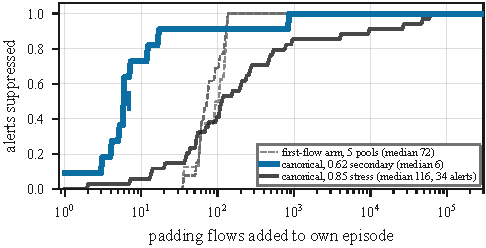
\includegraphics[width=\columnwidth]{figE_padding_sensitivity.pdf}
\caption{The sensitivity arms the body's \cref{fig:attacks} omits: the secondary window under the
canonical order against the known-invalid stress window (canonical) and the five pad pools under
first-flow arrival. Ticks are the five pools' canonical medians at the secondary window, which span
$6$--$7$ flows --- the pad-realism claim of this subsection. Costs move with window, order and pool;
suppressibility does not.}
\label{fig:padsens}
\end{figure}


The realism of the pad barely matters. Generic benign, attacker-origin, protocol-matched and black-box
pools have nearly identical median costs, because the running threshold dwarfs the largest pool mean
e-value ($216.8$); service-matched padding is dearer --- $1.2$--$1.5\times$ under the canonical order,
$1.4$--$2.0\times$ under first-flow, and on a smaller episode subset --- and does not change the
conclusion (\cref{tab:pools}). Under the headline key the adversary sends ordinary traffic between the
source and destination already involved in its activity before the two-hour bucket closes. The flow-only
detector reads no endpoint identity, but 17 of 33 features are backward or bidirectional, so whether a
flow the victim answers transfers is empirical; the real-flow replay measures it rather than assuming
it. Beyond the $3/3$ and $11/11$ canonical suppressions at the primary and secondary windows, the
replay gives $34/34$ canonical at the stress window, and $18/18$, $13/13$ and $72/72$ under first-flow
order; the measured cost equals the closed form on every episode of every arm
(\cref{apptab:w3dilution}).

\emph{The black-box pool and the dilution replay.} The pad flows of \cref{apptab:w3dilution} are real
flows of the black-box pool, selected on network-observable frequency alone: the most common
$(\text{proto},\text{port})$ over the training prefix, which precedes both calibration and deployment
--- no labels, no detector output, no knowledge of the attacker's own traffic. It picks proto 17/port 53 at
both windows, the same service the label-using rule would, and the resulting pool is measured to be 0.0000\% attack-labelled
(an audit, not a selection criterion). The selection rule matters: taking the mode over \emph{all}
window traffic instead picks the attacker's own flood at the stress window, a pool 90\%
attack-labelled that does not dilute. Zero pad fires out of the sampled flows at both windows is
evidence for the structural premise (ordinary victim-service traffic scores like ordinary traffic),
not proof that the firing probability is zero; the Clopper--Pearson bound in the table says how much
that observation leaves open. Both within-bucket orders are attacked. The key-hash rows are the
canonical order the paper reports, under which a pad provably moves no other hypothesis's spending
weight, so the \cref{assump:groupval} argument is clean; the first-flow rows re-run the identical chain
--- same detector, same pool, same pricing --- on the detected set the initial first-flow order
produces, which \cref{apptab:ordering} shows is the largest over the orders we audit. Every detection is
suppressible under both, and the canonical medians reproduce \cref{tab:main}. The canonical
primary-window set is small, so read it as three individually-priced episodes (costs 23, 24, 33 flows)
rather than as a rate; the canonical costs are lower than the first-flow ones because the two orders
detect different episodes at different steps of the level sequence, not because the canonical order is
weaker.


\emph{Residual risk at the horizon-aware arm.} The pool's zero firing count over $845{,}691$ flows is
a fact about the pool, and it leaves open a risk that replay cannot bound --- so we simulate pads
whose flows fire independently at the one-sided $95\%$ Clopper--Pearson upper limit the observation
admits, $p\le3.5\times10^{-6}$. Even there the worst alert suppresses on an estimated $90.5\%$ of
draws at the primary window and $82.5\%$ at the secondary (\cref{sec:replay}). Both figures are Monte
Carlo estimates over $200$ draws and both treat pool flows as independent draws from a common firing
rate, which the pool's composition does not establish.

\subsection{The AIT transfer arms}\label{app:ait}

\emph{Host-conditioned detector on LSPR23.} The detector of \cref{apptab:r7host} reads the 33 flow
features plus 6 strictly causal ($\mathrm{ts}<\mathrm{ts}(\text{flow})$) host-context features ---
per-host prior counts, distinct-peer counts and failed-connection fractions --- and no endpoint ground
truth (\texttt{label\_src} and \texttt{label\_dst} both have attack rate $1.0$ and are excluded). It has
higher AUROC than the flow-only detector at both windows, yet lower tail reach and fewer e-LOND
detections ($2$ against $18$ at the primary window): higher ranking quality buying fewer, not more,
operational alerts, the detector-quality-versus-feasibility gap of \cref{sec:feasnotdet}. To test the
padding boundary we graft each attacked pair's real causal context (strongest feature src-distinct-dst,
$\rho=+0.34$; padding one victim cannot raise it) onto ordinary black-box pads ---
the most common $(\text{proto},\text{port})$ on the training prefix, which precedes both calibration
and deployment, so the pool is chosen on network-observable frequency alone with no labels and no
detector output --- and replay the append causally. The pads fire zero across the scored accumulation
range at both windows --- up to 100{,}000 appended flows per episode, 4{,}000{,}000 pad scorings at the
primary window --- and the suppression cost is the identical flow-level closed form (0.55 $r^{\star}_t=108$ host vs 118 flow; 0.85 $r^{\star}_t=11{,}484$ host vs 5{,}202 flow),
so within that range the transfer holds at both; costs above the cap are closed-form values, not
replayed. A non-black-box pool rule does fire: selecting the modal service among detector-non-firing
flows picks proto 6/port 80 at $0.85$, a pool that is only $12\%$ benign and fires $0.42$. Grafting the attacker's own flood onto attack context and
observing the detector fire is not evidence of a defence, so that rule is reported only as a
sensitivity. What LSPR23 cannot settle is the benign-inclusive question: its attacked pairs are $100\%$
malicious, so no real ordinary-to-victim traffic exists there, which is what the AIT testbed supplies.


Resequencing the flow-only folds by first-flow arrival --- the detector fit, scores, calibration and
e-values are computed before ordering and are identical across the two arms --- gives 84 of 85, and the
canonical alerts are the \emph{cheaper} to suppress: per-organisation median $r^{\star}_{t,\mathrm{emp}}$ falls from
$212$--$13{,}142$ flows under first-flow to $12$--$4{,}650$ under the canonical order
(\cref{apptab:aitorder}). On \texttt{shaw}, ordinary victim traffic fires often in its \emph{own}
context (7\%), which under a static-context replay made no episode suppressible; scored in the attacked
pair's evolving context the same pool fires at most $0.5\%$, and all three targets suppress
(\cref{apptab:r7ait,apptab:aitsupp}). That contrast is why the host-conditioned arm recomputes context
causally rather than scoring the pool in isolation.

\emph{Design of the AIT replay.} Per organisation, \cref{apptab:aitsupp} trains a
leave-one-organisation-out detector whose flow features are chosen per fold from the training
organisations only, calibrates on in-organisation benign flows strictly preceding the first attack,
forms $(\mathrm{SrcIP},\mathrm{DstIP},\text{2\,h})$ episodes, runs e-LOND, and suppresses each detected
malicious episode by replaying real benign flows to an attacked victim of the organisation (200
draws). A firing pad contributes the maximum e-value and raises the cost, which the zero-pad closed form
misses. The two arms replay differently because the two detectors read different things. Flow-only:
flow features carry no context, so pads are drawn with replacement from the pool's observed
$0$-or-$\ceil$ evidence, an empirical i.i.d.\ generator, so a modelled cost may exceed the finite
observed pool. Host-conditioned: the six host features are causal, so appending pads changes the
context every later pad is scored in, and holding them fixed would be a static-context diagnostic
rather than a replay; we therefore recompute the victim's context as pads accumulate (counts raised,
distinct-peer counts pinned, failure fractions moved to the pool's rate), score the whole pool under
it, and report a success only over the accumulation range actually scored. The chain runs end-to-end
at all eight organisations, in both arms: under first-flow order 84 of 85 flow-only detections are
suppressible, per-draw success $0.79$--$1.00$, and 57 of 63 host-conditioned
detections are, per-draw success $0.61$--$1.00$. Host conditioning therefore blunts the attack
without stopping it. The causal replay is what shows both halves. It is why most episodes still
suppress: \texttt{shaw}'s ordinary-to-victim flows fire 7\% in
their own contexts, which under a static-context replay made no episode suppressible, but a pad's
context is the attacked pair's, and under that context the same pool fires at most
0.5\% across accumulation, so all three episodes suppress. It is also why the
remaining 6 do not (\texttt{harrison}, \texttt{wardbeck}, \texttt{wheeler}): under the accumulated context a pad can
itself fire, and a firing pad adds the ceiling to the group's evidence instead of diluting it, so on
those episodes no draw brings the group mean below threshold in any of the 200 draws, within twice
the zero-pad cost (at least $1{,}000$ pads), which is the range the context curve is scored over. What
decides the outcome is the pad count an episode needs against the rate at which pads fire along that
accumulation path. These are censored simulations rather than proof that the episodes cannot be
padded: a budget or a draw count large enough might still find a route. The pinning
models a single already-active attacker--victim pair; padding from new hosts would move the
distinct-peer counts and is not covered.


\emph{The joint attack on AIT.} \Cref{apptab:joint76} re-runs e-LOND over the padded stream for
each organisation, so the controller's rejection count responds to the attack and, on the
host-conditioned arm, every later flow on the attacked pair is re-scored as the pads arrive. Each figure
is the median over 100 pad-sampling trajectories; the totals below sum those medians over the eight
organisations and are not counts from a single run. Two template pools are separated throughout: the
\emph{deployment} pool is the benign-to-victim traffic the per-alert arms of \cref{apptab:aitsupp} use,
and the \emph{prior} pool is restricted to flows the victim had received before the attacker's own last
flow in the episode. An episode whose prior pool holds fewer than 20 flows is never padded.

With the deployment pool the campaign costs 244{,}250 and 91{,}713 flows against per-alert sums of
607{,}802 and 599{,}967, leaving 1 and 0 of the 79 and 80 own alerts. With the prior pool
24 and 27 remain and no organisation is cleared, at 430{,}626 and 242{,}206 flows: 30 of the
95 attacker-owned episodes have too little prior traffic to imitate and 18 have none at all, and those
episodes carry most of what survives. On the host-conditioned arm, \texttt{shaw} issues 3 and 3 own alerts and 1 and 6 non-attacker alerts; the deployment pool clears all of them for 28 and 7 flows, the victim's prior traffic leaves 2 and 2; \texttt{wilson} issues 6 and 6 own alerts and 0 and 0 non-attacker alerts; the deployment pool clears all of them for 73{,}337 and 16{,}975 flows, the victim's prior traffic leaves 1 and 1.

The state-free multiplier $c=\lfloor\rho\rfloor+1$ of \cref{cor:dilution} leaves 65 and 60 alerts standing
with the prior pool. Sizing it on the episode's full arity rather than the attacker's own flow count
changes nothing there (65 and 60), and changes the outcome only with the deployment pool
(57 and 1 against 59 and 6): what the attacker does not know about co-resident benign
flows costs it nothing while cover traffic is the binding constraint.


\subsection{The aggregation defences, measured}\label{app:defences}

Caps large enough to preserve the intended validity domain yield zero detections at the median
window--seed cell (first-flow, the detection-favourable order; \cref{apptab:caps}). In the
primary-window weight sweep every scheme that retains the mean's recall is defeated by one to eight
leading flows, against 111 appended flows for the mean on the same episodes, and buying a larger
$L^{\star}$ costs about $58\%$ of the recall (\cref{tab:asym}). For the group maximum, direct group
calibration replaces $1.8$--$2.4$M calibration flows by $37$--$57$k groups while leaving $T$ essentially
unchanged; by \cref{cor:budget} that is 20 groups per hypothesis the construction cannot supply, so the
margin collapses to about $-0.97$ and the primary and secondary windows issue no alerts
(\cref{sec:groupcal}). Appending is not the only lever against it either: creating hypotheses ahead of a
target pushes it past the cold-start window, and in that construction's short prefix every
group-maximum detection falls to $62$--$295$ inserted hypotheses (\cref{apptab:insertion}).

\emph{Static versus running pricing.} Pricing against the static first-step threshold $T/w_0$ is the
cheap extreme (median 34 flows at 0.85 under the canonical order); the body reports the larger
running-level cost. Whole-detected-set totals are upper bounds, since suppressing an early rejection
lowers $R$ and can make the rest cheaper or moot, and are heavy-tail driven at their extreme.

\emph{Insertion against padding.} Insertion beats padding for one alert at none of the twelve
window--order cells, but silences the entire controller for $217$--$813$ inserted hypotheses against
$80$--$7.9\times10^{8}$ flows to pad every detection separately; per episode the targeted insertion cost
is $434$--$5{,}674$ hypotheses under the canonical and first-flow orders (down to 407 under a keyed hash).
Under a public hash the ranking is an offline search we price at
$1.0\times10^{4}$--$1.8\times10^{5}$ candidate keys, on three stated conditions (a public seed, enough
endpoint pairs the adversary can send between, and a stable key encoding).

\subsection{The joint controller-state rerun}\label{app:joint}

The per-alert costs of \cref{sec:costcurve} price each alert at the level it received on the
unperturbed trajectory. \Cref{apptab:joint} instead propagates the zero-evidence pads that the
real-flow replay of \cref{sec:replay} validates through the controller, which is re-run over the
padded stream, so that its rejection count --- and with it every later level
$\alphat=\alpha\gamma_t(R_{t-1}{+}1)$ --- responds to the attack. The black-box pool contains no flow
that reaches the conformal tail at either window, so this is the zero-evidence limit of the real-flow
replay, not a second replay. Three attackers are run. \emph{Static}: the per-alert oracle pads of
\cref{tab:costcurve}, applied to every true detection at once. \emph{Sequential}: a greedy oracle
that pads each of its own episodes that would fire at the \emph{live} level by the minimum; its total
$J_{\mathrm{seq}}$ is one strategy's cost on this stream, an upper bound on the minimum joint cost
over all attacker-controlled episodes in the window. \emph{State-free}: every own episode is
multiplied by the integer $c_{\mathrm{int}}=\lfloor\rho\rfloor+1$ of \cref{cor:dilution}, which is
$3$ at the primary and $3$ at the secondary
window, and silences the arm with no controller state. With $R=0$ throughout, the stream-specific
boundary is $c_{\mathrm{crit}}=\max_j \Ev_j\,\alpha\gamma_{t_j}\le\ceil\alpha/T=\rho$, with equality
when a malicious episode attains the ceiling, as one does at each window ($c_{\mathrm{crit}}=\rho=2.134$
and $2.485$); rejection is inclusive, so the boundary must be strictly
exceeded, the real-valued checks just above and below $c_{\mathrm{crit}}$ are a continuous relaxation,
and only the integer $c_{\mathrm{int}}$ is a realisable prescription. The lower panel re-runs the sequential attacker under a per-host-pair volume cap $n$:
it pads only if $m_t+r\le n$ and otherwise lets the alert fire and raise $R$, and each surviving alert
is classified as structural or as a cascade victim by whether its pad would have fitted at $R=0$.
Every padded stream was regrouped from flows and asserted against the unperturbed stream on what an
append must leave unchanged --- the episode count, the (source, destination, bucket) key of every
controller position and hence the permutation, each group's first timestamp and its label --- and
asserted to carry arities $m_t+r_t$ and exactly the padded group means $S_t/(m_t+r_t)$ that the
attacker was priced on; the padded means differ from the unperturbed ones by construction.


\begin{table}[t]
\centering
\caption{Five padding pools priced against the \emph{running} e-LOND level $1/\alphat$, detector
seed 0, two-hour grouping, at the secondary window (0.62) and the stress-test window (0.85), under
\textbf{both} within-bucket orders --- the canonical metadata hash \cref{tab:main} reports and the
first-flow arrival order kept as the optimistic upper bound. Entries are the median suppression cost
$r$ per detected episode, over the detected set that order produces (counts in the block headings);
the order changes \emph{which} episodes must be paid for and how deep into the level sequence they
sit, which is why the two blocks differ by more than a constant. Four pools coincide within each
block; service-matched is dearer, both from a larger mean e-value and from being defined on a
costlier episode subset (\cref{sec:paddingcost}). $\mu$ is the pool-level mean e-value at 0.85 where
defined, a property of the pool and not of the order. Protocol- and service-matched use the episode's
modal protocol/port. Costs are lower bounds.}
\label{tab:pools}
\resizebox{\columnwidth}{!}{%
\begin{tabular}{lrrr}
\toprule
Padding pool & $\mu$ (0.85) & median $r$ (0.62) & median $r$ (0.85) \\
\midrule
\multicolumn{4}{l}{\emph{canonical metadata-hash order (headline)} --- $11$ detected at $0.62$, $34$ at $0.85$} \\
generic benign & 50.9 & $6$ & $116$ \\
attacker-origin & 216.8 & $6$ & $116$ \\
protocol-matched & --- & $6$ & $116$ \\
service-matched & --- & $7$ & $175$ \\
black-box & \textbf{0.0} & $6$ & \textbf{$116$} \\
\midrule
\multicolumn{4}{l}{\emph{first-flow arrival (optimistic upper bound)} --- $13$ detected at $0.62$, $72$ at $0.85$} \\
generic benign & 50.9 & $72$ & $5{,}212$ \\
attacker-origin & 216.8 & $72$ & $5{,}247$ \\
protocol-matched & --- & $72$ & $5{,}232$ \\
service-matched & --- & $99$ & $10{,}299$ \\
black-box & \textbf{0.0} & $72$ & \textbf{$5{,}202$} \\
\bottomrule
\end{tabular}}
\end{table}

\begin{table}[t]
\centering
\caption{Padding suppression cost priced against the running controller level $1/\alphat$
(real) vs the static $T/w_0$ threshold. Part (a) gives \emph{both} within-bucket orders at both
detector seeds: the \textbf{canonical} metadata-hash order the paper reports, and the first-flow
arrival order retained as an optimistic upper bound over the orders we audit (\cref{apptab:ordering}).
Detections and the level an alert fires at both move with the order; $T$, $\nCal$, AUROC and the
margin do not. Part (b)'s pool comparison is on the first-flow detected set, the larger of the two;
\cref{tab:pools} gives the same comparison under \emph{both} orders.
Four pools coincide; service-matched is dearer. Medians are rounded to the nearest integer; ``--''
marks a window/seed/order with no detections.}
\label{apptab:padpools}
\resizebox{\columnwidth}{!}{%
\begin{tabular}{rr rrr rrr}
\toprule
\multicolumn{8}{c}{(a) per window $\times$ seed $\times$ order (e-LOND poly, two-hour grouping)} \\
\midrule
& & \multicolumn{3}{c}{\textbf{canonical key-hash}} & \multicolumn{3}{c}{first-flow (upper bd.)} \\
\cmidrule(lr){3-5}\cmidrule(lr){6-8}
pos & seed & det. & pad (real) & pad (static) & det. & pad (real) & pad (static) \\
\midrule
0.55 & 0 & 3 & 24 & 3 & 18 & 118 & 4 \\
0.55 & 1 & 2 & 27 & 2 & 18 & 101 & 3 \\
0.62 & 0 & 11 & 6 & 4 & 13 & 72 & 4 \\
0.62 & 1 & 8 & 5 & 2 & 12 & 69 & 0 \\
0.70 & 0 & 0 & -- & -- & 30 & 1,851 & 62 \\
0.70 & 1 & 0 & -- & -- & 0 & -- & -- \\
0.77 & 0 & 0 & -- & -- & 31 & 1,165 & 85 \\
0.77 & 1 & 0 & -- & -- & 31 & 1,289 & 90 \\
0.85 & 0 & 34 & 116 & 34 & 72 & 5,202 & 33 \\
0.85 & 1 & 32 & 109 & 34 & 71 & 6,802 & 33 \\
\bottomrule
\end{tabular}}

\vspace{4pt}
\begin{tabular}{lrrr}
\toprule
\multicolumn{4}{c}{(b) five padding pools, seed 0 (median suppression cost $r$)} \\
\midrule
padding pool & real (0.62) & real (0.85) & static (0.85) \\
\midrule
generic benign & 72 & 5,212 & 33 \\
attacker-origin & 72 & 5,247 & 33 \\
protocol-matched & 72 & 5,232 & 33 \\
service-matched & 99 & 10,299 & 35 \\
black-box & 72 & 5,202 & 33 \\
\bottomrule
\end{tabular}
\end{table}

\begin{table}[t]
\centering
\caption{Controlled padding-dilution replay on the shipped detector: real flows of the black-box pool
appended to every detected episode under both within-bucket orders (\textbf{canonical} key-hash and
\textbf{first-flow}); src--dst two-hour unit, e-LOND $\gamma\propto j^{-1.6}$, seed 0. Design and
reading: \cref{app:pools}.}
\label{apptab:w3dilution}
\resizebox{\columnwidth}{!}{%
\begin{tabular}{llrrrrrr}
\toprule
window & within-bucket order & pool flows & pad fires & $95\%$ upper & detected & measured $=$ c.f.\ & median $r^{\star}_t$ \\
\midrule
primary (0.55) & first-flow \emph{(upper bd.)} & 845,691 & 0/20,000 & $1.5\times10^{-4}$ & 18 & 18/18 & 118 \\
 & \textbf{key-hash (canonical)} & 845,691 & 0/20,000 & $1.5\times10^{-4}$ & 3 & 3/3 & 24 \\
stress-test (0.85) & first-flow \emph{(upper bd.)} & 584,850 & 0/20,000 & $1.5\times10^{-4}$ & 72 & 72/72 & 5{,}202 \\
 & \textbf{key-hash (canonical)} & 584,850 & 0/20,000 & $1.5\times10^{-4}$ & 34 & 34/34 & 116 \\
\bottomrule
\end{tabular}}
\par\vspace{3pt}
{\footnotesize\raggedright \emph{Notes.} ``pool flows'': the black-box pool's size in the window;
``pad fires'': how many of $n$ sampled pad flows fire when run through the detector, with the exact
one-sided $95\%$ Clopper--Pearson upper bound on the firing probability in the next column;
``measured $=$ c.f.'': detected episodes whose padded group e-value $S_t/(m_t+r)$ crosses the firing
threshold at exactly the predicted $r^{\star}_t=\lfloor S_t\alphat\rfloor-m_t+1$; ``median
$r^{\star}_t$'': over the detected episodes of the row, priced at the running level.\par}
\end{table}

\begin{table}[t]
\centering
\caption{Surface~A priced \textbf{without oracle state}: a re-analysis of the same per-episode
$(m,S,\alphat)$ the oracle costs come from, with no re-simulation --- the closed form \eqref{eq:rstar} is re-derived from the stored fields on all 127
episodes as a read-back check. \emph{Multiplier}: append $(c-1)m$ flows, that is, multiply your own
episode by $c$. It defeats the alert iff $c\ge1+r^{\star}_t/m_t$ and needs \textbf{no} estimate of $S_t$,
$\alphat$ or $\nCal$ --- only $m$, which on LSPR23 is the attacker's own flow count, since every host
pair carrying attack traffic is 100\% malicious. ``padded arity'' is $cm$, and the column beside it answers
the deployment-side question --- would a volume monitor see the pad --- as the fraction of
\emph{deployment} episodes larger than the padded one, bracketed by the two stored group-size quantiles
that straddle it. Those quantiles are \emph{not} shown and are \emph{not} benign deployment values:
they are quantiles of source--destination group size over the \emph{calibration} slice, unfiltered by
label, which is why the deployment exceedance and not the quantile is what the claim rests on. Rows are given under \textbf{both}
within-bucket orders --- the \textbf{canonical} metadata hash the paper reports and \textbf{first-flow}
arrival, retained as the optimistic upper bound. \emph{Absolute}: append a
pre-committed flat $N$ flows, which needs nothing at all; $N$ is reported at the fraction of that
cell's alerts it suppresses. The multiplier arm covers the two windows for which per-episode arities
are stored; the secondary window appears in the absolute arm only. Both strategies are upper bounds
on the oracle cost, and both are optimistic on a benign-inclusive stream, where $m$ also contains
benign flows the attacker cannot see.}
\label{apptab:nonoracle}
\resizebox{\columnwidth}{!}{%
\begin{tabular}{llrrrrrrrr}
\toprule
\multicolumn{10}{l}{\emph{multiplier --- needs the attacker's own arity $m$ and nothing else}} \\
order & pos & alerts & med.\ $c$ & max $c$ & $c$ used & med.\ added & vs oracle & padded arity & \% deployment larger \\
\midrule
canonical & 0.55 & 3 & 1.57 & 2.74 & 3 & 80 & 3.5$\times$ & 120 & 0.9--9.9\% \\
canonical & 0.85 & 34 & 2.76 & 6.17 & 10 & 792 & 5.1$\times$ & 880 & 0.1--1.1\% \\
first-flow & 0.55 & 18 & 3.54 & 7.44 & 10 & 414 & 3.6$\times$ & 460 & 0.1--0.9\% \\
first-flow & 0.85 & 72 & 73.19 & 4302.15 & \emph{none $\le$ 100} & --- & --- & --- & --- \\
\bottomrule
\end{tabular}}

\vspace{3pt}
\resizebox{\columnwidth}{!}{%
\begin{tabular}{llrrrrr}
\toprule
\multicolumn{7}{l}{\emph{absolute --- a flat pad: executing it needs no state, but the $N$ below is read off the realised $r^{\star}_t$ distribution}} \\
order & pos & seed & alerts & $N$ for 50\% & $N$ for 90\% & $N$ for all \\
\midrule
canonical & 0.55 & 0 & 3 & 24 & 33 & 33 \\
canonical & 0.55 & 1 & 2 & 30 & 30 & 30 \\
canonical & 0.62 & 0 & 11 & 6 & 17 & 859 \\
canonical & 0.62 & 1 & 8 & 6 & 659 & 659 \\
canonical & 0.85 & 0 & 34 & 118 & 9{,}395 & 58{,}616 \\
canonical & 0.85 & 1 & 32 & 111 & 9{,}426 & 58{,}620 \\
first-flow & 0.55 & 0 & 18 & 125 & 645 & 837 \\
first-flow & 0.55 & 1 & 18 & 108 & 645 & 829 \\
first-flow & 0.62 & 0 & 13 & 72 & 127 & 134 \\
first-flow & 0.62 & 1 & 12 & 70 & 93 & 98 \\
first-flow & 0.77 & 0 & 31 & 1{,}165 & 3{,}736 & 7{,}886 \\
first-flow & 0.77 & 1 & 31 & 1{,}289 & 4{,}258 & 7{,}886 \\
first-flow & 0.70 & 0 & 30 & 1{,}877 & 4{,}145 & 5{,}445 \\
first-flow & 0.85 & 0 & 72 & 6{,}714 & 69{,}195{,}773 & 145{,}525{,}527 \\
first-flow & 0.85 & 1 & 71 & 6{,}802 & 69{,}086{,}348 & 145{,}096{,}310 \\
\bottomrule
\end{tabular}}
\end{table}


\begin{table}[t]
\centering
\caption{Pre-committed weight schemes at the primary window, LOND, $\gamma \propto j^{-1.6}$, mean over
two detector seeds. $T = 57{,}368$ episodes, 275 malicious, $\nCal = 2{,}448{,}993$. $L^{*}$ is quoted at
the unperturbed level and is therefore an upper bound. All counts here use the \textbf{first-flow}
within-bucket order, the optimistic upper bound over the orders we audit, not the canonical
metadata-hash order \cref{tab:main} reports (\cref{apptab:ordering}); both legs of every comparison use
it, so the order moves the level and not the ranking.}
\label{tab:asym}
\resizebox{\columnwidth}{!}{%
\begin{tabular}{lccrrr}
\toprule
Rule & pad-inv. & recall & $L^{*}$ & appended & ratio \\
\midrule
arithmetic mean (symmetric) & --- & 0.065 & --- & --- & --- \\
first-event-only          & yes & 0.062 & \textbf{1}   & 111 & $112\times$ \\
exp-decay $\rho = 0.5$    & yes & 0.062 & 2   & 111 & $56\times$ \\
uniform over 10 slots     & yes & 0.062 & 8   & 111 & $14\times$ \\
uniform over 100 slots    & yes & 0.027 & 81  & 492 & $6\times$ \\
exp-decay $\rho = 0.99$   & yes & 0.027 & 164 & 492 & $3\times$ \\
last-event-only           & \textbf{no} & 0.045 & --- & 336 & --- \\
security-prior \emph{(out of class)} & yes & 0.000 & --- & --- & --- \\
\bottomrule
\end{tabular}}
\end{table}

\begin{table}[t]
\centering
\caption{Aggregation-cap sweep (median over five positions $\times$ two seeds): the frozen
$n_0=p_{99}$ is chosen for validity and attack cost, not power. ``\% groups $m>n_0$'' is the
share of groups whose size exceeds the cap; ``front-load cost'' is the number of appended
flows needed to defeat the front-loading defence. All counts here use the \textbf{first-flow} within-bucket order, the optimistic upper bound over the orders we audit, not the canonical metadata-hash order \cref{tab:main} reports (\cref{apptab:ordering}); the order shifts detections and the level an alert fires at, and shifts nothing else.}
\label{apptab:caps}
\resizebox{\columnwidth}{!}{%
\begin{tabular}{lrrrrr}
\toprule
cap & $n_0$ & \% groups $m>n_0$ & det.\ raw & det.\ trunc.\ & front-load cost \\
\midrule
mean & 47 & 5.72 & 39.5 & 35 & 16 \\
p50 & 2 & 37.58 & 99 & 71 & 1 \\
p90 & 21 & 10.24 & 68.5 & 60 & 8 \\
p99 & 408 & 1.08 & 0 & 0 & 116 \\
p999 & 7,258 & 0.12 & 0 & 0 & 3,560 \\
max & 97,911 & 0.01 & 0 & 0 & -- \\
\bottomrule
\end{tabular}}
\end{table}

\begin{table}[t]
\centering
\caption{\textbf{Suppression by insertion, not by padding.} \Cref{thm:padding} and every cost in
\cref{sec:paddingcost} concern \emph{appending} flows to a fixed hypothesis. This attack appends
nothing: it \emph{creates} hypotheses ahead of the target, pushing it out of the cold-start window
past which no rejection is possible. Two models are kept apart because they are different attacks.
\textbf{Targeted} inserts only immediately ahead of one episode, which leaves every earlier
hypothesis and hence $R$ untouched, so its cost is closed-form
$G^\star=\lfloor(\alpha(R{+}1)E/\zeta(1.6))^{1/1.6}\rfloor-p$ (replay-verified).
\textbf{Window} inserts ahead of everything and silences the controller outright --- that is
\emph{not} a per-episode cost, since it also deletes the earlier detections that raised $R$.
\textbf{The split verdict is the result:} insertion does \emph{not} beat padding for one alert
(0/12 cells),
but silences the whole window for a few hundred hypotheses
(10/12
cells at one flow per inserted group, 7/12 at two). Padding totals are \textbf{upper} bounds --- the
joint cost is lower, because suppressing an early rejection lowers $R$ --- and the largest ratio is
heavy-tail driven. Panel (b) is the construction of \cref{sec:groupcal}, which padding provably
cannot suppress: calibrating on \emph{groups} shrinks the ceiling, so its cold-start window collapses
to 65--86 and every detection
falls to a few dozen insertions. \emph{Group validity by design plus padding robustness does not buy
attack resistance.} Getting ahead of a target is free under first-flow arrival (send earlier in the
bucket), costs an offline keyspace search under a public hash, and cannot be ranked offline at all
under a keyed one --- which removes the \emph{search}, not the attack. Both within-bucket orders are reported: the \textbf{canonical} metadata key-hash
\cref{tab:main} uses, and \textbf{first-flow} arrival, the optimistic upper bound over the orders we
audit (\cref{apptab:ordering}).}
\label{apptab:insertion}
\resizebox{\columnwidth}{!}{%
\begin{tabular}{rlr rr rr c}
\toprule
\multicolumn{8}{c}{(a) the shipped flow-level pipeline} \\
\midrule
 & & & \multicolumn{2}{c}{per episode} & \multicolumn{2}{c}{silence the window} & \\
\cmidrule(lr){4-5}\cmidrule(lr){6-7}
pos & order & det. & insert & pad (flows) & insert & pad (upper) & cheaper \\
\midrule
0.55 & key-hash & 3 & 434 & 24.0 & 217 & 80 & -- \\
0.55 & first-flow & 18 & 1,696 & 118.0 & 502 & 4,432 & $\checkmark$ \\
0.62 & key-hash & 11 & 605 & 6.0 & 813 & 926 & $\checkmark$ \\
0.62 & keyed & 6 & 452 & 14.5 & 506 & 126 & -- \\
0.62 & first-flow & 13 & 2,284 & 72.0 & 554 & 1,060 & $\checkmark$ \\
0.70 & keyed & 3 & 407 & 97.0 & 257 & 310 & $\checkmark$ \\
0.70 & first-flow & 30 & 4,088 & 1,850.5 & 706 & 62,250 & $\checkmark$ \\
0.77 & keyed & 3 & 556 & 323.0 & 416 & 1,205 & $\checkmark$ \\
0.77 & first-flow & 31 & 3,161 & 1,165.0 & 789 & 49,957 & $\checkmark$ \\
0.85 & key-hash & 34 & 1,414 & 115.5 & 509 & 151,390 & $\checkmark$ \\
0.85 & keyed & 24 & 998 & 160.5 & 518 & 162,496 & $\checkmark$ \\
0.85 & first-flow & 72 & 5,674 & 5,201.5 & 743 & 786,257,264 & $\checkmark$ \\
\bottomrule
\end{tabular}}

\vspace{4pt}
\resizebox{\columnwidth}{!}{%
\begin{tabular}{rrrrrrr}
\toprule
\multicolumn{7}{c}{(b) the group-calibrated \textsc{max} pipeline --- padding cannot suppress it at all} \\
\midrule
pos & groups & firing & detections & cold start & targeted $G^\star$ & window $G$ \\
\midrule
0.55 & 57,368 & 110 & 0 & 81 & -- & -- \\
0.62 & 49,267 & 109 & 0 & 83 & -- & -- \\
0.70 & 37,231 & 69 & 1 & 86 & 81.0 & 81 \\
0.77 & 31,672 & 60 & 2 & 78 & 76.5 & 68 \\
0.85 & 31,568 & 152 & 42 & 65 & 207.0 & 62 \\
\bottomrule
\end{tabular}}
\end{table}

\begin{table}[t]
\centering
\caption{Host-conditioned detector and the padding-transfer boundary on LSPR23 (src--dst two-hour
unit, e-LOND $\gamma\propto j^{-1.6}$, seed 0; \textbf{first-flow} within-bucket order on both legs,
the optimistic upper bound over the orders we audit, not the canonical order \cref{tab:main} reports).
``h/f'': host-conditioned / flow-only detector. Design and reading: \cref{app:ait}.}
\label{apptab:r7host}
\resizebox{\columnwidth}{!}{%
\begin{tabular}{lcccrrrc}
\toprule
window & AUROC h/f & tail reach h/f & det.\ h/f & real benign fires & graft fire & median cost h/f & transfer \\
\midrule
primary (0.55) & 0.954/0.916 & 0.009/0.033 & 2/18 & $0/2{,}287{,}988$ & $0.000$ & 108/118 & holds \\
stress-test (0.85) & 1.000/0.999 & 0.295/0.610 & 37/72 & $3/1{,}638{,}722$ & $0.000$ & 11{,}484/5{,}202 & holds \\
\bottomrule
\end{tabular}}
\par\vspace{3pt}
{\footnotesize\raggedright \emph{Notes.} ``AUROC'': area under the ROC curve on the window's flows;
``tail reach'': the fraction of attack flows scoring above every benign calibration score; ``det.'': e-LOND detections; ``real benign fires'': host-detector firings among
the window's benign flows; ``graft fire'': the grafted-pad firing rate on detected episodes across
accumulation; ``median cost h/f'': the median suppression cost over detected episodes under the causally
recomputed host context / the flow-level closed form $r^{\star}_t$; ``transfer'': whether the flow-level closed form still prices the suppression. All counts here use the \textbf{first-flow} within-bucket order, the optimistic upper bound over the orders we audit, not the canonical metadata-hash order \cref{tab:main} reports (\cref{apptab:ordering}); the order shifts detections and the level an alert fires at, and shifts nothing else.\par}
\end{table}

\begin{table}[t]
\centering
\caption{The padding-transfer boundary re-measured on a \emph{benign-inclusive} testbed
(AIT-LDSv2.0, \textbf{8} organisations,
\textbf{45{,}001} attack flows), where victims serve
heavy real benign traffic while attacked, so the padding question is answered on \emph{real}
ordinary-to-victim flows --- \textbf{no graft}. Leave-one-organisation-out (train 7, test 1; a
``deploy on a new network'' test), in-organisation benign conformal calibration, flow features
selected per fold from the training orgs with all identity and \emph{absolute-time} fields excluded.
``benign$\to$victim'' is the fire rate of real benign flows to an attacked host (the pad analogue),
host\,/\,flow-only. Host conditioning adds little and inconsistently (median host$-$flow delta
$-0.0000$; host higher on $1/8$ orgs, max $8.9\%$),
with \texttt{shaw} the one organisation where it is materially higher.
\textbf{That per-organisation exception is real but does not survive as a defence.} A raised
ordinary-to-victim fire rate is measured here \emph{in each flow's own context}; the pads an attacker
actually sends carry the \emph{attacked} pair's context, and replaying the whole Surface~A chain under
that context suppresses every detected Shaw episode (\cref{apptab:aitsupp}). So the honest reading is
that host conditioning is usually negligible here and can look decisive on an individual organisation,
but replaying the chain end-to-end at all eight organisations it does not stop the attack on most
episodes once the pad's own context is modelled, and where it does the binding constraint is the
number of pads required (\cref{apptab:aitsupp}). This also settles the LSPR23 side: the $0.43$ grafted firing at the
stress window comes from a non-black-box pad pool that is mostly the attacker's own flood
(\cref{apptab:r7host}). AIT has no high-volume flood, which remains open. The flow-only folds are audited under \textbf{both} within-bucket orders in
\cref{apptab:aitorder}: the canonical order detects fewer episodes and its alerts are cheaper to
suppress, as on LSPR23. Rows sequenced by \textbf{first-flow} arrival are conditional on the detected
set that order produces on this testbed.}
\label{apptab:r7ait}
\resizebox{\columnwidth}{!}{%
\begin{tabular}{lccc}
\toprule
organisation & AUROC h/f & atk.\ recall & benign$\to$victim \% (h/f) \\
\midrule
\texttt{fox} & 0.995/0.996 & 0.93 & 0.00/0.01 \\
\texttt{harrison} & 0.975/0.973 & 0.86 & 0.01/0.01 \\
\texttt{russellmit} & 0.988/1.000 & 0.47 & 0.00/0.02 \\
\texttt{santos} & 0.948/0.980 & 0.36 & 0.00/0.01 \\
\texttt{shaw} & 0.955/0.932 & 0.47 & 8.92/0.05 \\
\texttt{wardbeck} & 0.969/0.907 & 0.39 & 0.14/0.01 \\
\texttt{wheeler} & 0.999/0.998 & 0.97 & 0.01/0.01 \\
\texttt{wilson} & 0.974/0.984 & 0.85 & 0.07/0.00 \\
\bottomrule
\end{tabular}}
\end{table}

\begin{table}[t]
\centering
\caption{Full suppression pipeline on the benign-inclusive AIT testbed: per organisation, a
leave-one-organisation-out detector, in-organisation benign calibration preceding the first attack,
two-hour host-pair episodes, e-LOND, and each detected malicious episode suppressed by replaying real
ordinary-to-victim flows against the running controller level (200 draws). Rows are sequenced by
\textbf{first-flow} arrival and are conditional on the detected set that order produces; the flow-only
folds under both orders are \cref{apptab:aitorder}. Design and reading: \cref{app:ait}.}
\label{apptab:aitsupp}
\resizebox{\columnwidth}{!}{%
\begin{tabular}{lrrrrrr}
\toprule
org & det. & pad fire & $r^{\star}_{t,\mathrm{emp}}$ & $r^{\star}_t$ (closed) & suppr. & succ. \\
\midrule
\multicolumn{7}{l}{\emph{flow-only detector}} \\
fox & 13/14 & 1.3e-04 & 277 & 277 & 13/13 & 1.00 \\
harrison & 10/14 & 1.8e-04 & 1{,}412.5 & 1{,}412.5 & 10/10 & 1.00 \\
russellmitchell & 14/14 & 5.2e-04 & 3{,}551.5 & 3{,}365.5 & 14/14 & 0.97 \\
santos & 9/9 & 4.7e-04 & 212 & 212 & 8/9 & 0.79 \\
shaw & 3/6 & 0.0e+00 & 404 & 404 & 3/3 & 1.00 \\
wardbeck & 9/9 & 3.2e-04 & 13{,}142 & 8{,}294 & 9/9 & 0.90 \\
wheeler & 15/16 & 2.1e-04 & 1{,}609 & 1{,}609 & 15/15 & 1.00 \\
wilson & 12/13 & 4.3e-05 & 793 & 793 & 12/12 & 1.00 \\
\midrule
\multicolumn{7}{l}{\emph{host-conditioned detector, end-to-end}} \\
fox & 9/14 & 0.0e+00 & 115 & 55 & 9/9 & 1.00 \\
harrison & 7/14 & 2.9e-04 & 792.5 & 692 & 6/7 & 0.86 \\
russellmitchell & 9/14 & 0.0e+00 & 1{,}140 & 1{,}140 & 9/9 & 1.00 \\
santos & 5/9 & 0.0e+00 & 43 & 43 & 5/5 & 1.00 \\
shaw & 3/6 & 7.0e-02 & 269 & 269 & 3/3 & 1.00 \\
wardbeck & 9/9 & 1.3e-03 & 8{,}471.5 & 8{,}263.5 & 8/9 & 0.74 \\
wheeler & 15/16 & 3.6e-04 & 1{,}609 & 1{,}486 & 11/15 & 0.61 \\
wilson & 6/13 & 0.0e+00 & 355 & 355 & 6/6 & 1.00 \\
\bottomrule
\end{tabular}}
\par\vspace{3pt}
{\footnotesize\raggedright \emph{Notes.} ``det.'': e-LOND true detections over malicious episodes; ``pad
fire'': the real ordinary-to-victim firing rate as observed; ``$r^{\star}_{t,\mathrm{emp}}$'': the empirical median
replay cost over suppressible episodes; ``$r^{\star}_t$ (closed)'': the zero-pad closed-form lower bound over
the same episodes ($\le$ empirical by construction); ``suppr.'': detected episodes for which at least
one of the 200 draws brought the group below threshold inside the scored range --- a
possibility count, not a reliability one; ``succ.'': the mean per-draw success, which is the
reliability the count does not carry. An episode outside ``suppr.'' had no successful draw within that
budget, which does not establish that it cannot be padded.\par}
\end{table}

\begin{table}[t]
\centering
\caption{The AIT transfer under \textbf{both} within-bucket orders, flow-only folds. This is a
\emph{resequencing}: the leave-one-organisation-out feature selection, the per-fold detector fit, the
scores, the chronological in-organisation calibration and the e-values are all computed before
episodes are ordered, so the two arms differ by the permutation alone; the canonical arm uses the same
key-hash rule as the LSPR23 results. The stored first-flow arm is re-derived here as a read-back
check that this is the same chain and not merely a similar one (it reproduces 84/85). The
canonical order detects fewer episodes, as on LSPR23, and the alerts it does issue are
\emph{cheaper} to suppress --- per-organisation median $r^{\star}_{t,\mathrm{emp}}$ falls from 212--13142 to 12--4650 flows. The
host-conditioned arm runs at all eight organisations and is left on first-flow
(\cref{apptab:r7ait}). ``det./mal.'' counts \emph{true} detections against malicious episodes;
the eight per-organisation runs issue 83 rejections under the canonical order and 89 under first-flow, carrying 4 and 4 false discoveries
respectively (pooled realised $\FDP$ 0.048 and 0.045); costs are empirical replay medians
$r^{\star}_{t,\mathrm{emp}}$, at or above the zero-pad lower bound $r^{\star}_t$ (\cref{apptab:aitsupp}
lists both for the first-flow arm).}
\label{apptab:aitorder}
\resizebox{\columnwidth}{!}{%
\begin{tabular}{lrrrr}
\toprule
organisation & det./mal. & median $r^{\star}_{t,\mathrm{emp}}$ & suppressible & per-draw succ. \\
\midrule
\multicolumn{5}{l}{\emph{canonical order} --- 78/79 suppressible} \\
\texttt{fox} & 11/14 & 12 & 11/11 & 1.00 \\
\texttt{harrison} & 9/14 & 50 & 9/9 & 1.00 \\
\texttt{russellmitchell} & 14/14 & 4{,}650 & 13/14 & 0.93 \\
\texttt{santos} & 8/9 & 35.5 & 8/8 & 1.00 \\
\texttt{shaw} & 3/6 & 26 & 3/3 & 1.00 \\
\texttt{wardbeck} & 8/9 & 65 & 8/8 & 1.00 \\
\texttt{wheeler} & 15/16 & 192 & 15/15 & 1.00 \\
\texttt{wilson} & 11/13 & 274 & 11/11 & 1.00 \\
\midrule
\multicolumn{5}{l}{\emph{first-flow order} --- 84/85 suppressible} \\
\texttt{fox} & 13/14 & 277 & 13/13 & 1.00 \\
\texttt{harrison} & 10/14 & 1412.5 & 10/10 & 1.00 \\
\texttt{russellmitchell} & 14/14 & 3551.5 & 14/14 & 0.97 \\
\texttt{santos} & 9/9 & 212 & 8/9 & 0.79 \\
\texttt{shaw} & 3/6 & 404 & 3/3 & 1.00 \\
\texttt{wardbeck} & 9/9 & 13{,}142 & 9/9 & 0.90 \\
\texttt{wheeler} & 15/16 & 1{,}609 & 15/15 & 1.00 \\
\texttt{wilson} & 12/13 & 793 & 12/12 & 1.00 \\
\bottomrule
\end{tabular}}
\end{table}

\begin{table*}[t]
\centering
\caption{Joint attack on the benign-inclusive AIT stream, flow-only detector, canonical order, seed 0,
medians over 100 pad-sampling trajectories. ``own'' and ``other'' are the baseline alerts on
attacker-owned and other episodes, horizon-free/horizon-aware. ``no pool'' counts own episodes whose
prior traffic to the victim is under 20 flows. For each spending rule the attacker is run twice: from the
\emph{deployment} pool the per-alert arms use, and from the victim's \emph{prior} traffic only; each pair
of columns gives the alerts still standing and the flows spent. Reading and the host-conditioned arm:
\cref{app:ait}.}
\label{apptab:joint76}
\footnotesize
\setlength{\tabcolsep}{4pt}
\begin{tabular}{lcccrrrrrrrr}
\toprule
& & & & \multicolumn{4}{c}{horizon-free} & \multicolumn{4}{c}{horizon-aware} \\
\cmidrule(lr){5-8}\cmidrule(lr){9-12}
& & & & \multicolumn{2}{c}{deployment} & \multicolumn{2}{c}{prior} & \multicolumn{2}{c}{deployment} & \multicolumn{2}{c}{prior} \\
\cmidrule(lr){5-6}\cmidrule(lr){7-8}\cmidrule(lr){9-10}\cmidrule(lr){11-12}
org & own & other & no pool & left & flows & left & flows & left & flows & left & flows \\
\midrule
fox & 11/11 & 0/0 & 4/14 & 0 & 972 & 2 & 601 & 0 & 5{,}610 & 3 & 61{,}704 \\
harrison & 9/9 & 0/0 & 5/14 & 0 & 4{,}144 & 3 & 11{,}624 & 0 & 21{,}741 & 3 & 69{,}940 \\
russellmitchell & 14/14 & 1/1 & 4/14 & 1 & 68{,}638 & 4 & 157{,}922 & 0 & 5{,}433 & 4 & 8{,}677 \\
santos & 8/9 & 0/1 & 4/9 & 0 & 397 & 4 & 2{,}718 & 0 & 2{,}003 & 6 & 4{,}267 \\
shaw & 3/3 & 3/3 & 4/6 & 0 & 536 & 2 & 906 & 0 & 353 & 2 & 659 \\
wardbeck & 8/8 & 0/0 & 3/9 & 0 & 225 & 3 & 550 & 0 & 4{,}728 & 4 & 15{,}198 \\
wheeler & 15/15 & 0/0 & 2/16 & 0 & 93{,}221 & 1 & 93{,}830 & 0 & 32{,}676 & 1 & 33{,}121 \\
wilson & 11/11 & 0/0 & 4/13 & 0 & 76{,}116 & 5 & 162{,}476 & 0 & 19{,}169 & 4 & 48{,}641 \\
\bottomrule
\end{tabular}
\end{table*}

\begin{table}[t]
\centering
\caption{Both attacks in operational units (position 0.85 --- the \textbf{known-invalid} stress
window; these are attack \emph{costs}, which are measured against the controller's level and do not
rest on the evidence being a valid e-value --- black-box padding pool). Wire
bytes are the per-flow median; rate is priced over the relevant span (7200\,s window for
padding, the position's own deployment span for the state attack). ``$\times$ window'' and
``$\times$ dataset'' are flow-count ratios. \textbf{Each padding row names the procedure whose
level it is priced against, whether that level is the \emph{running} $1/\alphat$ at the episode's own
step or the \emph{static} cold-start $\tau$, and the detected set it is summed over}, because these
differ by two orders of magnitude and are easily confused, \textbf{and the within-bucket order the
detected set was produced under}. Row 1 is the headline cost: the median over e-LOND's own $34$
detections at $0.85$ under the \textbf{canonical} order, priced at the running level --- the value
\cref{tab:main} quotes. Row 2 is the same quantity over the $72$ detections of the
\textbf{first-flow} arrival order, the optimistic upper bound over the orders we audit; it is
$45\times$ dearer because that order detects more episodes and detects them deeper into the level
sequence, where $1/\alphat$ is larger. Both appear in \cref{apptab:padpools}. Rows 3--4 are the \emph{cheap extreme}: $r_{90}$ over the
$257$ episodes of positions $0.62$ and $0.85$ (two seeds) at which all five pools are defined, priced
against the static level-$w_0$ threshold $T/w_0$, first-flow. Row 5 multiplies that static median by
\emph{ADDIS's} $147$-episode detected set (\cref{apptab:addisstate}), so it mixes an e-LOND-scale
per-episode cost with an ADDIS-scale count; it is the cheapest reading of ``suppress everything'' and
is reported only for contrast with the last two rows. Every row below the first is under first-flow
arrival.}
\label{apptab:units}
\resizebox{\columnwidth}{!}{%
\begin{tabular}{lrrrrr}
\toprule
attack budget & flows & wire bytes & rate & $\times$ window & $\times$ dataset \\
\midrule
\textbf{e-LOND, \emph{running} $1/\alphat$: one alert (median), \emph{canonical}} & $116$ & 45.5\,KB & 50.5\,bit/s & $4.7\times10^{-5}$ & $7.1\times10^{-6}$ \\
\quad same, \emph{first-flow} (optimistic upper bd.) & $5{,}202$ & 2.0\,MB & 2265.8\,bit/s & $2.1\times10^{-3}$ & $3.2\times10^{-4}$ \\
level-$w_0$ \emph{static} $\tau{=}T/w_0$: one alert (median) & $34$ & 13.3\,KB & 14.8\,bit/s & $1.4\times10^{-5}$ & $2.1\times10^{-6}$ \\
level-$w_0$ \emph{static} $\tau{=}T/w_0$: one alert (p90) & $227$ & 89.0\,KB & 98.9\,bit/s & $9.3\times10^{-5}$ & $1.4\times10^{-5}$ \\
static median $\times$ ADDIS's 147 detections \emph{(mixed)} & $4{,}998$ & 2.0\,MB & 2176.9\,bit/s & $2.0\times10^{-3}$ & $3.1\times10^{-4}$ \\
ADDIS, \emph{running} $1/\alphat$: one episode (median) & $34{,}465{,}311$ & 13.5\,GB & 15.0\,Mbit/s & $14.05\times$ & $2.11\times$ \\
ADDIS spending-state attack ($B^\ast$ precursors) & $92{,}015{,}637$ & 36.1\,GB & 33.4\,Mbit/s & $37.51\times$ & $5.63\times$ \\
\bottomrule
\end{tabular}}
\end{table}

\begin{table}[t]
\centering
\caption{Joint zero-evidence controller-state rerun: LSPR23, detector seed 0, \textbf{canonical}
order, two-hour host-pair episodes, e-LOND, both windows and both spending regimes. Upper panel: the
static, sequential and state-free attackers of \cref{sec:costcurve}; lower panel: the per-host-pair
volume cap against the sequential attacker. Design and reading: \cref{app:joint}.}
\label{apptab:joint}
\resizebox{\columnwidth}{!}{%
\begin{tabular}{llrrrrrrrrr}
\toprule
window & regime & true det.\ (FD) & median $r^{\star}_t$ / $\sum_{t\in\mathcal D} r^{\star}_t$ & static: remain & $J_{\mathrm{seq}}$ ($\div$ $\sum_{t\in\mathcal D} r^{\star}_t$) & med.\ pad (padded) & spared & padded arity (per-alert) & \% episodes $\ge$ & $c_{\mathrm{int}}$ \\
\midrule
0.55 & horizon-free & 3 (0) & 24 / 80 & 0 & 30 (0.375) & 15 & 1 & 44.5 (63) & 6.1\% & 2 \\
0.55 & horizon-aware & 105 (0) & 2{,}946 / 627{,}495 & 0 & 5{,}650 (0.009) & 48.5 & 13 & 91 (2{,}989) & 3.8\% & 3 \\
0.62 & horizon-free & 11 (0) & 6 / 926 & 0 & 859 (0.928) & 859 & 10 & 881 (20) & 0.5\% & 41 \\
0.62 & horizon-aware & 107 (1) & 3{,}908 / 977{,}567 & 0 & 9{,}992 (0.010) & 33 & 4 & 55 (3{,}928) & 4.3\% & 3 \\
\bottomrule
\end{tabular}}

\vspace{3pt}
\resizebox{\columnwidth}{!}{%
\begin{tabular}{rrrrrrr}
\toprule
& \multicolumn{3}{c}{0.55 horizon-aware (105 true det.)} & \multicolumn{3}{c}{0.62 horizon-aware (107 true det.)} \\
cap $n$ & fire (struct.+casc.) & per-alert fire & benign $>n$ & fire (struct.+casc.) & per-alert fire & benign $>n$ \\
\midrule
30 & 105 (87+18) & 105 & 7.36\% & 107 (85+22) & 107 & 7.30\% \\
100 & 96 (44+52) & 100 & 3.40\% & 79 (33+46) & 103 & 2.86\% \\
300 & 19 (1+18) & 91 & 1.04\% & 60 (22+38) & 95 & 1.59\% \\
1{,}000 & 0 (0+0) & 80 & 0.50\% & 0 (0+0) & 82 & 0.41\% \\
3{,}000 & 0 (0+0) & 52 & 0.21\% & 0 (0+0) & 59 & 0.19\% \\
\bottomrule
\end{tabular}}
\par\vspace{3pt}
{\footnotesize\raggedright \emph{Notes.} ``true det.\ (FD)'': true detections and false discoveries on
the unperturbed run; ``median $r^{\star}_t$ / $\sum_{t\in\mathcal D} r^{\star}_t$'': the per-alert oracle cost and the
per-alert sum of \cref{tab:costcurve}. ``remain'': true detections still rejected after the rerun (the
one 0.62 horizon-aware false discovery also disappears). ``padded'' statistics are over the alerts the
sequential attacker actually padded; ``spared'' alerts fire only at a level raised by earlier rejections
and need no pad once those are gone. ``padded arity (per-alert)'': the sequential attacker's median
padded arity, with the per-alert reading of \cref{sec:costcurve} in parentheses; ``\% episodes $\ge$'':
the share of deployment episodes at least that large. $c_{\mathrm{int}}=\lfloor\rho\rfloor+1$
(\cref{cor:dilution}). Lower panel: ``fire (struct.+casc.)'' splits the surviving alerts into structural
(the pad would not fit even at $R=0$) and cascade victims (it would have fitted at $R=0$); ``per-alert
fire'' is $m_t+r^{\star}_t>n$ on the unperturbed pads; ``benign $>n$'': the share of benign deployment
episodes whose arity exceeds the cap, i.e.\ the episodes an implemented admission policy would alter;
no baseline episode is truncated or rescored in this experiment. Caps are the sampled grid; nothing is
claimed between grid points.\par}
\end{table}


%% ---------------------------------------------------------------------------------------
\section{Validity and Data Quality}\label{app:validity}\label{app:quality}

\Cref{tab:scope} records what each result depends on; \cref{sec:tail} audits the calibration tail
against the labels, \cref{sec:groupcal} calibrates the grouped unit directly, and
\cref{sec:contamination} prices calibration-set contamination.


\begin{table}[t]
\centering
\caption{What each result depends on. ``Valid $e$'' is whether the claim needs the evidence to be a
valid e-value; ``A1'' is \cref{assump:groupval}; ``labels / ownership'' is whether dataset labels enter, including as
the oracle for which episodes the attacker owns. Windows
are named by position: 0.55 primary, 0.62 secondary, 0.85 stress (evidence not a valid e-value;
mechanism and cost only); AIT is the second dataset.}
\label{tab:scope}
\footnotesize
\setlength{\tabcolsep}{4pt}
\resizebox{\columnwidth}{!}{%
\begin{tabular}{@{}lcccl@{}}
\toprule
Result & valid $e$ & A1 & labels / ownership & windows \\
\midrule
Finite horizon, exchange rate (\S\ref{sec:feasibility}) & no & no & no & all (algebraic) \\
Granularity buys feasibility (\S\ref{sec:granularity}) & no & no & no & all \\
Alert blur (\S\ref{sec:granularity}) & no & no & yes & 0.55, 0.85 \\
Padding impossibility (Thm.~\ref{thm:padding}) & no & no & no & --- \\
Suppression and $r^{\star}_t$ of a specified alert (\S\ref{sec:attack}) & no & no & no & 0.55, 0.62, 0.85, AIT \\
Aggregates over $\mathcal D$, incl.\ $\sum_{t\in\mathcal D} r^{\star}_t$ (\S\ref{sec:attack}) & no & no & yes & 0.55, 0.62 \\
Joint rerun $J_{\mathrm{seq}}$, whole-window multiplier (\S\ref{sec:attack}) & no & no & yes & 0.55, 0.62 \\
Replay suppression counts, recall, FDP (\S\ref{sec:attack}) & no & no & yes & 0.55, 0.62, 0.85, AIT \\
Nominal e-LOND $\FDR$ guarantee & yes & yes & no & 0.55, 0.62 \\
ADDIS state attack, real stream (\cref{app:state}) & no & no & yes & 0.85 (mechanism) \\
ADDIS silenced, guarantee valid (\cref{app:state}) & yes & --- & no & synthetic \\
\bottomrule
\end{tabular}}
\end{table}

\subsection{Calibration validity and the labels}\label{sec:tail}

The measured-to-nominal benign firing ratio stays near one across the ten position$\times$seed
configurations (median $1.94\times$; independently $0.86$--$2.03\times$ on the AIT \texttt{wilson}
testbed), with a single exception, the stress window 0.85, where the benign firing rate runs $50.9\times$
nominal (exact interval $[37.3,67.9]$), so $\mathbb E[e]\approx51$ and the evidence is not a valid e-value
there (\cref{apptab:tail}). The excess is sharply localised: three host pairs carry 44 of the 46 firing
benign flows, and removing them restores the ratio to $2.22\times$. It is best explained by label error,
which distribution shift, a new benign mode, duplicated records and Mondrian conformal each fail to
account for, though we do not prove it. The other four windows are \emph{not refuted} ($1.07$--$3.79\times$,
every interval containing 1, and at 0.55 the interval $[0.03,5.96]$ excludes essentially nothing); that
is a failure to reject and not support.

The marginal rate is the weakest possible evidence for \cref{assump:groupval}, so we interrogate it
conditionally, stratifying the firing benign flows on the observable components of $\mathcal M_j$ (arity,
service, bucket, destination host) at rank depths $k\in\{1,\ldots,1000\}$, resampling both the shared
calibration tail and the test side (\cref{apptab:a1strata}). At the depth the pipeline uses the data
mostly cannot speak: 129 of 134 strata carry no test at $k=1$ (428 of 536 cells across the four depths),
and none that are estimable reject at the primary or secondary window. Deeper in the tail, 32 contrasts
survive correction at all five windows (25 after removing the one confounder we can identify), the
strongest an arity bin at 0.77. A departure at $k=1000$ is compatible with a valid rank-1 rate, so the
guarantee-bearing claims stay stated under \cref{assump:groupval}, not supported by this diagnostic. The
Bates calibration-conditional adjustment (\cref{apptab:bates}) is stronger than e-LOND needs and is
treated as optional.

\emph{Stratified design.} \Cref{assump:groupval} constrains benign flows of \emph{true-null} groups
conditionally on that group's metadata, whereas the marginal diagnostic (\cref{apptab:tail}) reads the
marginal rate at the shipped depth $k{=}1$, where the four non-stress windows fire $0$--$3$ benign
flows. \Cref{apptab:a1strata} stratifies those flows on the observable components of $\mathcal{M}_j$
--- episode \textbf{arity} (the quantity padding manipulates), \textbf{service}
$(\text{proto},\text{port})$, the two-hour \textbf{bucket} that fixes a group's position, and
high-support destination \textbf{host}, all fixed by an outcome-blind support rule --- and reads them
at $k\in\{1,10,100,1000\}$. Both sources of uncertainty are resampled jointly, and both are clustered:
a window's whole diagnostic depends on the calibration set only through its $k$-th largest score, which
every stratum shares, so the calibration tail is resampled over calibration \emph{host pairs}; the test
side is a Poisson-multiplier bootstrap over deployment host pairs. Multiplicity is corrected with
Benjamini--Yekutieli, valid under the arbitrary dependence this design has, over \emph{every} cell: a
cell firing fewer than ten times carries no test, but still enters the family at $p=1$, since dropping
it would shrink the denominator using the same tail count that drives significance. A \emph{contrast}
is a stratum departing from its \emph{own} window's marginal on the same replicates --- the quantity
that speaks to the conditional statement, since the shared calibration draw largely cancels in a ratio
of two rates read at one threshold.

\emph{Reading, in both directions.} 428 of the 536 cells carry no test at all
(419 of them fire fewer than ten times), which is itself the point: at the depth the pipeline
uses, the data mostly cannot speak. Of the 40 cells that do reject, \textbf{none at $k{=}1$ rejects at the primary or secondary window} --- all 5 $k{=}1$ rejections sit at 0.85, already an unambiguous violation,
which is an \emph{inconclusive non-rejection} and not evidence for \cref{assump:groupval}: at
$k{=}1$ most cells are simply uninformative. Deeper in the tail the conditional statement is
another matter: 32 stratum contrasts survive correction, at windows 0.55, 0.62, 0.70, 0.77, 0.85. The largest lower bound is m=21-100 at 0.77, $k{=}1000$ (9.3$\times$ $[6.5,13.7]$); the largest point estimate is proto 6/port 6444 at 0.62, $k{=}10$ (14.4$\times$). The \emph{arity} family --- the component of $\mathcal{M}_j$ the padding attack moves --- carries 3 of them, the strongest being m=21-100 at window 0.77, $k{=}1000$, firing 9.3$\times$ $[6.5,13.7]$ its own window's rate. One dependence remains unresampled: host-pair clustering does not
absorb a shock shared across many pairs at once, and a window's calibration tail concentrates in its
two to four buckets, so these counts may be optimistic --- dropping the one stratum family aligned
with that confounder leaves 25 contrasts at windows 0.55, 0.62, 0.70, 0.77, 0.85. A departure at
$k{=}1000$ is nonetheless compatible with a valid rank-1 rate --- the excess may sit entirely in
ranks $2..1000$ --- so this tests a \emph{necessary implication} where it is estimable, not the
assumption itself. Every guarantee-bearing conclusion in this paper is therefore stated \emph{under}
\cref{assump:groupval}, and this diagnostic is not offered as support for it.


At 0.85 every $\FDP$ is measured against labels. Auditing the ADDIS ($\gamma\propto j^{-1.6}$) set's 152
alerts against the red-team task record, 146 agree ($96.1\%$) and six disagree, so an under-estimate is
not excluded; e-LOND's realised $\FDP$ is $0.0066$ (frozen) or $[0,0.0265]$ (strict post-hoc). The audit
is partly circular (99 of 152 verdicts rest on the label-generating identities), so it indicates the
error's direction, not a value (\cref{apptab:audit}).

\subsection{Calibrating the group directly}\label{sec:groupcal}

The constructive alternative to \cref{assump:groupval} is to run split conformal on the grouped unit,
same key and protocol, so that only calibration/test \emph{group} exchangeability is required. Built and
measured over two group statistics, five windows and two seeds (\cref{apptab:groupcal}), it discharges
the premise but fails as a repair. Group exchangeability is still a deployment assumption, and our threat
model is one under which test groups are partly adversary-constituted: insertion instantiates endpoint
pairs that enter the stream as true nulls, so the group-formation process is something the adversary
moves. The \textsc{max} statistic makes that fragility acute: its rank correlation with arity is
$+0.23$--$+0.41$ across the ten cells, and while marginal coverage is roughly right ($0.55$--$2.32\times$
nominal), arity-conditional coverage runs from $0.13\times$ to $24.2\times$ nominal under \textsc{max}
against $0.00$--$5.6\times$ under the mean. Stratifying calibration on arity restores a per-stratum
guarantee and leaves each stratum a cold-start window of $2$--$52$ hypotheses. The robustness and the
fragility are one fact: appending cannot lower a maximum, which is why \cref{thm:padding} does not run
against it and why the arity dependence is there at all.

Grant the repair its premise and it still cannot alert. Group calibration replaces $1.8$--$2.4$M flows by
$37$--$57$k groups, so $\ceil$ falls $40$--$49\times$ at unchanged $T$: the margin moves from $+0.067$ to
$-0.977$ at the primary window, no window is feasible, and detection at the primary and secondary
windows falls from 18 and 13 (first-flow) to zero. At 0.55 the cold-start window is 81 hypotheses while
the first of 110 firing groups arrives at position 401, and feasible-step counts match
$\lfloor(\alpha\ceil(R{+}1)/\zeta(1.6))^{1/1.6}\rfloor$ everywhere. Calibration groups containing any
malicious flow are excluded, dropping up to $26.1\%$ of calibration flows in groups whose mean arity runs
to $45.4\times$ the benign mean, a bias that favours firing, so the negative result survives its own bias.

\subsection{Calibration contamination}\label{sec:contamination}

At $k=1$ the conformal rule is one order statistic, the calibration maximum, so contamination acts only
through it. Injecting $j$ attack flows above that maximum hands the threshold to the attacker once
$j\ge k$, so tolerable adversarial mislabels are exactly $k-1=0$. One mislabelled flow above the
calibration maximum takes episode recall to $0.000$, from $0.011$ at 0.55 and $0.133$ at 0.85 under the
canonical order ($0.065$ and $0.282$ under first-flow arrival). A random mislabel is milder but not much:
median recall $0.004$ at 0.55 and $0.035$ at 0.85, with zero recall in $22.5\%$ and $32.25\%$ of draws,
at a scale $\varepsilon^{*}=1/(Nq_0)$ of $1.11$--$1.31$ flows. A contaminating flow \emph{below} the
maximum only inflates the p-value denominator, degrading the guarantee to at most $q(1+\varepsilon)$, so
power dies at one flow while validity barely moves. The feasibility margin is not a safety indicator: it
stays at $+0.436$ throughout the sweep that destroys detection.

\begin{table}[t]
\centering
\caption{Benign firing rate vs nominal by window (seed 0). ``ratio'' is the measured/nominal benign
firing rate at $k=1$, and ``95\% CI'' is its exact Clopper--Pearson binomial interval given the
observed firing count out of the benign flows.
The interval separates the theoretical guarantee from the empirical diagnostic: at the four
non-stress windows only $0$--$3$ benign flows fire (expectation $\approx\!1$), so the interval is
wide and \textbf{includes 1} --- the diagnostic cannot \emph{prove} validity, only fail to reject
it; at position 0.85 the interval \textbf{excludes 1} by orders of magnitude, a clear violation. The
last four columns are the ratio at rank depth $k\in\{1,10,100,1000\}$. This diagnostic is
\textbf{order-invariant}: it scores benign \emph{flows} against the calibration threshold, with no
controller and so no stream sequence to permute.}
\label{apptab:tail}
\resizebox{\columnwidth}{!}{%
\begin{tabular}{lrrrrrrrr}
\toprule
 & & & & & \multicolumn{4}{c}{ratio at rank depth $k$} \\
\cmidrule(lr){6-9}
position & AUROC & fired benign & ratio & 95\% CI & $k{=}1$ & $k{=}10$ & $k{=}100$ & $k{=}1000$ \\
\midrule
0.55 & 0.916 & 1 & 1.07 & $[0.03,\,5.96]$ & 1.07 & 0.64 & 0.51 & 3.85 \\
0.62 & 0.799 & 1 & 1.16 & $[0.03,\,6.45]$ & 1.16 & 7.17 & 0.91 & 5.09 \\
0.70 & 0.914 & 3 & 3.79 & $[0.78,\,11.06]$ & 3.79 & 0.50 & 0.09 & 0.11 \\
0.77 & 0.828 & 2 & 2.72 & $[0.33,\,9.82]$ & 2.72 & 0.95 & 0.98 & 2.41 \\
0.85 & 0.999 & 46 & 50.90 & $[37.26,\,67.89]$ & 50.90 & 9.18 & 4.49 & 6.80 \\
\bottomrule
\end{tabular}}
\end{table}

\begin{table}[t]
\centering
\caption{Metadata-stratified interrogation of \cref{assump:groupval} (seed 0; \textbf{order-invariant}:
per-flow firings against a fixed threshold, not controller decisions). Rows are windows; cells are
(stratum, depth) pairs read at $k\in\{1,10,100,1000\}$; ``surviving BY'' counts Benjamini--Yekutieli
rejections over all cells, at $k{=}1$, and of stratum contrasts. Design and reading: \cref{sec:tail}.}
\label{apptab:a1strata}
\resizebox{\columnwidth}{!}{%
\begin{tabular}{lrrrrrrrr}
\toprule
 & & \multicolumn{2}{c}{cells} & \multicolumn{3}{c}{surviving BY} & \multicolumn{2}{c}{marginal ratio [95\% CI]} \\
\cmidrule(lr){3-4}\cmidrule(lr){5-7}\cmidrule(lr){8-9}
position & strata & total & untested & ratio & at $k{=}1$ & contrast & $k{=}1$ & $k{=}1000$ \\
\midrule
0.55 & 28 & 112 & 90 & 6 & 0 & 5 & 1.07 $[0.00,4.56]$ & 3.85 $[1.69,8.70]$ \\
0.62 & 28 & 112 & 82 & 13 & 0 & 9 & 1.16 $[0.00,94.53]$ & 5.09 $[1.74,11.26]$ \\
0.70 & 26 & 104 & 98 & 0 & 0 & 3 & 3.79 $[0.00,9.02]$ & 0.11 $[0.04,0.28]$ \\
0.77 & 26 & 104 & 86 & 5 & 0 & 9 & 2.72 $[0.00,12.90]$ & 2.41 $[1.45,3.80]$ \\
0.85 & 26 & 104 & 72 & 16 & 5 & 6 & 50.90 $[3.70,204.68]$ & 6.80 $[3.38,13.04]$ \\
\bottomrule
\end{tabular}}
\par\vspace{3pt}
{\footnotesize\raggedright \emph{Notes.} ``untested'': cells firing fewer than ten times, which carry no
test but enter the Benjamini--Yekutieli family at $p=1$. Ranks break ties conservatively, so each
marginal ratio is a \emph{lower} bound on the anti-conservatism; the interval is a 95\% percentile
interval from the joint resampling. ``contrast'': strata departing from their \emph{own} window's
marginal on the same replicates.\par}
\end{table}

\begin{table*}[t]
\centering
\caption{What calibrating the \emph{grouped unit} costs (seed 0; \cref{sec:groupcal}). Left: the
shipped construction, calibrated on benign \emph{flows}. Right: split conformal on the group, same
key and protocol, which would need only calibration/test \emph{group} exchangeability. The evidence
ceiling falls by the flows-per-group ratio ($40$--$49\times$) with $T$ unchanged, so the margin
collapses and detection at the primary and secondary windows goes to zero. That is the feasibility boundary, not
a weak statistic: the cold-start window is tens of hypotheses and the first \emph{firing} group
arrives hundreds of positions later (at $0.55$, $110$ groups fire and none lands inside the window);
feasible-step counts match $\lfloor(\alpha\ceil(R{+}1)/\zeta(1.6))^{1/1.6}\rfloor$ at every
configuration. The last two columns qualify the repair without refuting it: the \emph{max} statistic --- the
padding-robust one --- is strongly arity-dependent, and arity is what the adversary controls, so
group exchangeability may be fragile under group-formation shift, though the correlation alone
neither refutes it nor shows that it fails; the \emph{mean} is arity-invariant to within noise and is exactly the rule
\cref{thm:padding} defeats. Position $0.85$ is the stress window and
its detections are not guarantee-bearing (\cref{sec:tail}). The flow-calibration columns use the \textbf{first-flow} within-bucket order (the optimistic upper bound), not the canonical order of \cref{tab:main}; the group arm matches its tie-break to the same order, so the two remain comparable (\cref{apptab:ordering}).}
\label{apptab:groupcal}
\resizebox{\textwidth}{!}{%
\begin{tabular}{lrrrrrrrrrrr}
\toprule
 & \multicolumn{3}{c}{flow calibration} & \multicolumn{6}{c}{group calibration} &
 \multicolumn{2}{c}{arity corr.} \\
\cmidrule(lr){2-4}\cmidrule(lr){5-10}\cmidrule(lr){11-12}
Position & $\lvert C\rvert$ & margin & det. & $\lvert C\rvert$ & margin & det.\ max &
det.\ mean & cold start & 1st fire & max & mean \\
\midrule
0.55 & 2,448,993 & $+0.067$ & 18 & 52,279 & $-0.977$ & 0 & 0 & 81 & 401 & +0.35 & +0.04 \\
0.62 & 2,449,031 & $+0.243$ & 13 & 53,897 & $-0.973$ & 0 & 0 & 83 & 349 & +0.36 & +0.01 \\
0.70 & 2,287,988 & $+0.536$ & 30 & 57,093 & $-0.962$ & 1 & 0 & 86 & 6 & +0.23 & -0.12 \\
0.77 & 2,116,418 & $+0.671$ & 31 & 48,869 & $-0.961$ & 2 & 1 & 78 & 11 & +0.34 & -0.01 \\
0.85 & 1,813,113 & $+0.436$ & 72 & 36,944 & $-0.971$ & 42 & 42 & 65 & 4 & +0.30 & -0.07 \\
\bottomrule
\end{tabular}}
\end{table*}

\begin{table}[t]
\centering
\caption{Adjudicated alert audit against the red-team task record (position 0.85, the
\textbf{known-invalid} stress window). \Cref{apptab:tail} is what establishes that invalidity, from
the benign firing rate; this is a \emph{follow-up label-quality audit} at the same window, not a
guarantee-bearing result and not the diagnostic that made the call. Panel (a):
adjudicated verdict counts with their label split. Panel (b): false-discovery proportion by
method under the label, the pre-registered audit lower bound, and the strict lower/upper bounds.
All counts here use the \textbf{first-flow} within-bucket order, the optimistic upper bound over the orders we audit, not the canonical metadata-hash order \cref{tab:main} reports (\cref{apptab:ordering}); the order shifts detections and the level an alert fires at, and shifts nothing else.}
\label{apptab:audit}
\begin{tabular}{lrrr}
\toprule
\multicolumn{4}{c}{(a) adjudicated verdicts} \\
\midrule
verdict & $n$ & labelled mal.\ & labelled ben.\ \\
\midrule
clearly malicious & 49 & 46 & 3 \\
probably malicious & 102 & 100 & 2 \\
ambiguous & 0 & 0 & 0 \\
probably benign & 1 & 1 & 0 \\
clearly benign & 0 & 0 & 0 \\
\bottomrule
\end{tabular}

\vspace{4pt}
\resizebox{\columnwidth}{!}{%
\begin{tabular}{lrrrrr}
\toprule
\multicolumn{6}{c}{(b) false-discovery proportion} \\
\midrule
method & $R$ & $\FDP_{\text{label}}$ & $\FDP_{\text{audit}}^{\text{lo}}$ & $\FDP_{\text{strict}}^{\text{lo}}$ & $\FDP_{\text{strict}}^{\text{hi}}$ \\
\midrule
e-LOND/uniform & 151 & 0.026 & 0.007 & 0.000 & 0.026 \\
ADDIS/poly & 152 & 0.033 & 0.007 & 0.000 & 0.026 \\
union & 152 & 0.033 & 0.007 & 0.000 & 0.026 \\
\bottomrule
\end{tabular}}
\end{table}

\begin{table}[t]
\centering
\caption{Bates calibration-conditional adjustment ($n_{\text{cal}}=1000$): it fixes conditional
validity at a power cost set by the same quantity. The first three columns are the conditional
exceedance probability --- analytic prediction, measured nominal, and $\beta$-adjusted; the last
two are the e-LOND detection cost (median rejections, nominal vs $\beta$-adjusted). All counts here use the \textbf{first-flow} within-bucket order, the optimistic upper bound over the orders we audit, not the canonical metadata-hash order \cref{tab:main} reports (\cref{apptab:ordering}); the order shifts detections and the level an alert fires at, and shifts nothing else. The
$\beta$-bound requires 0.22--0.62 of $\lvert C\rvert$
across error targets $\delta\in[0.01,0.2]$.}
\label{apptab:bates}
\begin{tabular}{lrrrrr}
\toprule
 & \multicolumn{3}{c}{conditional exceedance} & \multicolumn{2}{c}{e-LOND rej.\ (med)} \\
\cmidrule(lr){2-4}\cmidrule(lr){5-6}
$k$ & predicted & nominal & $\beta$-adj.\ & nominal & $\beta$-adj.\ \\
\midrule
1 & 0.368 & 0.370 & 0.092 & 100 & 62.5 \\
10 & 0.459 & 0.439 & 0.084 & 0 & 0 \\
100 & 0.489 & 0.483 & 0.092 & 0 & 0 \\
\bottomrule
\end{tabular}
\end{table}


%% ---------------------------------------------------------------------------------------
\section{Adaptive Controller-State Extension}\label{app:state}

\emph{Question answered.} A controller can escape the finite horizon by conditioning its spending
index on observed evidence (\cref{app:taxonomy}). Does that escape create a new attack surface?
\emph{Takeaway.} It does: the attacker supplies the evidence that drives the state. The result is
mechanism-specific and conspicuous in volume, which is why it is an extension rather than one of the
paper's main empirical claims.

The padding attack of \cref{sec:attack} manipulates the composition of one hypothesis. A distinct surface appears when a
controller escapes \cref{thm:family1} by conditioning its spending index on observed evidence. ADDIS
advances its index on selected non-candidates, whose p-values lie in $(\lambda,\tau]$, and never rejects
them. Concretely it offers $\alphat=\min\{\lambda,\,(\tau-\lambda)[W\gamma_{S^t-C_{0+}}+\cdots]\}$ at
$\lambda=0.25$, $\tau=0.5$, where $S^t-C_{0+}$ counts exactly those selected non-candidates and $\gamma$
is the $0$-indexed $(j+1)^{-1.6}/\zeta(1.6)$; the attack moves that index and nothing else
(\cref{app:procedures}). An attacker who prepends groups in the interval therefore advances the index
without spending any discovery of its own, and can force the future level below the conformal floor.

\begin{theorem}[ADDIS state budget]\label{thm:addis}
Under ADDIS's $0$-indexed $\gamma_j=(j+1)^{-1.6}/\zeta(1.6)$ with $0<\lambda<\tau<1$, rank-$k$
conformal evidence, precursors injected at index $0$, and a cap at or above the conformal floor,
$\lambda\ge k/(\nCal+1)$, the number of precursor hypotheses that silences every later target is
$B^{\star}$, the smallest $D$ with
\[
D+1>\Big[\frac{(\tau-\lambda)\,W\,(\nCal+1)}{k\,\zeta(1.6)}\Big]^{1/1.6},
\]
where $W=w_0$ before the first rejection. After $R\ge1$ rejections ADDIS's reward terms sit at their own
selected-non-candidate lags instead of collapsing to one index. Their coefficients still sum to exactly
$\alpha R$, but each lagged term carries $\gamma_{D-\text{lag}}\ge\gamma_D$ because $\gamma$ decreases, so
the driving level is at least $(\tau-\lambda)\alpha R\gamma_D$ and feasibility survives \emph{longer}.
The displayed expression evaluated at $W=\alpha R$ is therefore a \emph{lower} bound on $B^{\star}$, not
an upper one --- with a lag of $100$ at $R=1$ it returns $313$ where $B^{\star}=373$. The exact case is
$R=0$, which is the state the attack is mounted in, since the precursors precede every target. The cap hypothesis is what makes
the driving term rather than the cap binding: if $\lambda<k/(\nCal+1)$ then $\alphat\le\lambda$ is
already below the floor and no target can be rejected at any $D$, so the budget is trivially zero and
the displayed expression overstates it. Our configuration satisfies it by six orders of magnitude
($\lambda\ceil=4.5\times10^{5}$). Each precursor can be a group
with one firing flow and enough zero-evidence flows to place its p-value in $(\lambda,\tau]$; the smallest
such group has $m^{\star}=\lfloor\lambda(\nCal+1)/k\rfloor+1$ flows, which is a valid precursor whenever
$m^{\star}\le\tau\ceil$ --- guaranteed by $(\tau-\lambda)\ceil\ge1$, and satisfied by six orders of
magnitude here. The total injected volume is $B^{\star}m^{\star}$.
\end{theorem}

At the stress window (position 0.85, first-flow order) the closed form is verified against the
implementation on the real stream: $202$ precursors leave all 152 ADDIS rejections intact and $203$
eliminate all of them, permanently (\cref{fig:addis}B, \cref{apptab:addisstate}). Because
that window's evidence is not a valid e-value, and the two-point structure that lets ADDIS escape is the
same property that violates its conservativeness condition, this demonstrates the mechanism and prices
it; it is not an FDR-valid real-data result. The attack survives a grey-box setting: the admissible group
size is a $\tau/\lambda$-wide interval, so a $\pm33\%$ estimate of $\nCal$ suffices and unknown controller
state costs about $36\times$ over-provisioning.

To isolate the mechanism from that validity failure we generate streams with genuinely conservative
independent $\mathrm{Unif}(0,1)$ null p-values and 120 strong targets. ADDIS's empirical all-null $\FDR$
is $0.010$ and its mixed-stream mean $\FDP$ is $0.047$ at recall $1.00$, both below $q=0.05$. We then
prepend \emph{alternative}, non-null precursors in $(\lambda,\tau]$, so the assumptions on true nulls are
untouched and the guarantee holds on the attacked stream. The attack silences all 120 targets at a median
$B^{\star}=140$ over 300 streams (range $140$--$255$; \cref{fig:addis}C, \cref{apptab:addissynth}). The
guarantee therefore remains valid while the security objective is defeated: controlling the fraction of
false discoveries does not require making any discovery.

The real-stream cost is conspicuous, not cheap. At $\nCal=1{,}813{,}113$ each precursor needs $453{,}279$
flows and 203 precursors need $92{,}015{,}637$, about 36.1~GB or 33.4~Mbit/s over the deployment span
and $37.5\times$ the window's own flow count; the total scales as
$\lambda\nCal\,[(\tau-\lambda)w_0\nCal]^{0.625}/k^{1.625}$, so the calibration budget that buys
feasibility also buys resistance. Suppressing one canonical e-LOND alert at the same window costs a
median of 116 flows. The result is also mechanism-specific: online e-BH decides by a fixed point
over the whole history rather than by a spending index, so this attack has no state variable to
move. We do not claim that online e-BH is immune to every manipulation, only that \cref{thm:addis} does
not cover it. Where both surfaces apply to ADDIS they coincide: when its level cap $\lambda$ binds, the minimal
suppressing pad also lands in $(\lambda,\tau]$ and advances the index (101 of ADDIS's 147 true
detections; \cref{app:proofs}). Against ADDIS the state attack is also the cheaper one: its level is
five orders of magnitude above e-LOND's, so padding one episode costs a median $3.4\times10^{7}$ flows
and state manipulation wins from the third episode on.


\begin{figure}[t]
\centering
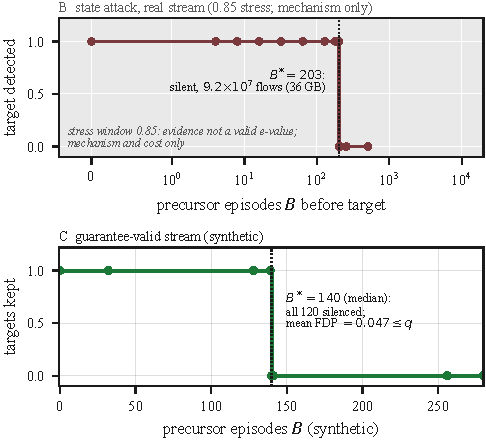
\includegraphics[width=\columnwidth]{figA_addis_state.pdf}
\caption{Manipulating ADDIS's spending state. \textbf{B}: on the real stress window, precursors silence
every rejection permanently at exactly the \cref{thm:addis} threshold --- on evidence that is not a
valid e-value, so this measures the mechanism and its cost, not an $\FDR$-valid outcome. \textbf{C}: the
same poisoning on synthetic streams where ADDIS's guarantee genuinely holds still silences every target.
Panel labels follow the earlier draft's combined figure so that the appendix tables read against it
unchanged.}
\label{fig:addis}
\end{figure}
\begin{table}[t]
\centering
\caption{ADDIS controller-state attack: $B^\ast=203$ precursor episodes
permanently silence the controller at position 0.85 --- the \textbf{known-invalid} stress window,
which is where the real-stream demonstration must sit, since ADDIS's horizon escape and its
guarantee-invalidity are the same property on two-point conformal evidence
(\cref{apptab:addissynth} reproduces the mechanism where the guarantee does hold). The break-even is
the number of detected episodes whose per-episode padding cost equals the whole one-off state
attack. All counts here use the \textbf{first-flow} within-bucket order, the optimistic upper bound over the orders we audit, not the canonical metadata-hash order \cref{tab:main} reports (\cref{apptab:ordering}); the order shifts detections and the level an alert fires at, and shifts nothing else.}
\label{apptab:addisstate}
\resizebox{\columnwidth}{!}{%
\begin{tabular}{ll}
\toprule
quantity & value \\
\midrule
$B^{\ast}$ (precursor episodes, $R=0$) & $203$ \\
per-precursor cost $\lfloor\lambda(\lvert C\rvert+1)/k\rfloor+1$ & $453{,}279$ flows \\
total attack flows & $92{,}015{,}637$ ($\approx 9.2\times10^{7}$) \\
level-saturated coincidence & $101$ of $147$ \\
minimal pad lands in window & $101$ of $147$ \\
median pad per episode (alternative) & $34{,}465{,}311$ flows \\
break-even vs padding & $2.67$ episodes \\
grey-box landing band ($\hat{\lvert C\rvert}/\lvert C\rvert$) & $[0.67,\,1.33]$ \\
\bottomrule
\end{tabular}}
\end{table}

\begin{table}[t]
\centering
\caption{The ADDIS state attack on a \textbf{synthetic stream where ADDIS's guarantee genuinely
holds}, isolating the mechanism from the real-window validity failure. The two-point conformal
evidence used elsewhere cannot supply this: its ADDIS horizon-escape (the spending index never
advances) is the \emph{same} property that makes its null p-values non-conservative, so no two-point
stream is both escape-feasible and guarantee-valid. We therefore use genuinely uniformly-conservative
null p-values ($\mathrm{Unif}(0,1)$, independent, the assumption ADDIS needs). The stream is
synthetic, so LSPR23's grouping plays no part and the result is \textbf{order-invariant} by
construction. \emph{Top:} ADDIS
controls $\FDR$ --- an expectation, not a per-realisation bound (the mixed arm's worst single
realisation is $\FDP=0.104$, above $q$, which the guarantee permits) --- on this
stream: the honest \emph{all-null} test (every rejection false) gives mean $\FDP=0.010\le q{=}0.05$, and with 120
strong targets present mean $\FDP=0.047$ at recall
1.00 (200 seeds each). \emph{Bottom:} the attack is adversarial state \emph{poisoning} ---
prepending $B$ attacker-generated \emph{alternative} (non-null) precursor episodes with
$p\in(\lambda,\tau]$. ADDIS constrains only \emph{true-null} p-values, so alternatives may take any
value: the legitimate nulls stay $\mathrm{Unif}(0,1)$ and ADDIS's guarantee holds on the \emph{attacked}
stream, not merely the clean one. These selected non-candidates advance the spending index and silence
every rejection at a median $B^{\star}=140$ over 300 guarantee-valid streams
(range 140--255; the tail from a rare null false positive that transiently
restores wealth). So even where ADDIS's guarantee holds \emph{after} the attack, an adversary who only
adds traffic drives the controller to silence --- a property of the mechanism, not an artefact of the
dataset already violating the assumption.}
\label{apptab:addissynth}
\begin{tabular}{lrr}
\toprule
 & mean $\FDP$ & $\le q{=}0.05$? \\
\midrule
all-null (every rejection false) & 0.010 & yes \\
mixed (120 targets, recall 1.00) & 0.047 & yes \\
\midrule
\multicolumn{3}{l}{\emph{state poisoning: median $B^{\star}{=}140$ (range 140--255) silences all}} \\
\bottomrule
\end{tabular}
\end{table}


%% ---------------------------------------------------------------------------------------
\section{Secondary Operational Baselines and Negative Results}\label{app:baselines}\label{app:negative}

\subsection{Matched operating points}

Comparing a $q=0.05$ procedure against an arbitrary classifier threshold measures nothing, so
\cref{apptab:frontier,apptab:frontier85} place every method on the achievable frontier of the
episode-max-score threshold family at its own budget, an ex-post oracle whose thresholds use the test
labels. Every method sits within $0.047$ recall of the best achievable point at its budget, so the
comparison that matters is choice of point: at the primary window e-LOND operates at 3 alerts, recall
$0.011$, $\FDP\,0.000$ under the canonical order (18 and $0.065$ under first-flow arrival), while an
ex-post oracle at the same zero error reaches recall $0.378$ on 104 alerts. Sweeping $q$ twenty-fold
moves median recall by $0.088$, while switching the spending sequence at fixed $q$ moves it by $0.188$
(first-flow paired sweep, \cref{apptab:qsweep}): formal error control can reduce the operator's freedom
over the workload--recall tradeoff.

\begin{table}[t]
\centering
\caption{Matched operating points at the \textbf{primary analysis window} (position 0.55, two-hour
grouping, $T = 57{,}368$ episodes of which 275 are malicious; every $\FDR$ statement conditional on
\cref{assump:groupval,lem:groupval}). Rows are under the \textbf{canonical} within-bucket order, as
\cref{tab:main} is, with the first-flow arm --- the optimistic upper bound --- beneath for the four rows
the order moves. The stress-test window 0.85 is \cref{apptab:frontier85}; the negative result, every
method within $0.047$ recall of the frontier, holds at both and under every order audited. The frontier
is an ex-post oracle (thresholds use the test labels) and is \emph{measured} order-invariant here, so it
is quoted once. The slot rule is an expectation over slots and the no-feedback threshold never updates,
so both are order-free by construction and verified unchanged.}
\label{apptab:frontier}
\resizebox{\columnwidth}{!}{%
\begin{tabular}{lrrrr}
\toprule
Method & alerts & $\FDP$ & recall & gap \\
\midrule
\multicolumn{5}{l}{\emph{canonical metadata-hash order}} \\
online FDR (mean rule)   & 3      & 0.000 & 0.011 & $+0.000$ \\
online FDR (slot rule)   & 91.0   & 0.000 & 0.331 & $+0.000$ \\
feedback, $L{=}0$        & 117    & 0.068 & 0.396 & $+0.000$ \\
feedback, $L{=}20$       & 137    & 0.204 & 0.396 & $+0.015$ \\
feedback, $L{=}50$       & 163    & 0.331 & 0.396 & $+0.044$ \\
fixed threshold          & 1{,}047 & 0.836 & 0.625 & $+0.000$ \\
\midrule
\multicolumn{5}{l}{\emph{first-flow arrival (optimistic upper bound; unmoved rows omitted)}} \\
online FDR (mean rule)   & 18     & 0.000 & 0.065 & $+0.000$ \\
feedback, $L{=}0$        & 119    & 0.076 & 0.400 & $-0.004$ \\
feedback, $L{=}20$       & 135    & 0.185 & 0.400 & $+0.004$ \\
feedback, $L{=}50$       & 150    & 0.267 & 0.400 & $+0.040$ \\
\midrule
\emph{frontier, $\FDP{=}0.000$} & 104 & 0.000 & \emph{0.378} & --- \\
\emph{frontier, $\FDP{=}0.050$} & 110 & 0.009 & \emph{0.396} & --- \\
\bottomrule
\end{tabular}}
\end{table}

\subsection{Analyst-feedback controllers}

The three feedback baselines of \cref{apptab:feedback} are threshold controllers, not $\FDR$ procedures.
Each carries a single state $u_t\in[0,1]$, a position in the calibration score distribution: it alerts on
episode $t$ when that episode's maximum flow score exceeds the $u_t$-quantile of the calibration scores,
and moves $u_t$ only when an analyst's disposition of an earlier alert arrives, after a wall-clock delay
$L$. Writing $\widehat{\FDP}_t$ for the false fraction over the last 200 dispositions received so far and
$\varepsilon_t=\widehat{\FDP}_t-q$,
{\small\begin{align*}
\textbf{P:}\ &u_{t+1}=u_t+\eta_P\,\varepsilon_t,\\
\textbf{PI:}\ &u_{t+1}=u_t+\eta_P\,\varepsilon_t+\eta_I\textstyle\sum_{r\le t}\varepsilon_r,\\
\textbf{AQT:}\ &u_{t+1}=u_t+\eta\big[(1{-}q)\mathbf 1\{\text{false}\}-q\mathbf 1\{\text{true}\}\big],
\end{align*}}%
with the PI integral clamped against windup and $u$ clipped to $[0,1]$. Gains are chosen per window,
delay and controller by grid search ($\eta_P\in\{0.005,0.02,0.05,0.2\}$, window $\in\{50,200\}$,
$u_0\in\{0.99,0.999\}$, AQT $\eta\in\{10^{-4},10^{-3},5\times10^{-3},0.02\}$, $\eta_I=\eta_P/10$)
minimising $(\lvert\FDP-q\rvert,-\text{recall})$ on the realised test labels, an ex-post oracle, so the
reported performance is an upper bound, the conservative direction for the negative conclusion. Under
first-flow order they reach $\FDP\,0.402$ (P, PI) and $0.523$ (AQT) at fifteen-minute disposition delay,
agree with one another by four hours, and reach the no-feedback threshold ($0.841$) only by eight: a
statement about delay on these controllers, not about feedback-aware testing~\cite{lu2026gaif}, whose
input our measurement prices.

\begin{table}[t]
\centering
\caption{Matched operating points at the \textbf{stress-test window} (position 0.85, two-hour
grouping, $T = 31{,}568$ episodes of which 255 are malicious).
$\FDP$ is measured against labels at a window where the evidence is \emph{not} a valid e-value
(\cref{sec:tail}). Rows are under the \textbf{canonical} within-bucket order, with the first-flow
arm beneath for the 4 rows the order moves; the frontier is measured
order-invariant and quoted once. The companion primary-window table is \cref{apptab:frontier}.}
\label{apptab:frontier85}
\resizebox{\columnwidth}{!}{%
\begin{tabular}{lrrrr}
\toprule
Method & alerts & $\FDP$ & recall & gap \\
\midrule
\multicolumn{5}{l}{\emph{canonical metadata-hash order}} \\
online FDR (mean rule) & 34 & 0.000 & 0.133 & $+0.000$ \\
online FDR (slot rule) & 126.6 & 0.001 & 0.496 & $-0.003$ \\
feedback, $L{=}0$ & 160 & 0.069 & 0.584 & $+0.004$ \\
feedback, $L{=}20$ & 171 & 0.117 & 0.592 & $+0.024$ \\
feedback, $L{=}50$ & 190 & 0.184 & 0.608 & $+0.047$ \\
fixed threshold & 875 & 0.763 & 0.812 & $+0.000$ \\
\midrule
\multicolumn{5}{l}{\emph{first-flow arrival (optimistic upper bound; unmoved rows omitted)}} \\
online FDR (mean rule) & 72 & 0.000 & 0.282 & $+0.000$ \\
feedback, $L{=}0$ & 161 & 0.068 & 0.588 & $+0.000$ \\
feedback, $L{=}20$ & 160 & 0.081 & 0.576 & $+0.012$ \\
feedback, $L{=}50$ & 171 & 0.140 & 0.576 & $+0.039$ \\
\midrule
\emph{frontier, $\FDP{=}0.000$} & 117 & 0.000 & \emph{0.459} & --- \\
\emph{frontier, $\FDP{=}0.050$} & 156 & 0.045 & \emph{0.584} & --- \\
\bottomrule
\end{tabular}}
\end{table}

\begin{table}[t]
\centering
\caption{Analyst-feedback controllers under wall-clock disposition delay ($q=0.05$) at the
\textbf{primary analysis window} (0.55); $\FDP$ is the two-seed mean. ``open-loop'' and ``at limit''
are for the P controller (open-loop is identical for PI). The final row is the long-span window at a
24\,h delay, where feedback collapses to the no-feedback open-loop baseline. All counts here use the \textbf{first-flow} within-bucket order, the optimistic upper bound over the orders we audit, not the canonical metadata-hash order \cref{tab:main} reports (\cref{apptab:ordering}); the order shifts detections and the level an alert fires at, and shifts nothing else.}
\label{apptab:feedback}
\resizebox{\columnwidth}{!}{%
\begin{tabular}{lrrrrr}
\toprule
delay (h) & $\FDP$ (P) & $\FDP$ (PI) & $\FDP$ (AQT) & \% open-loop & \% at limit \\
\midrule
0 & 0.053 & 0.049 & 0.172 & 0.9\% & 95.0\% \\
0.25 & 0.402 & 0.402 & 0.523 & 51.4\% & 87.3\% \\
1 & 0.514 & 0.514 & 0.592 & 60.5\% & 73.4\% \\
4 & 0.671 & 0.671 & 0.671 & 77.8\% & 44.7\% \\
8 & 0.834 & 0.834 & 0.834 & 99.8\% & 12.0\% \\
\midrule
long-span, 24\,h & 0.877 & 0.877 & 0.876 & \multicolumn{2}{c}{no-feedback $\FDP=0.887$} \\
\bottomrule
\end{tabular}}
\end{table}


\subsection{Negative results}

\emph{Inflation and fragmentation fail analytically.} For a purely benign group, conditioning on its
metadata $\sigma$-field gives $\mathbb E[\Ev(G)\mid\mathcal M_j]\le1<1/\alphat$, so no padding turns a
benign group into a discovery. For a pure-attack group whose flows fire independently with probability
$\phi$, $\mathbb E[\Ev(G)]=\phi\ceil$ is independent of the group size, so splitting a campaign across
groups does not lower per-group evidence. \emph{Boosting recovers nothing for two-point evidence:} the
optimal e-to-e boosting factor for a $\{0,\ceil\}$-valued e-value is $b^{\star}=1$ by construction.
\emph{Raising $k$} removes the operating point rather than trading power for validity; \emph{randomised
smoothing} removes the floor but not the reliably-detected set (\cref{app:taxonomy}); \emph{asymmetric
weighting} is not a free mitigation (\cref{sec:fixes}); \emph{stratified (Mondrian) conformal} does not
repair the position-0.85 anomaly; and the published $\alpha$-death fix (mem-e-LORD) is identical to e-LORD
before the first rejection.

\end{document}
